% ***************************************************************************************************
%
%	Szablon pracy magisterskiej dla Politechniki Wrocławskiej w wersji dwustronnej.
%	Autor:	Tomasz Strzałka
%   Korekta i dostosowanie do wymogów WIT 3.12.2021: dr inż. Anna Lauks-Dutka
%
% ***************************************************************************************************

% Styl dwustronny z domyślną wielkością czcionki 10pt oraz oddzieloną stroną tytułową (titlepage).
% Domyślnie rodziały rozpoczynają się na stronie prawej (openright).
\documentclass[10pt]{book}
\usepackage{times}


% ***************************************************************************************************
% Ustawienia języka
% ***************************************************************************************************

% Podstawowe ustawienia języka, według którego formatowany będzie dokument
\usepackage[polish]{babel}

% Pakiet babel dla polskiego języka powoduje konflikt z pakietem amssymb.
% Polecenie '\lll' definiują oba pakiety - porządana jest druga definicja.
\let\lll\undefined

% W przypadku wielojęzykowości ustawia główny język dokumentu
\selectlanguage{polish}

% Kodowanie dokumentu
\usepackage[utf8x]{inputenc}

% Dowolny rozmiar czcionek, kodowanie znaków
\usepackage{lmodern}

% Polskie wcięcia akapitów
\usepackage{indentfirst}

% Polskie łamanie wyrazów
\usepackage[plmath]{polski}

% Przecinek w wyrażeniach matematycznych zamiast kropki
\usepackage{icomma}

% Polskie formatowanie typograficzne
\frenchspacing

% Zapewnia liczne usprawnienia wyświetlania i organizacji matematycznych formuł. 
\usepackage{amsmath}

% Wprowadza rozszerzony zestaw symboli m.in. \leadsto
\usepackage{amssymb}

% Dodatkowa, ,,kręcona'' czcionka matematyczna
\usepackage{mathrsfs}

% Dodatkowe wsparcie dla środowiska mathbb, które nie wspiera domyślnie cyfr (\mathbb{})
\usepackage{bbold}

% Fixes/improves amsmath
\usepackage{mathtools}


% ***************************************************************************************************
% Kolory  
% ***************************************************************************************************

% Umożliwia kolorowanie poszczególnych komórek tabeli
\usepackage[table]{xcolor}% http://ctan.org/pkg/

% Umożliwia łatwą zmianę koloru linii w tabeli
\usepackage{tabu}

% Umożliwia rozszerzoną kontrolę nad kolorami.
\usepackage{xcolor}

% Definicje kolorów
\definecolor{lgray}{HTML}{9F9F9F}
\definecolor{dgray}{HTML}{5F5F5F}
% lgray				-	nazwa nowo zdefiniowanego koloru
% HTML				-	model kolorów
% CCCCCC			-	wartość koloru zgodna z modelem

% ***************************************************************************************************
% Algorytmy 
% ***************************************************************************************************

% Udostępnia środowisko do konstruowania pseudokodów
\usepackage[ruled,vlined,linesnumbered,longend,algochapter]{algorithm2e}
% ruled	- poziome kreski na początku i końcu algorytmu, podpis na górze oddzielony również kreską poziomą
% vlined - pionowe kreski łączące początek polecenia z jego końcem
% linesnumbered	- numerowanie kolejnych wierszy algorytmu
% longend - długie końcówki np. ifend, forend itd.
% algochapter - numeracja z rozdziałami

% Zamiana nazwy środowiska z domyślnej "Algorithm X" na "Pseudokod X"
\newenvironment{pseudokod}[1][htb]{
	\renewcommand{\algorithmcfname}{Pseudokod}
	\begin{algorithm}[#1]%
	}{
\end{algorithm}
}

% Zmiana rozmiaru komentarzy
\newcommand\algcomment[1]{
	\footnotesize{#1}
}

% Ustawienie zadanego stylu dla komentarzy
\SetCommentSty{algcomment}

% Wyśrodkowana tylda
\usepackage{textcomp}%
\newcommand{\textapprox}{\raisebox{0.5ex}{\texttildelow}}

% Listowanie kodów źródłowych
\usepackage{listings} 
\renewcommand{\lstlistingname}{Kod źródłowy} % Polska nazwa listingu

% Definicje pecjalnych znaków, które nie są obsługiwane w środowisku listing
\lstset{literate=
	{ż}{{\.{z}}}1	{ź}{{\'{z}}}1
	{ć}{{\'{c}}}1	{ń}{{\'{n}}}1
	{ą}{{\c a}}1	{ś}{{\'{s}}}1
	{ł}{{\l}}1		{ę}{{\c{e}}}1
	{ó}{{\'{o}}}1	{á}{{\'a}}1
	{é}{{\'e}}1		{í}{{\'i}}1
	{ó}{{\'o}}1		{ú}{{\'u}}1
	{ù}{{\`u}}1		{Á}{{\'A}}1
	{É}{{\'E}}1		{Í}{{\'I}}1
	{Ó}{{\'O}}1		{Ú}{{\'U}}1
	{à}{{\`a}}1		{è}{{\'e}}1
	{ì}{{\`i}}1		{ò}{{\`o}}1
	{ò}{{\`o}}1		{À}{{\`A}}1
	{È}{{\'E}}1		{Ì}{{\`I}}1
	{Ò}{{\`O}}1		{Ò}{{\`O}}1
	{ä}{{\"a}}1		{ë}{{\"e}}1
	{ï}{{\"i}}1		{ö}{{\"o}}1
	{ü}{{\"u}}1		{Ä}{{\"A}}1
	{Ë}{{\"E}}1		{Ï}{{\"I}}1
	{Ö}{{\"O}}1		{Ü}{{\"U}}1
	{â}{{\^a}}1		{ê}{{\^e}}1
	{î}{{\^i}}1		{ô}{{\^o}}1
	{û}{{\^u}}1		{Â}{{\^A}}1
	{Ê}{{\^E}}1		{Î}{{\^I}}1
	{Ô}{{\^O}}1		{Û}{{\^U}}1
	{œ}{{\oe}}1		{Œ}{{\OE}}1
	{æ}{{\ae}}1		{Æ}{{\AE}}1
	{ß}{{\ss}}1		{ç}{{\c c}}1
	{Ç}{{\c C}}1	{ø}{{\o}}1
	{å}{{\r a}}1	{Å}{{\r A}}1
	{€}{{\EUR}}1	{£}{{\pounds}}1
}

% ***************************************************************************************************
% Marginesy 
% ***************************************************************************************************

% Ustawienia rozmiarów stron i ich marginesów
%korekta ALD - dodatkowe 0.5cm na oprawę z lewej
%\usepackage[headheight=18pt, top=25mm, bottom=25mm, left=25mm, right=25mm]{geometry}
\usepackage[headheight=18pt, top=25mm, bottom=25mm, left=30mm, right=25mm]{geometry}
% headheight		-	wysokość tytułów
% top				-	margines górny
% bottom			-	margines dolny
% left				-	margines lewy
% right				-	margines prawy

% Usunięcie górnego marginesu dla środowisk
\makeatletter
\setlength\@fptop{0\p@}	
\makeatother

% ***************************************************************************************************
% Styl 
% ***************************************************************************************************

% Definiuje środowisko 'titlingpage', które zapewnia pełną kontrolę nad układem strony tytułowej.
\usepackage{titling}


% Umożliwia modyfikowanie stylu spisu treści
\usepackage{tocloft}	

\tocloftpagestyle{tableOfContentStyle}

% Definiowanie własnych stylów nagłówków i/lub stopek
\usepackage{fancyhdr}

% Domyślny styl dla pracy 
\fancypagestyle{custom}{
	\fancyhf{}									% wyczyść stopki i nagłówki
	\fancyhead[RO]{								% Prawy, nieparzysty nagłówek
%korekta ALD: 
%\hrulefill \hspace{16pt} \large Rozdział \thechapter
		\hrulefill \hspace{16pt} \large \ifnum \thechapter>0 {Rozdział \thechapter} \else{Wstęp}\fi
		\put(-472.1, 12.1){%
			\makebox(0,0)[l]{%
                
\includegraphics[width=0.05\textwidth]{figures/pwr-logo}
			}
		}
		\put(-443,5.5){%
			\makebox(0,0)[l]{%
				\small Politechnika Wrocławska
			}
		}
	}
	\fancyhead[LE]{								% Lewy, parzysty nagłówek
%korekta ALD: 
%\large Rozdział \thechapter \hspace{16pt} \hrulefill 
        \large \ifnum \thechapter>0 {Rozdział \thechapter} \else{Wstęp}\fi \hspace{16pt} \hrulefill 
		\put(-22, 12.1){%
			\makebox(0,0)[l]{%
                %korekta ALD
				%
\includegraphics[width=0.05\textwidth]{figures/pwr-logo}
                
\includegraphics[width=0.05\textwidth]{figures/wit-logo}			}
		}
		\put(-210,5.5){%
			\makebox(0,0)[l]{%
%				\small Wydział Podstawowych Problemów Techniki
%Korekta ALD
\small Wydział Informatyki i Telekomunikacji
			}
		}
	}
	\fancyfoot[LE,RO]{							% Stopki
		\thepage
	}
	\renewcommand{\headrulewidth}{0pt}			% Grubość linii w nagłówku
	\renewcommand{\footrulewidth}{0.2pt}		% Grubość linii w stopce
}


% Domyślny styl dla bibliografii
\fancypagestyle{bibliographyStyle}{
	\fancyhf{}									% wyczyść stopki i nagłówki
	\fancyhead[RO]{								% Prawy, nieparzysty nagłówek
		\hrulefill \hspace{16pt} \large Dodatek \thechapter
		\put(-472.1, 12.1){%
			\makebox(0,0)[l]{%
	
\includegraphics[width=0.05\textwidth]{figures/pwr-logo}
			}
		}
		\put(-443,5.5){%
			\makebox(0,0)[l]{%
				\small Politechnika Wrocławska
			}
		}
	}
	\fancyhead[LE]{								% Lewy, parzysty nagłówek
		\large Bibliografia \hspace{16pt} \hrulefill 
		\put(-22, 12.1){%
			\makebox(0,0)[l]{%
			%korekta ALD	\includegraphics[width=0.05\textwidth]{wppt-logo}
			
\includegraphics[width=0.05\textwidth]{figures/wit-logo}
			}
		}
		\put(-210,5.5){%
			\makebox(0,0)[l]{%
			%korekta ALD
				%\small Wydział Podstawowych Problemów Techniki
				\small Wydział Informatyki i Telekomunikacji
			}
		}
	}
	\fancyfoot[LE,RO]{							% Stopki
		\thepage
	}
	\renewcommand{\headrulewidth}{0pt}			% Grubość linii w nagłówku
	\renewcommand{\footrulewidth}{0.2pt}		% Grubość linii w stopce
}

% Domyślny styl dla spisu tabel i rysunków
\fancypagestyle{listOfTablesStyle}{
	\fancyhf{}									% wyczyść stopki i nagłówki
	\fancyhead[RO]{								% Prawy, nieparzysty nagłówek
		\hrulefill \hspace{16pt} \large Spis tabel
		\put(-472.1, 12.1){%
			\makebox(0,0)[l]{%
			
\includegraphics[width=0.05\textwidth]{figures/pwr-logo}
			}
		}
		\put(-443,5.5){%
			\makebox(0,0)[l]{%
				\small Politechnika Wrocławska
			}
		}
	}
	\fancyhead[LE]{								% Lewy, parzysty nagłówek
		\large Spis tabel \hspace{16pt} \hrulefill 
		\put(-22, 12.1){%
			\makebox(0,0)[l]{%

\includegraphics[width=0.05\textwidth]{figures/wit-logo}
			}
		}
		\put(-210,5.5){%
			\makebox(0,0)[l]{%
				\small Wydział Informatyki i Telekomunikacji
			}
		}
	}
	\fancyfoot[LE,RO]{							% Stopki
		\thepage
	}
	\renewcommand{\headrulewidth}{0pt}			% Grubość linii w nagłówku
	\renewcommand{\footrulewidth}{0.2pt}		% Grubość linii w stopce
}

\fancypagestyle{listOfPlotsStyle}{
	\fancyhf{}									% wyczyść stopki i nagłówki
	\fancyhead[RO]{								% Prawy, nieparzysty nagłówek
		\hrulefill \hspace{16pt} \large Spis rysunków
		\put(-472.1, 12.1){%
			\makebox(0,0)[l]{%
			
\includegraphics[width=0.05\textwidth]{figures/pwr-logo}
			}
		}
		\put(-443,5.5){%
			\makebox(0,0)[l]{%
				\small Politechnika Wrocławska
			}
		}
	}
	\fancyhead[LE]{								% Lewy, parzysty nagłówek
		\large Spis rysunków \hspace{16pt} \hrulefill 
		\put(-22, 12.1){%
			\makebox(0,0)[l]{%

\includegraphics[width=0.05\textwidth]{figures/wit-logo}
			}
		}
		\put(-210,5.5){%
			\makebox(0,0)[l]{%
				\small Wydział Informatyki i Telekomunikacji
			}
		}
	}
	\fancyfoot[LE,RO]{							% Stopki
		\thepage
	}
	\renewcommand{\headrulewidth}{0pt}			% Grubość linii w nagłówku
	\renewcommand{\footrulewidth}{0.2pt}		% Grubość linii w stopce
}

% Domyślny styl dla dodatków
\fancypagestyle{appendixStyle}{
	\fancyhf{}									% wyczyść stopki i nagłówki
	\fancyhead[RO]{								% Prawy, nieparzysty nagłówek
		\hrulefill \hspace{16pt} \large Załącznik \thechapter
		\put(-472.1, 12.1){%
			\makebox(0,0)[l]{%

\includegraphics[width=0.05\textwidth]{figures/pwr-logo}
			}
		}
		\put(-443,5.5){%
			\makebox(0,0)[l]{%
				\small Politechnika Wrocławska
			}
		}
	}
	\fancyhead[LE]{								% Lewy, parzysty nagłówek
		\large Załącznik \thechapter \hspace{16pt} \hrulefill 
		\put(-22, 12.1){%
			\makebox(0,0)[l]{%
%korekta ALD:				\includegraphics[width=0.05\textwidth]{wppt-logo}

\includegraphics[width=0.05\textwidth]{figures/wit-logo}
			}
		}
		\put(-210,5.5){%
			\makebox(0,0)[l]{%
			%korekta ALD
				%\small Wydział Podstawowych Problemów Techniki
				\small Wydział Informatyki i Telekomunikacji
			}
		}
	}
	\fancyfoot[LE,RO]{							% Stopki
		\thepage
	}
	\renewcommand{\headrulewidth}{0pt}			% Grubość linii w nagłówku
	\renewcommand{\footrulewidth}{0.2pt}		% Grubość linii w stopce
}

% Osobny styl dla stron zaczynających rozdział/spis treści itd. (domyślnie formatowane jako "plain")
\fancypagestyle{chapterBeginStyle}{
	\fancyhf{}%
	\fancyfoot[LE,RO]{
		\thepage
	}
	\renewcommand{\headrulewidth}{0pt}
	\renewcommand{\footrulewidth}{0.2pt}
}

% Styl dla pozostałych stron spisu treści
\fancypagestyle{tableOfContentStyle}{
	\fancyhf{}%
	\fancyfoot[LE,RO]{
		\thepage
	}
	\renewcommand{\headrulewidth}{0pt}
	\renewcommand{\footrulewidth}{0.2pt}
}
% Formatowanie tytułów rozdziałów i/lub sekcji
\usepackage{titlesec}

% Formatowanie tytułów rozdziałów
\titleformat{\chapter}[hang]					% kształt
{
	\vspace{-10ex}
	%\Huge
	\large
	\bfseries
}												% formatowanie tekstu modyfikowanego elementu
{}												% etykieta występująca przed tekstem modyfikowanego elementu, niewidoczna w spisie treści
{
	10pt
}												% odstęp formatowanego tytułu od lewego marginesu/etykiety
{
    \large
	\bfseries
}												% formatowanie elementów przed modyfikowanym tytułem
[
\vspace{2ex}
%\rule{\textwidth}{0.4pt}
%\vspace{-4ex}
]												% dodatkowe formatowanie stosowane poniżej modyfikowanego tytułu


% Formatowanie tytułów sekcji
\titleformat{\subsection}[hang]					% kształt
{
	\vspace{2ex}
%	\titlerule\vspace{1ex}
	\large\bfseries
}												% formatowanie tekstu modyfikowanego elementu
{
	\thesection									% etykieta występująca przed tekstem modyfikowanego elementu, niewidoczna w spisie treści
}
{
	0pt
}												% odstęp formatowanego tytułu od lewego marginesu/etykiety
{
	\large
	\bfseries
}												% formatowanie elementów przed modyfikowanym tytułem


%ALD- ustawienia wielkości fontów dla rozdziałów i sekcji
\usepackage{sectsty}
%\chapterfont{\fontsize{14}{17.6}\selectfont}
\subsectionfont{\fontsize{13}{16.8}\selectfont}
\subsectionfont{\fontsize{12}{15.6}\selectfont}

% ***************************************************************************************************
% Linki
% ***************************************************************************************************

% Umożliwia wstawianie hiperłączy do dokumentu
\usepackage{hyperref}							% Aktywuje linki

\hypersetup{
	colorlinks	=	true,					% Koloruje tekst zamiast tworzyć ramki.
	linkcolor		=	blue,					% Kolory: referencji,
        citecolor		=	blue,					% cytowań,
	urlcolor		=	blue					% hiperlinków.
}

% Do stworzenia hiperłączy zostanie użyta ta sama (same) czcionka co dla reszty dokumentu
\urlstyle{same}




% ***************************************************************************************************
% Linki
% ***************************************************************************************************

% Umożliwia zdefiniowanie własnego stylu wyliczeniowego
\usepackage{enumitem}

% Nowa lista numerowana z trzema poziomami
\newlist{myitemize}{itemize}{3}

% Definicja wyglądu znacznika pierwszego poziomu
\setlist[myitemize,1]{
	label		=	\textbullet,
	leftmargin	=	4mm}

% Definicja wyglądu znacznika drugiego poziomu
\setlist[myitemize,2]{
	label		=	$\diamond$,
	leftmargin	=	8mm}

% Definicja wyglądu znacznika trzeciego poziomu
\setlist[myitemize,3]{
	label		=	$\diamond$,
	leftmargin	=	12mm
}

% ***************************************************************************************************
% Inne pakiety
% ***************************************************************************************************

% Dołączanie rysunków
\usepackage{graphicx}

% Figury i przypisy
\usepackage{caption}
\usepackage{subcaption}

% Umożliwia tworzenie przypisów wewnątrz środowisk
\usepackage{footnote}

% Umożliwia tworzenie struktur katalogów
\usepackage{dirtree}

% Rozciąganie komórek tabeli na wiele wierszy
\usepackage{multirow}

% Precyzyjne obliczenia szerokości/wysokości dowolnego fragmentu wygenerowanego przez LaTeX
\usepackage{calc}

\usepackage{float} 

% ***************************************************************************************************
% Matematyczne skróty
% ***************************************************************************************************

% Skrócony symbol liczb rzeczywistych
\newcommand{\RR}{\mathbb{R}}

% Skrócony symbol liczb naturalnych
\newcommand{\NN}{\mathbb{N}}

% Skrócony symbol liczb wymiernych
\newcommand{\QQ}{\mathbb{Q}}

% Skrócony symbol liczb całkowitych
\newcommand{\ZZ}{\mathbb{Z}}

% Skrócony symbol logicznej implikacji
\newcommand{\IMP}{\rightarrow}

% Skrócony symbol  logicznej równoważności
\newcommand{\IFF}{\leftrightarrow}

% ***************************************************************************************************
% Środowiska
% ***************************************************************************************************

% Środowisko do twierdzeń
\newtheorem{theorem}{Twierdzenie}[chapter]

% Środowisko do lematów
\newtheorem{lemma}{Lemat}[chapter]

% Środowisko do przykładów
\newtheorem{example}{Przykład}[chapter]

% Środowisko do wniosków
\newtheorem{corollary}{Wniosek}[chapter]

% Środowisko do definicji
\newtheorem{definition}{Definicja}[chapter]

% Środowisko do dowodów
\newenvironment{proof}{
	\par\noindent \textbf{Dowód.}
}{
\begin{flushright}
	\vspace*{-6mm}\mbox{$\blacklozenge$}
\end{flushright}
}

%ALD - nowe środowisko do streszczenia i abstractu
\newenvironment{streszczenie}{
	\par\noindent {\large \textbf{Streszczenie}\\[14pt]\indent}
}{}
\newenvironment{abstract}{
	\par\noindent {\large \textbf{Abstract}\\[14pt]\indent}
}{}

% Środowisko do uwag
\newenvironment{remark}{
	\bigskip \par\noindent \small \textbf{Uwaga.}
}{
\begin{small}
	\vspace*{4mm}
\end{small}
}

% ***************************************************************************************************
% Słownik
% ***************************************************************************************************

% Prawidłowe dzielenie wyrazów
% \hyphenation{wszy-stkich ko-lu-mnę każ-da od-leg-łość
% 	dzie-dzi-ny dzie-dzi-na rów-nych rów-ny
% 	pole-ga zmie-nna pa-ra-met-rów wzo-rem po-cho-dzi
% 	o-trzy-ma wte-dy wa-run-ko-wych lo-gicz-nie
% 	skreś-la-na skreś-la-ną cał-ko-wi-tych wzo-rów po-rzą-dek po-rząd-kiem
% 	przy-kład pod-zbio-rów po-mię-dzy re-pre-zen-to-wa-ne
% 	rów-no-waż-ne bi-blio-te-kach wy-pro-wa-dza ma-te-ria-łów
% 	prze-ka-za-nym skoń-czo-nym moż-esz na-tu-ral-na cią-gu tab-li-cy
% 	prze-ka-za-nej od-po-wied-nio}

% ***************************************************************************************************
% Dokument
% ***************************************************************************************************

\frontmatter

\begin{document}

    \pagestyle{empty}
	\begin{titlingpage}
		\vspace*{\fill}
		\begin{center}
			\begin{picture}(430,500)
				\put(60,590){\makebox(0,0)[l]{\huge \textbf{Politechnika Wrocławska}}}
				\put(40,565){\makebox(0,0)[l]{\Large \textbf{Wydział Informatyki i Telekomunikacji}}}
                \put(0,550){\line(1,0){430}}
                \put(0,510){\makebox(0,0)[l]{\large Kierunek: \textbf{INF-PPT}}}
                %\textbf{3 literowy kod kierunku}}}
                \put(0,490){\makebox(0,0)[l]{\large Specjalność: \textbf{-}}}                
                %\textbf{3 literowy kod specjalności}}}                
				\put(0,370){\begin{minipage}{0.9\textwidth}
				\centering
				\Huge \textsc{Praca Dyplomowa\\ Inżynierska}
                \end{minipage}
				}
% Tytuł pracy
				\put(0,230){\begin{minipage}{0.9\textwidth}
				\centering
				\LARGE \textbf{Bot do komputerowej gry wyścigowej}
                \end{minipage}
				}
% Autor pracy
				\put(0,170){\begin{minipage}{0.9\textwidth}
				\centering
				\Large {
				Kamil Matejuk
				}
				\end{minipage}
				}
% dane promotora
				\put(0,90){\begin{minipage}{0.9\textwidth}
				\centering
				\large{
				Opiekun pracy\\
				\textbf{Dr Marcin Michalski}
				}
				\end{minipage}
				}
				\put(0,-30){
				\begin{minipage}{0.9\textwidth}
				\normalsize{
				Słowa kluczowe: Bot, Uczenie maszynowe, Uczenie przez wzmacnianie
				}
				\end{minipage}
				}
                \put(0,-80){\line(1,0){430}}
				\put(155,-100){\makebox(0,0)[bl]{\large \textsc{Wrocław 2022}}}
			\end{picture}
		\end{center}	
		\vspace*{\fill}
	\end{titlingpage}
	
    \clearpage % \cleardoublepage
	\begin{streszczenie}
Tutaj tekst streszczenia po polsku. 
\end{streszczenie}

    \clearpage % \cleardoublepage
	\pagenumbering{Roman}
	\pagestyle{tableOfContentStyle}
	\tableofcontents

	% spis rysunków (opcjonalnie)    
	% \clearpage
	\pagestyle{listOfPlotsStyle}
	\listoffigures
	% \addcontentsline{toc}{chapter}{Spis rysunków}
	
	% spis tabel (opcjonalnie)
	% \clearpage
	% \renewcommand{\listtablename}{Spis tabel}
	\pagestyle{listOfTablesStyle}
	\listoftables
	% \addcontentsline{toc}{chapter}{Spis tabel}

    \clearpage % \cleardoublepage
    
		
	% ***************************************************************************************************
	% Wstęp
	% ***************************************************************************************************
	
	\pagestyle{custom}
	\mainmatter
	
	% ***************************************************************************************************
	% Rodziały
	% ***************************************************************************************************

	%Korekta ALD - nienumerowany wstęp
%\chapter{Wstęp}
\addcontentsline{toc}{chapter}{Wstęp}
\chapter*{Wstęp}

\thispagestyle{chapterBeginStyle}

Praca dyplomowa inżynierska jest dokumentem opisującym zrealizowany system techniczny. Praca powinna być napisana poprawnym językiem odzwierciedlającym aspekty techniczne (informatyczne) omawianego zagadnienia. Praca powinna być napisana w trybie bezosobowym (w szczególności należy unikać trybu pierwszej osoby liczby pojedynczej i mnogiej). Zdania opisujące konstrukcję systemu informatycznego powinny być tworzone w stronie biernej. W poniższym dokumencie przykłady sformułowań oznaczono kolorem niebieskim. W opisie elementów systemu, komponentów, elementów kodów źródłowych, nazw plików, wejść i wyjść konsoli należy stosować czcionkę stałej szerokości, np: {\color{lgray}zmienna \verb|wynik| przyjmuje wartość zwracaną przez funkcję \verb|dodaj(a,b)|, dla argumentów \verb|a| oraz \verb|b| przekazywanych \ldots}.

Układ poniższego dokumentu przedstawia wymaganą strukturę pracy, z rozdziałami zawierającymi analizę zagadnienia, opis projektu systemu oraz implementację (dobór podrozdziałów jest przykładowy i należy go dostosować do własnej tematyki pracy). 
  
Wstęp pracy (nie numerowany) powinien składać się z czterech części (które nie są wydzielane jako osobne podrozdziały): zakresu pracy, celu, analizy i porównania istniejących rozwiązań oraz przeglądu literatury, oraz opisu zawartości pracy.

Każdy rozdział powinien rozpoczynać się od akapitu wprowadzającego, w którym zostaje w skrócie omówiona zawartość tego rozdziału.

{\color{dgray}
Praca swoim zakresem obejmuje wielowarstwowe rozproszone systemy informatyczne typu ,,B2B'' wspierające wymianę danych pomiędzy przedsiębiorstwami. Systemy tego typu, konstruowane dla dużych korporacji, charakteryzują się złożoną strukturą poziomą i pionową, w której dokumenty \ldots

Celem pracy jest zaprojektowanie i oprogramowanie aplikacji o następujących założeniach funkcjonalnych:
\begin{itemize}
    \item wspieranie zarządzania obiegiem dokumentów wewnątrz korporacji z uwzględnieniem \ldots,
	\item wspieranie zarządzania zasobami ludzkimi z uwzględnieniem modułów kadrowych oraz \ldots,
	\item gotowość do uzyskania certyfikatu ISO \ldots,
	\item \ldots.
\end{itemize}

Istnieje szereg aplikacji o zbliżonej funkcjonalności: \ldots, przy czym \ldots.

Praca składa się z czterech rozdziałów.
W rozdziale pierwszym omówiono strukturę przedsiębiorstwa \ldots, scharakteryzowano grupy użytkowników oraz przedstawiono procedury związane z obiegiem dokumentów. Szczegółowo opisano mechanizmy \ldots. Przedstawiono uwarunkowania prawne udostępniania informacji \ldots, w ramach \ldots.

W rozdziale drugim przedstawiono szczegółowy projekt systemy w notacji UML. Wykorzystano diagramy \ldots.
Opisano w pseudokodzie i omówiono algorytmy generowania \ldots.

W rozdziale trzecim opisano technologie implementacji projektu: wybrany język programowania, biblioteki, system zarządzania bazą danych, itp.  Przedstawiono dokumentację techniczną kodów źródłowych interfejsów poszczególnych modułów systemu. Przedstawiono sygnatury metod publicznych oraz \ldots.

W rozdziale czwartym przedstawiono sposób instalacji i wdrożenia systemu w środowisku docelowym.

Końcowy rozdział stanowi podsumowanie uzyskanych wyników.
}


	\clearpage % \cleardoublepage

	\chapter{Stworzenie gry}
\thispagestyle{chapterBeginStyle}
\label{rozdzial1}

\SetKwComment{Comment}{/* }{ */}

\section{Cel i funkcjonalności}
Gra została stworzona przede wszystkim jako środowisko treningowe oraz testowe bota, dopiero w drugiej kolejności jako rozrywka dla użytkownika. Dostarczona w dodatku $A$ gra pozwala graczowi na załadowanie jednego z domyślnych terenów, bądź stworzenie własnego terenu i przetestowanie go w grze. Celem rozgrywki jest przetransportowanie pojazdu od miejsca startowego do mety, nie zjeżdżając ze ścieżki. Gra kończy się po wykonaniu jednego pełnego okrążenia. Gracz konkuruje z 3 innymi pojazdami, sterowanymi przez wytrenowanego bota. Dodatkowo gracz posiada możliwość stworzenia własnego terenu i trasy, sterując kilkoma parametrami. W ten sam sposób zostały przygotowane tereny, na których został wytrenowany bot.

\section{Wykorzystane technologie}
Gra została stworzona z wykorzystaniem silnika do gier Unity Engine 3D. Jest to jeden z dwóch najpopularniejszych silników do tworzenia gier, poza Unreal Engine, natomiast posiada on niższą barierę wejścia. Wykorzystanie Unity pozwoliło na zasymulowanie praw fizyki występujących przy prowadzeniu pojazdu.

\section{Stworzenie trasy 2D}
Pierwszym etapem generowania terenu jest wybór krzywej opisującej trasę. Każda wygenerowana trasa jest krzywą zamkniętą. Składa się ona z segmentów, których ilość jest bezpośrednio powiązana z zawiłością trasy. 

Aby wybrać końce segmentów, losowane są punkty $P=(P_x,P_y)$ na płaszczyźnie z uniwersalnym prawdopodobieństwem, z zakresu $P_x \in [-1, 1]$, $P_y \in [-1, 1]$, upewniając się że żadne 2 punkty nie są za blisko siebie.
\\\phantom{.}\\
\begin{algorithm}[H]
\caption{Wybór punktów trasy}\label{alg:two}
\KwData{\\
    $n \gets$ \textit{ilość segmentów}\;
    $d \gets$ \textit{minimalna odległość między punktami}\;}
$positions \gets []$\;
\While{$positions.Length < n$}{
    $pNew \gets$ \textit{new point}\;
    $pNew.x \gets random(-1, 1)$\;
    $pNew.y \gets random(-1, 1)$\;
    $tooClose \gets false$\;
    \ForEach{$P \in positions$}{
        \If{$distance(P, pNew) < d$}{
            $tooClose \gets true$\;
            $break$\;
        }
    }
    \If{\textit{not tooClose}}{
        \textit{add pNew. to positions}\;
    }
}
\end{algorithm}
\phantom{.}\\
Po wyborze odpowiedniej ilości punktów, sortowane są one zgodnie z ruchem wskazówek zegara, na podstawie kąta pomiędzy wektorem $[0, 1]$, a wektorem kończącym się w danym punkcie.
\\\\
\begin{algorithm}[H]
    \caption{Wyznaczenie kąta pomiędzy punktem a prostą OY}\label{alg:two}
    \KwData{$P \gets$ \textit{punkt}}
    $forwardVector \gets [0, 1].normalized$\;
    $pointVector \gets [P.x, P.y].normalized$\;
    $angle \gets acos(dot(forwardVector, pointVector))$ \Comment*[r]{Arcus cosinus iloczynu skalarnego}
    $sign \gets cross(forwardVector, pointVector).z$ \Comment*[r]{iloczyn wektorowy}
    \eIf{$sign \geq 0$}{
        \Return{$angle$}\;
        } {
        \Return{$-1 \cdot angle$}\;
    }
\end{algorithm}
\phantom{.}\\
Następnie trasa w każdym segmencie wyznaczana jest za pomocą krzywej Bezier 3 stopnia, ponieważ pozwala ona w stosunkowo prosty sposób zapisać stosunkowo komplikowane krzywe, utrzymując płynny kształt. Każda krzywa Bezier składa się z punktu startowego $P_0$, końcowego $P_3$, oraz dwóch punktów kontrolnych $P_1$, $P_2$, oraz wyraża sie wzorem:
\[ b(t) = (1 - t)^3 * P_0 + 3t(1-t)^2 * P_1 + 3t^2 (1-t) * P_2 + t^3 * P_3 \hspace{1cm}\textit{dla } t \in [0, 1] \]
Aby zapewnić płynne połączenia pomiędzy segmentami, sąsiednie punkty kontrolne powinny znajdować sie na tej samej prostej. Dla każdego punktu startowego wyznaczane są punkty kontrolne segmentu poprzednioego i następnego, na podstawie sąsiadujących punktów startowych.

Poniższy rysunek przedstawia trzy wylosowane punkty $A,B,C$, oraz proces generacji punktów kontrolnych dla środkowego punktu $B$. Na początku wyznaczana jest prosta prostopadła do dwusiecznej kąta pomiędzy wektorami $BA$ i $BC$, poprzez normalizację ww. wektorów odpowiednio do $BA'$ i $BC'$, a następnie odjęcie powstałych wektorów. Punkt kontrolny $D$ znajduje się na ww. prostej, w odległości równej połowie długości wektora $BA$. Analogicznie położony jest punkt kontrolny $E$. Po wykonaniu powyższych operacji dla każdego punktu startowego na wyznaczonej trasie, w każdym segmencie znajdują się oba punkty kontrolne. Po podstawieniu punktów startowych i kontrolnych (np. $A,F,D,B$) dla każdego segmentu wyznaczona zostanie cała trasa.

\begin{figure}[h]
    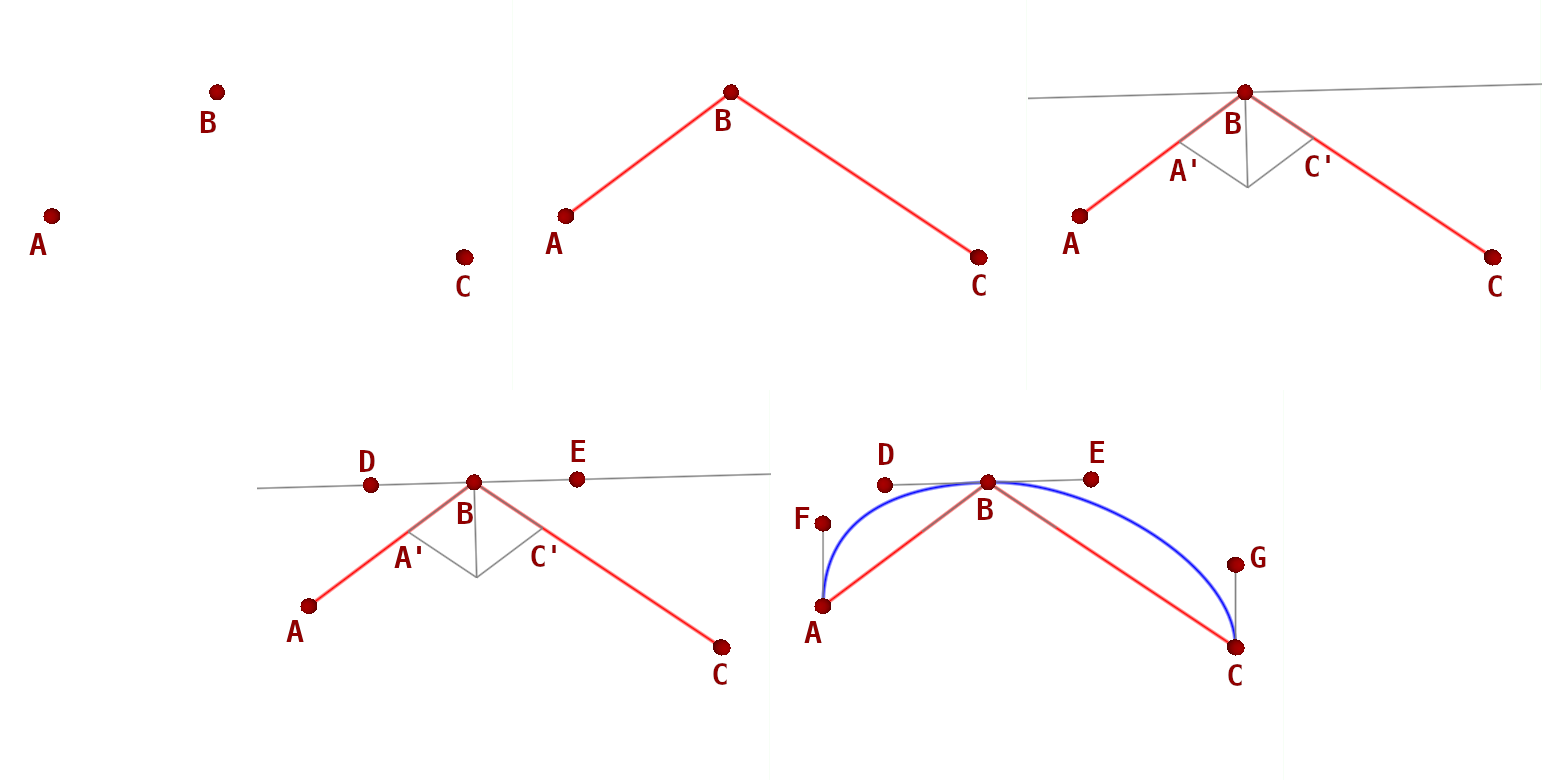
\includegraphics[width=\textwidth]{figures/loop_creation}
    \caption{Generowanie punktów kontrolnych krzywej Bezier}
    \label{fig}
\end{figure}

\section{Stworzenie terenu 3D}
Każdy stworzony teren gry jest rozmiaru $512 x 512$, z czego $10\%$ przeznaczone jest na marginesy z każdej strony, co pozostawia wewnętrzną przestrzeń $409 x 409$ na wygenerowany tor. Każdy punkt wygenerowanej pętli jest skalowany odpowiednio, aby trasa wypełniła całość dostępnej przestrzeni. Następnie dla każdego punktu terenu generowana jest wysokość, zdefiniowana jako procent maksymalnej wysokości $128$. Wysokość składa się z trzech warstw, wykorzystujących Szum Perlina, każda coraz bardziej szczegółowa. Implementacja Szumu Perlina została dostarczona jako fragment biblioteki $Mathf$ przez Unity \cite{PerlinNoise}.
\\\\
\begin{algorithm}[H]
    \caption{Wyznaczenie wysokości terenu}\label{alg}
    \KwData{\\
        $x \gets$ \textit{wspołrzędna X punktu}\;
        $y \gets$ \textit{wspołrzędna Y punktu}\;}
    $x \gets x + offsetX$\;
    $y \gets y + offsetY$\;
    $h1 \gets detailsMain \cdot PerlinNoise(x \cdot scaleMain, y \cdot scaleMain)$\;
    $h2 \gets detailsMinor \cdot PerlinNoise(x \cdot scaleMinor, y \cdot scaleMinor)$\;
    $h3 \gets detailsTiny \cdot PerlinNoise(x \cdot scaleTiny, y \cdot scaleTiny)$\;
    \Return{h1 + h2 + h3}
\end{algorithm}
\phantom{.}\\
Powyższa funkcja pozwala na sterowanie krztałtem terenu poprzez parametry $details$ i $scale$ dla każdej z trzech warstw $main$, $minor$, $tiny$. Warstwa $main$ definiuje ogólny krztałt terenu, warstwa $minor$ dodaje mniejsze pagórki, natomiast warstwa $tiny$ dodaje drobne detale. Dodatkowo poprzez sterowanie $offsetX$ i $offsetY$ możliwe jest przesunięcie wszystkich wartości w płaszczyźnie poziomej.

\section{Przypisanie tekstur}
Zależnie od rodzaju terenu, wybierany jest odpowiedni zestaw tekstur. Dla każdego punktu wygenerowanego terenu przypisane są odpowiednie wartości przezroczystości tekstur, tworząc jak najbardziej realistyczne krajobrazy. Decyzja o wybraniu przezroczystości tekstur została podjęta na podstawie rodzaju terenu wybranego przez użytkownika, wysokości danego punktu, kierunku płaszczyzny zbocza, kąta nachylenia zbocza oraz odległości punktu od centrum wygenerowanej trasy. Odczytanie wartości takich jak wysokość, kierunek płaszczyzny i kąt nachylenia można wykonać w stałym czasie $O(1)$. Natomiast znalezienie najbliższego punktu trasu jest bardziej złożonym procesem. Poniżej przedstawiono proces wyboru metody jego wyznaczania.

\subsection{Znalezienie najbliższego punktu krzywej Bezier}
Poniższa metoda dzieli każdy segment trasy na $m$ odcinków, a następnie iteruje wszystkie końce odcinków we wszystkich segmentach. Optymalna ilość podziału wyznaczona została eksperymentalnie. Metoda ta ma złożoność czasową $O(nm)$, gdzie $n$ oznacza liczbę segmentów trasy, natomiast $m$ oznacza dokładność podziałów danego segmentu.
\\\\
\begin{algorithm}[H]
    \caption{Znalezienie najbliższego punktu krzywej Bezier}\label{alg}
    \KwData{$P \gets$ \textit{cel poza krzywą}}
    $minDist \gets infinity$\;
    $minT \gets 0$\;
    \For{i = 0; i < 100; i++}{
        $t \gets i \cdot 0.01$\;
        $pProjection \gets B(t)$ \Comment*[r]{punkt w t\% długości krzywej bezier}
        $dist \gets distance(P, pProjection)$\;
        \If{dist < minDist}{
            $minDist \gets dist$\;
            $minT \gets t$\;
        }
    }
    \Return{B(minT)}
\end{algorithm}
\phantom{.}\\

\subsection{Udoskonalone znalezienie najbliższego punktu krzywej Bezier}
Poniższa metoda wywodzi się z artykułu \cite{ImprovedPointProjectionBezier}, oraz została przystosowana dla krzywej Bezier 3 stopnia.\\
Funkcja opisująca krzywą Bezier:
\[ b(t) = (1 - t)^3 P_0 + 3t(1-t)^2 P_1 + 3t^2 (1-t) P_2 + t^3 P_3 \]
Pierwsza pochodna po t:
\[ \frac{b}{dt}(t) = -3 (1 - t)^2 P_0 + 3 (1-t)^2 P_1 - 6 t (1-t) P_1 - 3t^2 P_2 + 6 t (1-t) P_2 + 3t^2 P_3 \]
Aby znaleźć rzut celu na krzywą, zależy znaleźć taki punkt na krzywej, aby styczna w tym punkcie była prostopadła do odcinka łączącego go z celem. Zatem dla zadanego punktu celu $C$ i szukanej wartości $t$, określającej w którym miejscu krzywej znajduje się szukany rzut, zdefiniowana została funkcja $f$:
\[ f(t) = (C - b(t)) \cdot \frac{b}{dt}(t) \]
Funkcja $f$ wykorzystuje iloczyn skalarny, zatem szukane $t$ zwraca wartość $f(t) = 0$. Ze względu na kształt krzywej, może na niej znajdować się kilka punktów będących rzutami prostopadłymi celu $C$, natomiast poszukiwany jest punkt najbliżej celu, zatem funkcję $f$ należy przemnożyć przez odległość od celu do znalezionego punktu.
\[ f(t) = \big[ (C - b(t)) \cdot \frac{b}{dt}(t) \big] distance(C, b(t)) \]
Aby znaleźć najbliższy punkt na krzywej, należy znaleźć miejsce zerowe funkcji $f(t)$. W tym celu wykorzystano zmodyfikowaną metodę bisekcji. Tradycyjnie metoda bisekcji zakłada, że wartości funkcji na obu krańcach przedziału są przeciwnego znaku, następnie wybiera środkowy punkt i kontynuuje przeszukiwanie już w połowie przedziału. Natomiast w tym wypadku nie jest zagwarantowane, że funkcja będzie miała przeciwne znaki na końcach przedziału, dlatego gdy są tego samego znaku, liczona jest bisekcja dla obu podprzedziałów.
\\\\
\begin{algorithm}[H]
    \caption{Udoskonalona bisekcja}\label{alg}
    \KwData{\\
        $a \gets$ \textit{początek przedziału}\;
        $b \gets$ \textit{koniec przedziału}\;
        $delta \gets$ \textit{dokładność argumentów}\;
        $epsilon \gets$ \textit{dokładność wyników}\;
        $maxit \gets$ \textit{maksymalna ilość iteracji}\;}
    \If{$maxit < 1$}{
        \Return{(a+b)/2}
    }
    $u \gets f(a)$\;
    $v \gets f(b)$\;
    $e \gets (b-a)/2$\;
    $c \gets a+e$\;
    $w \gets f(c)$\;
    \eIf{sing(u) != sign(v)}{
        \If{$abs(e) < delta$ or $abs(w) < epsilon$}{
            \Return{c}
        }
        \eIf{sing(u) != sign(w)}{
            \Return{UdoskonalonaBisekcja(a, c, delta, epsilon, maxit - 1)}
        }{
            \Return{UdoskonalonaBisekcja(c, b, delta, epsilon, maxit - 1)}
        }
    }{
        $left \gets UdoskonalonaBisekcja(a, c, delta, epsilon, maxit / 2)$\;
        $right \gets UdoskonalonaBisekcja(c, b, delta, epsilon, maxit / 2)$\;
        \eIf{$abs(f(left)) < abs(f(right))$}{
            \Return{left}
        }{
            \Return{right}
        }
    }
\end{algorithm}
\phantom{.}\\

\subsection{Porównanie metod}
Metoda druga jest wykonywana szybciej, dodatkowo zapewniając większą szczegółowość.
\begin{table}[h]
    \centering
    \begin{tabular}{|c|c|c|c|c|c|}
        \hline
        \multicolumn{2}{|c|}{Method 1} & \multicolumn{3}{c|}{Method 2} & lp\\
        ilość podziałów & czas [ms] & ilość iteracji & odpowiadająca ilość podziałów & czas [ms] & \\
        \hline
        \hline
        50 & 42046 & 5 & $2^{5}=32$ & 30580 & 1 \\
        100 & 81421 & 10 & $2^{10}=1024$ & 59606 & 2 \\
        150 & 121224 & 15 & $2^{15}=32768$ & 70178 & 3 \\
        \hline
    \end{tabular}
    \caption{Porównanie metod rzutowania punktu na krzywą Bezier}
    \label{table}
\end{table}
\clearpage

\subsection{Optymalizacja czasu}
Zastosowanie wybranej metody dla każdego z $1048576$ punktów (przy rozdzielczości terenu $1024 x 1024$) trwa ponad godzinę i produkuje dużą liczbę nieużywanych informacji. Aby skrócić czas generowania terenu do minimum teren został podzielony na sekcje. Następnie, jeżeli środkowy punkt sekcji znajdował się w odległości od drogi mniejszej niż połowa przekątnej sekcji, tj. jeżeli droga przebiegała przez daną sekcję, była ona rekurencyjnie dzielona na podsekcje. Powyższe kroki powtórzono aż do otrzymania zadowalającej jakości.
\begin{figure}[h]
    \centering
    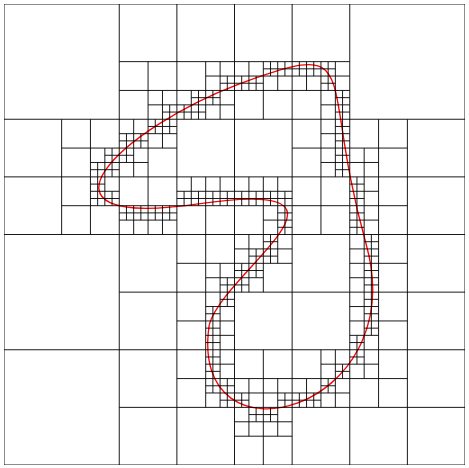
\includegraphics[width=0.5\textwidth]{figures/terrain_subdivision_for_road}
    \caption{Podział terenu w celu optymalizacji ilości obliczeń}
    \label{fig}
\end{figure}

\section{Dodanie obiektów}
Ostatnim etapem jest dodanie obiektów, takich jak meta oraz pojazdy. Domyślnie na każdym torze znajdą się cztery pojazdy, ustawione jeden za drugim, z czego trzy sterowane przez bota, a jeden przez gracza. Dodatkowo dodawane są krawędzie, których celem jest zapobieganie spadania pojazdu poza wygenerowany teren. W celu śledzenia przebiegu trasy, w równych odstępach dodawane są punkty kontrolne.\\
Przykładowo otrzymano poniższy efekt:
\begin{figure}[h]
    \minipage{.5\textwidth}
        \centering
        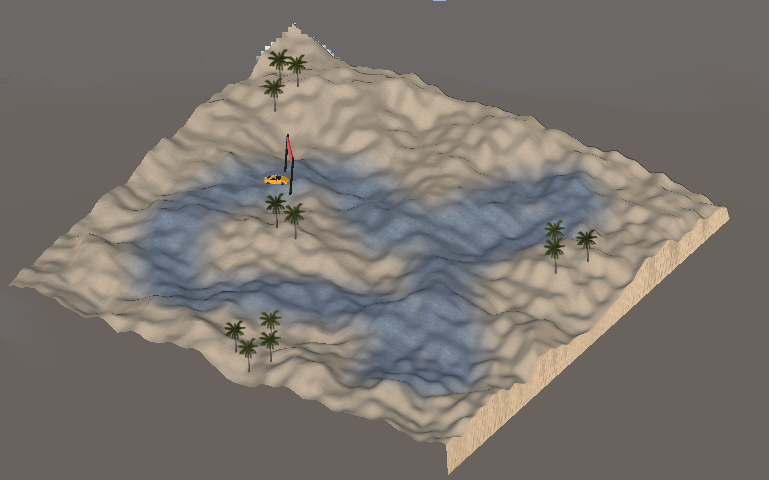
\includegraphics[height=5cm]{figures/terrains_2.png}
    \endminipage\hfill
    \minipage{.5\textwidth}
        \centering
        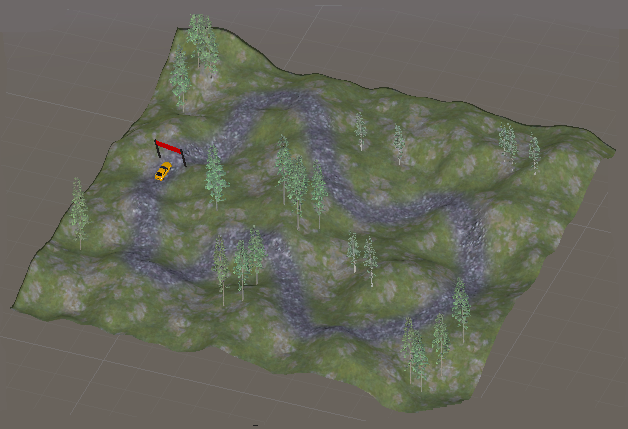
\includegraphics[height=5cm]{figures/terrains_1.png}
    \endminipage
    \caption{Wygenerowane tereny}
    \label{table}
\end{figure}
\clearpage
	\clearpage % \cleardoublepage

	\chapter{Wytrenowanie bota}
\thispagestyle{chapterBeginStyle}

\section{Cel i funkcjonalności}
Wytrenowany bot powinien być w stanie poruszać się po wygenerowanym wcześniej terenie, rozpoznając i trzymając się drogi. Trening bota powinien wykorzystywać metody uczenia przez wzmacnianie.

\section{Wykorzystane technologie}
Silnik Unity udostępnia dodatek open-source ML-Agents \cite{UnityMlAgentsRepository} \cite{UnityMlAgents}, który pozwala na wykorzystanie środowisk utworzonych w grze do treningu modeli. Stanowi on warstwę łączącą Unity z biblioteką Tensorflow, oraz zapewnia wiele nowoczesnych algorytmów głębokiego uczenia przez wzmacnianie (m.in. Proximal Policy Optimization (PPO), Soft Actor-Critic (SAC), self-play). W powyższej pracy wykorzystano algorytm PPO, ze względu na większą stabilność treningu \cite{CompareDrlAlgorithms}. Śledzenie wielu metryk postępu uczenia było dostępnych z wykorzystaniem programu tensorboard.

\section{Uczenie przez wzmacnianie}
Uczenie przez wzmacnianie jestem jednym z trzech głównych nurtów uczenia maszynowego, gdzie agent uczy się polityki optymalnej w danym środowisku metodą prób i błędów, otrzymując wyłącznie wartość nagrody jako informację zwrotną. W przeciwieństwie do uczenia nadzorowanego, metoda ta nie wymaga wcześniejszego przygotowania dużej ilości opisanych danych. Pozwala to na wprowadzenie bota do nieznanego środowiska i natychmiastowe podjęcie interakcji.\\
Cykl uczenia przez wzmacnianie opiera się na akcji bota i reakcji. Bot zbiera obserwacje na podstawie stanu w jakim się znajduje w środowisku. Następnie podejmuje decyzję na podstawie obserwacji. Po podjęciu decyzji wykonywana jest odpowiednia akcja, po czym za akcję przyznawana jest nagroda lub kara, w zależności czy akcja wpłynęła pozytywnie na przybliżanie się bota do celu. Na podstawie zbioru informacji zawierającego stan początkowy, podjęte akcje i otrzymaną nagrodę trenowana jest polityka, maksymalizując oczekiwaną nagrodę.
\clearpage
\section{Metodyka uczenia}
Wstępne uczenie odbywa się na terenach płaskich (wysokość każdego punktu jest równa zero) oraz w terenie ze zwiększonym kontrastem - droga jest czarna a wszystko pozostałe jest białe. Do treningu uruchomione jest naraz 12 terenów, zawierających 4 różne trasy. Na każdym z terenów znajduje się pomiędzy 1 a 4 pojazdy, co oznacza że model jest trenowany na 12-48 niezależnych instancjach naraz, w celu przyspieszenia nauki. W kolejnych etapach zwiększany jest stopień trudności trasy, reprezentowany przez ilość i ostrość zakrętów. Następnie zwiększane jest pofałdowanie terenu, oraz zmieniane są tekstury drogi i terenu.
\begin{figure}[H]
    \centering
    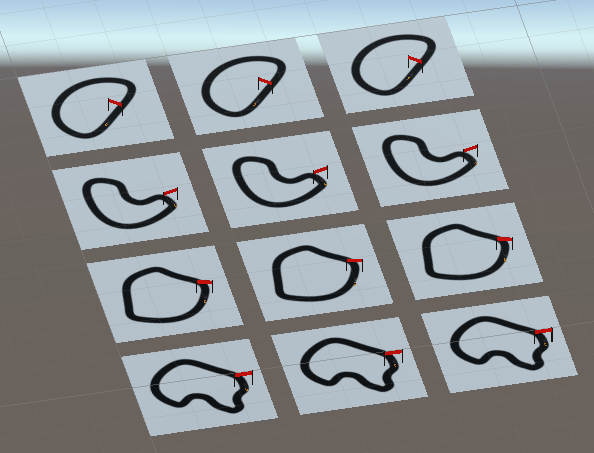
\includegraphics[width=.5\textwidth]{figures/multiple_tests}
    \caption{Prowadzenie wielu treningów na raz}
    \label{fig}
\end{figure}

\section{Analiza wyników}
Wyniki uczenia przedstawione zostały na wykresie za pomocą dwóch metryk. Wartość \textit{Cumulative Reward} oznacza średnią wartość nagrody z jednego epizodu dla jednego agenta. Wartosć \textit{Visited punkt kontrolnys} informuje jak dużą część trasy przeszedł agent, uśrednioną z jednego epizodu dla jednego agenta. Pełne okrążenie zaweira w sobie 40 punktów kontrolnych. Wartości zaznaczone na wykresach bledszym kolorem są wartościami rzeczywistymi, natomiast wartości pogrubione wyliczone zostały z wykorzystaniem średniej kroczącej eksponencjalnej, aby lepiej uwidocznić tendencje zmian.

\begin{figure}[H]
    \centering
    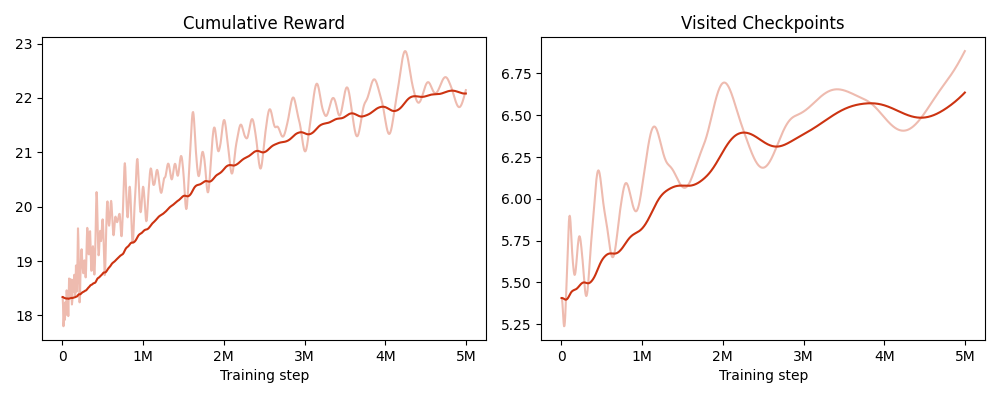
\includegraphics[width=\textwidth]{graphs/example}
    \caption{Przykładowa analiza wyników}
    \label{fig}
\end{figure}

\subsection{Wybór obserwacji}
Wybór informacji, jakie dostępne są dla bota znacznie wpłynie na podejmowane przez niego decyzje. Za mała ilość informacji nie pozwoli na wykrycie odpowiedniej ilości szczegółów trasy, natomiast za duża znacznie zwiększy czas treningu i inferencji, wprowadzając niepotrzebny szum.

\subsubsection{Dane wynikające z trasy}
Pierwszy sposób obserwacji opiera się na wartościach, do których zwykły gracz nie ma dostępu, ponieważ wymagają m.in. znajomości dokładnego wzoru  krzywej trasy do wyliczenia. Dane, które są przekazywane do modelu jako obserwacje to:
\begin{itemize}
    \item odległość w linii prostej od aktualnej pozycji do centrum szerokości trasy
    \item kąt pomiędzy kierunkiem jazdy pojazdu a kierunkiem stycznej do toru
    \item odległość w linii prostej od aktualnej pozycji do najbliższego punktu kontrolnego
    \item kąt pomiędzy kierunkiem jazdy pojazdu a kierunkiem do najbliższego punktu kontrolnego
    \item kąt nachylenia terenu
    \item aktualna pozycja kół ($-1$ oznacza maksymalnie skręcone w lewo, $1$ maksymalnie w prawo)
    \item aktualny stopień wciśnięcia pedału gazu ($-1$ oznacza jazdę do tyłu, $1$ jazdę do przodu)
    \item aktualna prędkość
\end{itemize}

\subsubsection{Dane odległości od krawędzi}
Podobnie jak większość samochodów autonomicznych, poniższa metoda wykorzystuje wizualizację przestrzeni na podstawie odległości, nazywaną lidar \cite{Lidar}. Technologia ta w realnym świecie buduje model otoczenia wysyłając wiązki laserowe i mierząc trasę przebytą przez nie do przeszkody. Analogicznie, symulowany pojazd testuje odległości od krawędzi trasy oraz ewentualnych przeszkód, takich jak inne pojazdy.
\begin{figure}[H]
    \centering
    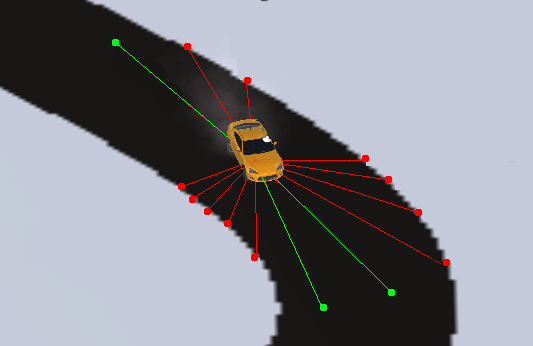
\includegraphics[width=.5\textwidth]{figures/observations_0}
    \caption{Obserwacje bota dystansów na około pojazdu}
    \label{fig}
\end{figure}
Dodatkowo przekazywana jest aktualna prędkość pojazdu jako obserwacja, zważywszy że nie da się jej w żaden sposób odczytać z jednej klatki pomiarów.

\subsubsection{Dane wizualne jednowymiarowe}
Poniższe podejście testuje metodę obserwacji wykorzystującą bodźce wizualne. W tym przypadku tworzona jest lista wartości kolorów dla każdego punktu w stałej odległości od pojazdu. Generuje to okrąg kolorów na około pojazdu, który powinien być w stanie przekazać takie informacje jak zakręty na trasie, będąc znacznie mniejszego rozmiaru niż obraz z kamery. Na rysunku zaznaczono kilka promieni pobierających kolory otoczenia.
\begin{figure}[H]
    \centering
    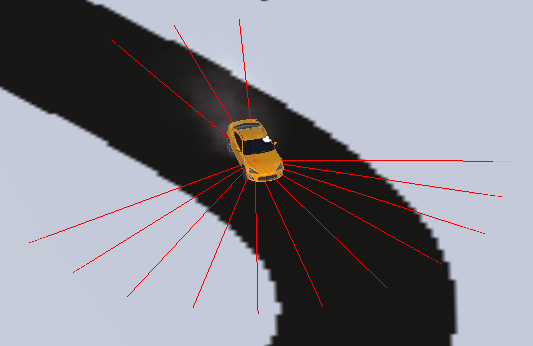
\includegraphics[width=.5\textwidth]{figures/observations_1}
    \caption{Obserwacje bota kolorów na około pojazdu}
    \label{fig}
\end{figure}
Dodatkowo przekazywana jest aktualna prędkość pojazdu jako obserwacja, zważywszy że nie da się jej w żaden sposób odczytać z danych wizualnych.

\subsubsection{Dane wizualne z kamery przedniej}
Wykorzystująć imformacje w postaci w jakiej są one widoczne dla każdego gracza, kolejna metoda pobiera obraz z kamery jako obserwacje. Kamera umiejscowiona jest na przedzie pojazdu, zapewniając perspektywę podobną do zwykłego prowadzenia auta. Aby ograniczyć ilość informacji dostarczanych do sieci, obraz z kamery skalowany jest do rozdzielczości $40x20$ oraz konwertowany na skalę szarości. Dodatkowo, jak powyżej, przekazywana jest aktualna prędkość pojazdu.
\begin{figure}[H]
    \centering
    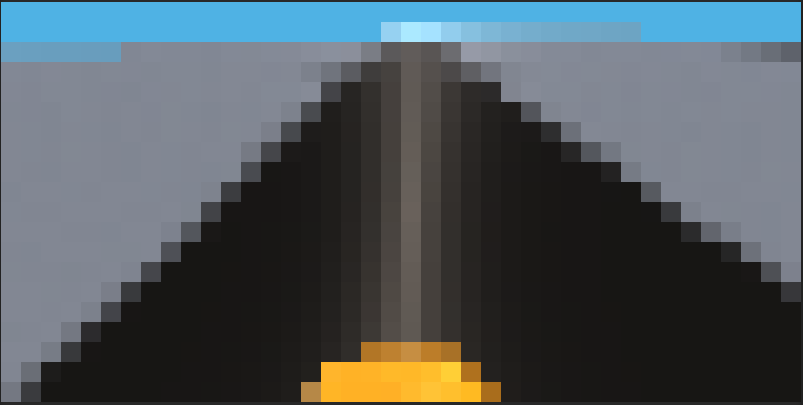
\includegraphics[width=.5\textwidth]{figures/observations_2}
    \caption{Obserwacje bota z kamery przedniej}
    \label{fig}
\end{figure}

\subsubsection{Dane wizualne z kamery z lotu ptaka}
Wykorzystująć imformacje widoczne przez kamerę z lotu ptaka model powinien być w stanie łatwiej zauważyć krzywiznę toru. Tak jak powyżej, obraz z kamery skalowany jest do rozdzielczości $30x20$ oraz konwertowany na skalę szarości, oraz przekazywana jest aktualna prędkość pojazdu.
\begin{figure}[H]
    \centering
    
\includegraphics[width=.5\textwidth]{figures/observations_3}
    \caption{Obserwacje bota z kamery z lotu ptaka}
    \label{fig}
\end{figure}

\subsubsection{Porównanie}
Poniżej znajdują się wykresy porównujące szybkość uczenia się w pierwszych 400 000 iteracjach. Wykres pierwszy pokazuje otrzymaną nagrodę za akcję, uśrednioną dla każdego agenta, dla każdej akcji. Drugi wykres przedstawia jak daleko udało się dojechać. Na przestrzeni całego toru rozłożone jest 40 punktów kontrolnych. Celem jest maksymalizacja obu wartości.
\begin{figure}[H]
    \centering
    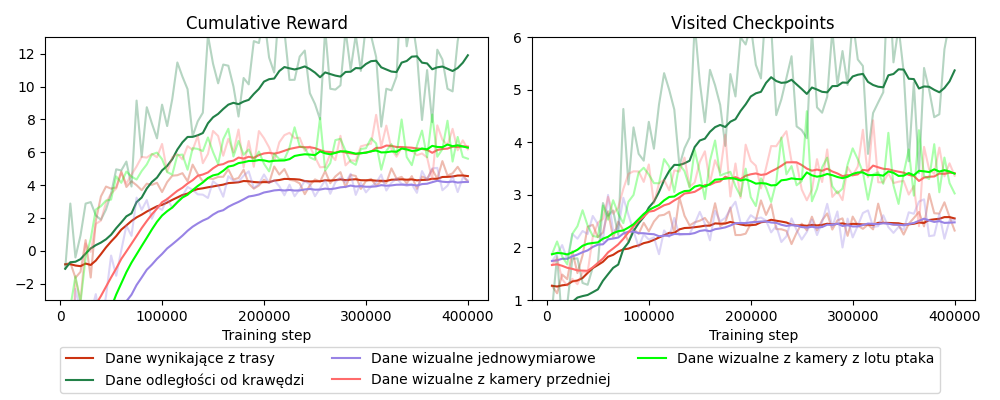
\includegraphics[width=\textwidth]{graphs/input_observations}
    \caption{Porównanie metod obserwacji}
    \label{fig}
\end{figure}
Najlepsze wyniki otrzymano dla metody wykorzystującej odległości od przeszkód. Metoda ta zbiera łącznie 14 dystansów, co wystarcza do zawarcia najpotrzebniejszych informacji. Dane z kamery okazały się zbyt obszerne (odpowiednio 600 i 800 pikseli), spowalniając trening.
\clearpage
\subsection{Wybór akcji}
Po podjęciu decyzji bot musi wykonać odpowiednią akcję. Bot podejmuje decyzję w dwóch płaszczyznach. Pierwsza odnosi się do przemieszczania przód-tył, natomiast dróga odpowiada skręceniu kierownicy prawo-lewo. Decyzje te mogłyby być wybierane z przestrzeni ciągłych lub dyskretnych.

\subsubsection{Akcje w przestrzeni ciągłej}
Dla każdej płaszczyzny bot zwraca wartość rzeczywistą z zakresu $[-1, 1]$. W pierwszej płaszczyźnie wartość odpowiada dokładnie stopniowi wciśnięcia pedału gazu, natomiast w drugiej - kątowi skrętu kierownicy. Poniważ bot jest w stanie zawsze ustawić konkretną wartość, przejścia pomiędzy kolejnymi akcjami nie muszą być płynne - w pierwszej klatce bot może skierować kierownicę 30 stopni w lewo, natomaist już klatkę później może ustawić ją na 20 stopni w prawo, bez stanów przejściowych.

\subsubsection{Akcje w przestrzeni dyskretnej}
Dla każdej płaszczyzny bot zwraca wartość całkowita ze zbioru ${-1, 0, 1}$. W pierwszej płaszczyźnie wartość $-1$ odpowiada zwiększeniu nacisku na pedał hamulca, $0$ oznacza brak zmian, $1$ oznacza zwiększenie nacisku na pedał gazu. Analogicznie w drugiej plaszczyźnie, $-1$ odpowiada skręceniu kierownicy mozniej w lewo, $1$ mocniej w prawo, a $0$ brak zmian. W ten sposób zmiany są bardziej płynne w czasie.

\subsubsection{Porównanie}
Zastosowanie akcji dyskretnych pozwoliło botowi na zancznie łatwiejsze poruszanie się w środowisku, co przełożyło sie na znacznie lepsze wyniki w pierwszych 300 000 krokach treningu.
\begin{center}
    \color[HTML]{CC3311} ------------ \color{black} Akcje ciągłe \hspace{1cm} \color[HTML]{0077BB} ------------ \color{black} Akcje dyskretne
\end{center}
\begin{figure}[H]
    \centering
    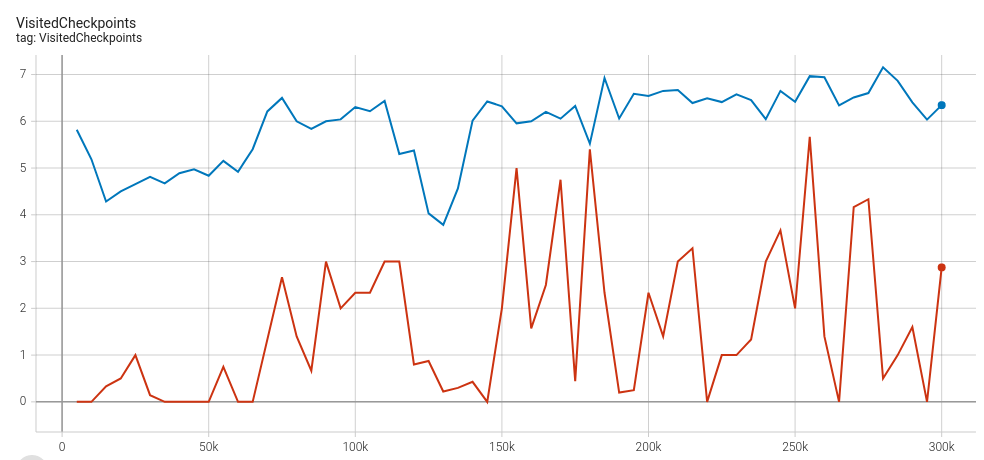
\includegraphics[width=.5\textwidth]{figures/output_values_compare}
    \caption{Porównanie metod podejmowania akcji}
    \label{fig}
\end{figure}

\section{Zdefiniowanie funkcji oceny}
Ocena powinna odzwierciedlać w jakim stopniu wykonana akcja przybliżyła bota do osiągnięcia celu. W każdym cyklu, podjęta akcja oceniana jest na podstawie trzech parametrów.
\begin{align*}
    Q &= (0.5 - distanceToRoadCenter) \cdot 0.1 + \\
    & (0.05 - abs(angleToTangent)) + \\
    & (distanceTraveledInFrame - 0.1) + \\
    & 0.01
\end{align*}
Po pierwsze przyznawana jest nagroda za utrzymywanie sie w odległości mniejszej niż 50\% szerokości drogi od środka drogi (linia czerwona na poniższym rysunku), w przeciwnym przypadku kara, wprost proporcjonalna do ww. odległości. Po drugie przyznawana jest nagroda za utrzymywanie kierunku jazdy (linia zielona na poniższym rysunku) w zakresie $\pm10$ stopni od kierunku trasy (linia niebieska na poniższym rysunku), w przeciwnym przypadku kara, wprost proporcjonalna do w.w kąta. Po trzecie przyznawana jest nagroda za dystans pokonany od ostatniej akcji, jeżeli wynosi co najmniej $0.1$. Dodatkowo przyznawana jest nagroda za każdą klatkę, aby promować jak najdłuższe treningi.
\begin{figure}[H]
    \centering
    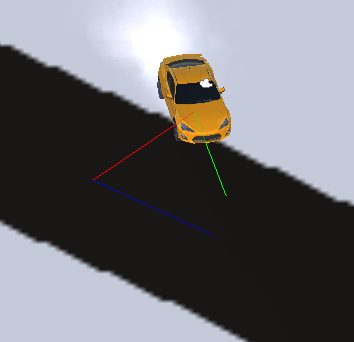
\includegraphics[width=.5\textwidth]{figures/rewards}
    \caption{Wizualizacja oceny akcji}
    \label{fig}
\end{figure}
Dodatkowo bot oceniany jest za każdym razem kiedy wejdzie w interakcję z innym obiektem. Na około całego terenu rozmieszczone są bariery, które powodują koniec epizodu po dotknięciu i powrót pojazdu na pozycję początkową, dodatkowo dodając karę $0.1$. Na pierwszym etapie treningu takie same bariery ustawione są wzdłuż drogi, tak że pojazd kończy epizod za każdym razem kiedy zjedzie z drogi. Po wytrenowaniu bota w takich warunkach bariery te zostaną ściągnięte, aby zobaczyć czy mimo to bot będzie trzymał sie drogi.\\
Wzdłuż całej trasy rozstawione są punkty kontrolne, które pojazd powinien przebyć w odpowiedniej kolejności. Za każdy punkt kontrolny zaliczony w kolejności nagroda zwiększa się o $1$. Jeżeli pojazd zahaczy o któryś z 4 sąsiednich punktów kontrolnych (2 w tył, 2 w przód) dostaje tylko karę $0.1$, natomiast jeżeli dotknie innego punktu kontrolnego, epizod jest kończony z karą $-1$.
\begin{figure}[H]
    \centering
    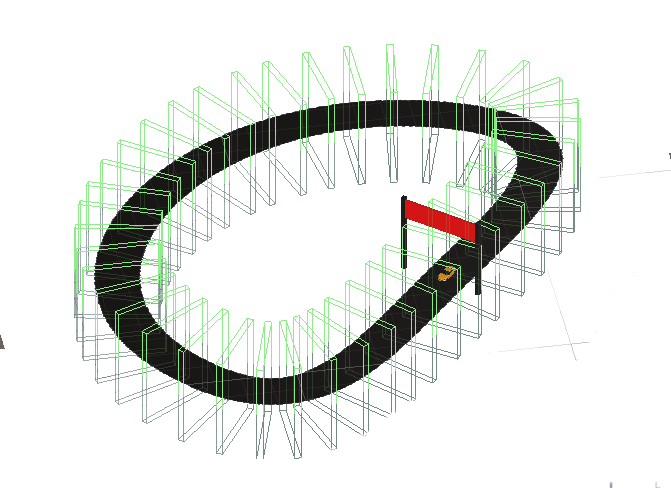
\includegraphics[width=.5\textwidth]{figures/checkpoints}
    \caption{Rozmieszczenie punktów kontrolnych}
    \label{fig}
\end{figure}

\section{Dobranie parametrów}
Wybrany algorytm Proximal Policy Optimization pozwala na osiągnięcie nie najgorszych wyników, natomiast dostosowanie hyperparametrów potrafi znacznie poprawić efekty treningu.
\\\\
\begin{algorithm}[H]
\caption{Hiperparametry początkowe treningu}\label{alg}
$hyperparameters:$\\
    \hskip2em $batch\_size: 1024$\\
    \hskip2em $buffer\_size: 10240$\\
    \hskip2em $learning\_rate: 0.0003$\\
    \hskip2em $beta: 0.005$\\
    \hskip2em $epsilon: 0.2$\\
    \hskip2em $lambd: 0.95$\\
    \hskip2em $num\_epoch: 3$\\
    \hskip2em $learning\_rate\_schedule: linear$\\
% $network\_settings:$\\
%     \hskip2em $normalize: False$\\
%     \hskip2em $hidden\_units: 128$\\
%     \hskip2em $num\_layers: 2$\\
%     \hskip2em $vis\_encode\_type: simple$\\
%     \hskip2em $memory: None$\\
%     \hskip2em $goal\_conditioning\_type: hyper$\\
$reward\_signals:$\\
    \hskip2em $extrinsic:$\\
        \hskip4em $gamma: 0.99$\\
        \hskip4em $strength: 1.0$\\
\end{algorithm}
\phantom{.}\\
Poniżej zostały przedstawione wybory poszczególnych parametrów. Porównane zostały konfiguracje dla pierwszych $500 000$ iteracji, za każdym razem zaczynając od losowych wag. Po wyborze optymalnej wartości parametru, była ona aktualizowana i wykorzystywana w kolejnych testach jako domyślna.\\
\clearpage

\subsection{gamma}
Parametr $gamma$ można rozumieć jako jak daleko w przyszłość agent powinien dbać o możliwe nagrody. W sytuacjach gdy agent powinien podejmować decyzje w oczekiwaniu na przewidywane nagrody w przyszłości, wartość $gamma$ powinna być większa ($0.995$), natomiast jeżeli agent powinien bardziej dbać o nagrody natychmiastowe wartość $gamma$ może osiągać niższe wartości ($0.8$). Po porównaniu granic typowego zakresu wartości, na wykresach poniżej widać, że wartość niższa przekłada się na minimalnie lepszy trening.
\begin{figure}[H]
    \centering
    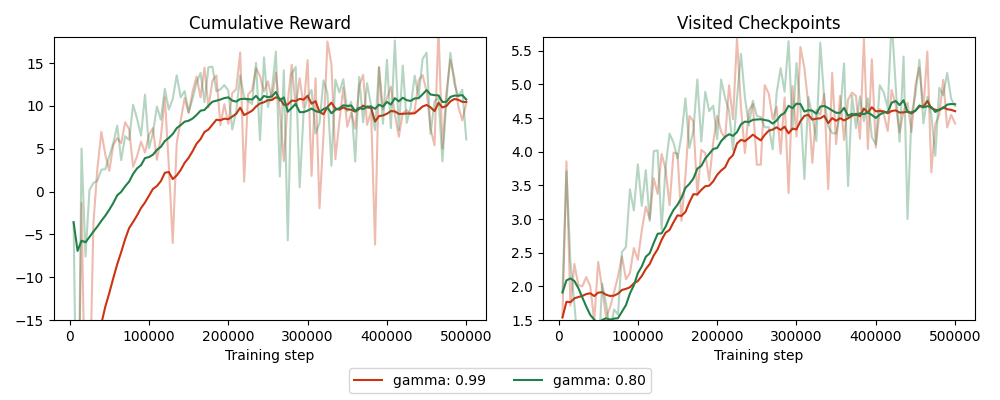
\includegraphics[width=\textwidth]{graphs/hyperparameters_gamma.png}
    \caption{Wybór hiperparametrów: gamma}
    \label{fig}
\end{figure}

\subsection{lambda}
Parametr $lambda$ definiuje w jakim stopniu agent polega na przewidzianej wartości podczas przewidywania kolejnej wartości. Niższe wartości $lambda$ oznaczają poleganie w większym stopniu na przewidzianej wartości, natomiast większa $lambda$ odpowiada poleganiu bardziej na rzeczywiście otrzymanych nagrodach. Po porównaniu granic typowego zakresu wartości ($0.85-0.95$), na wykresach poniżej widać, że wartość niższa przekłada się na minimalnie lepszy trening.
\begin{figure}[H]
    \centering
    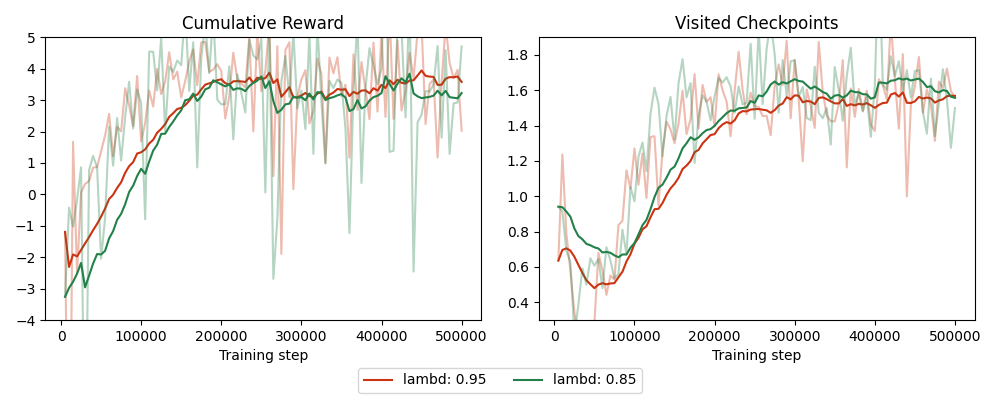
\includegraphics[width=\textwidth]{graphs/hyperparameters_lambd.png}
    \caption{Wybór hiperparametrów: lambd}
    \label{fig}
\end{figure}

\subsection{buffer size}
Rozmiar bufora odpowiada ilości cykli treningowych (zebranie obserwacji, podjęcie akcji, otrzymanie nagrody) które są zbierane przed aktualizacją modelu. Większa wartość przekłada się na bardziej stabilny trening, kosztem czasu. Po porównaniu wartości $10240$ i $40960$ można zauważyć, że niższa wartość zapewnia zadowalającą stabilność, otrzymując podobne wartości znacznie wcześniej.
\begin{figure}[H]
    \centering
    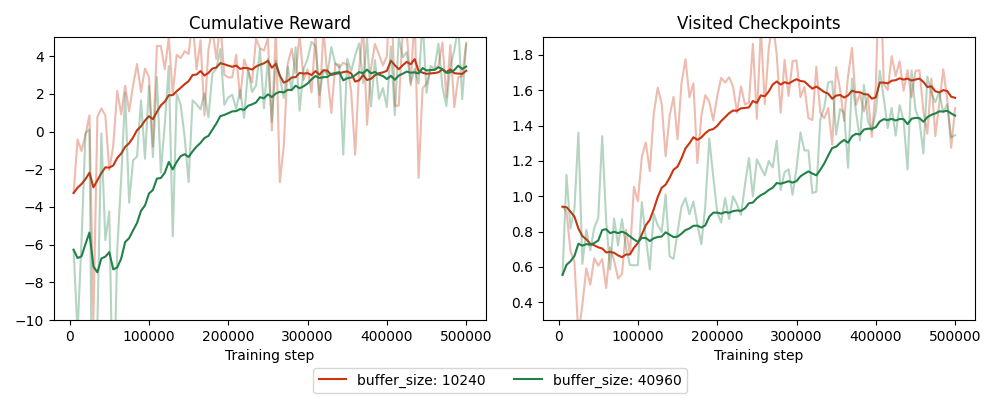
\includegraphics[width=\textwidth]{graphs/hyperparameters_buffer_size.png}
    \caption{Wybór hiperparametrów: buffer size}
    \label{fig}
\end{figure}

\subsection{batch size}
Parametr $batch\_size$ definiuje ilość cykli treningowych wykorzystywanych przy propagacji wstecznej. Przy dyskretnej przestrzeni akcji wartość ta powinna być mniejsza, niż dla akcji ciągłych. Zmniejszenie $batch\_size$ do $256$ minimalnie poprawiło trening, natomiast spadek do $32$ nie wprowadził zauważalnych różnic.
\begin{figure}[H]
    \centering
    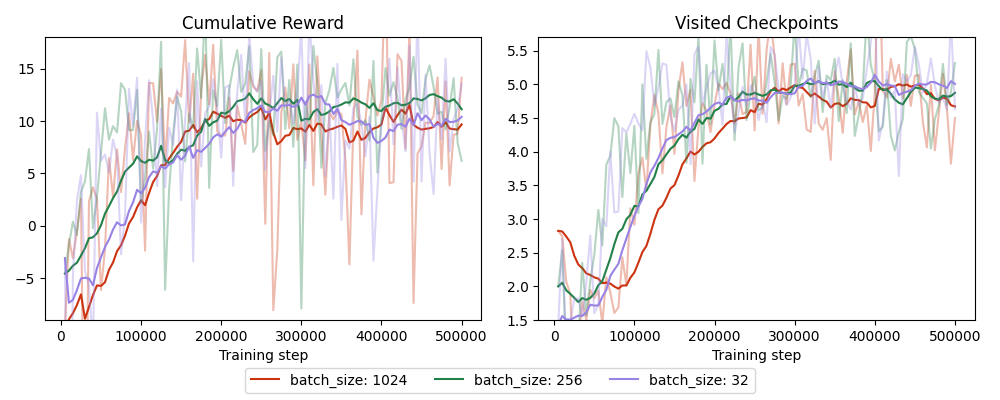
\includegraphics[width=\textwidth]{graphs/hyperparameters_batch_size.png}
    \caption{Wybór hiperparametrów: batch size}
    \label{fig}
\end{figure}
\clearpage

\subsection{learning rate}
Prędkość uczenia bezpośrednio odnosi się do siły każdego kroku propagacji wstecznej. Analizując poniższe wykresy, wartość pośrodku typowego zakresu ($1e-3, 1e-5$) pozwala na najbardziej optymalną prędkość uczenia w skali 500000 iteracji.
\begin{figure}[H]
    \centering
    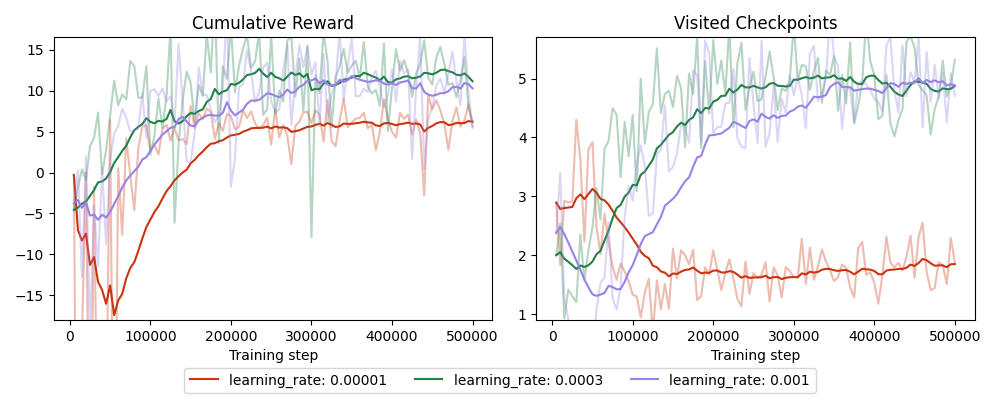
\includegraphics[width=\textwidth]{graphs/hyperparameters_learning_rate.png}
    \caption{Wybór hiperparametrów: learning rate}
    \label{fig}
\end{figure}

\subsection{beta}
Parametr $beta$ definiuje skalę randomizacji polityki. Większe wartości parametru powodują podejmowanie przez bota większej ilości losowych akcji, zwiększając ilość sprawdzanych rozwiązań. Dla zadanego problemu niższa $beta$ powoduje szybsze unormowanie się wartości nagrody oraz postępu trasy, dlatego została wybrana wartość $0.005$.
\begin{figure}[H]
    \centering
    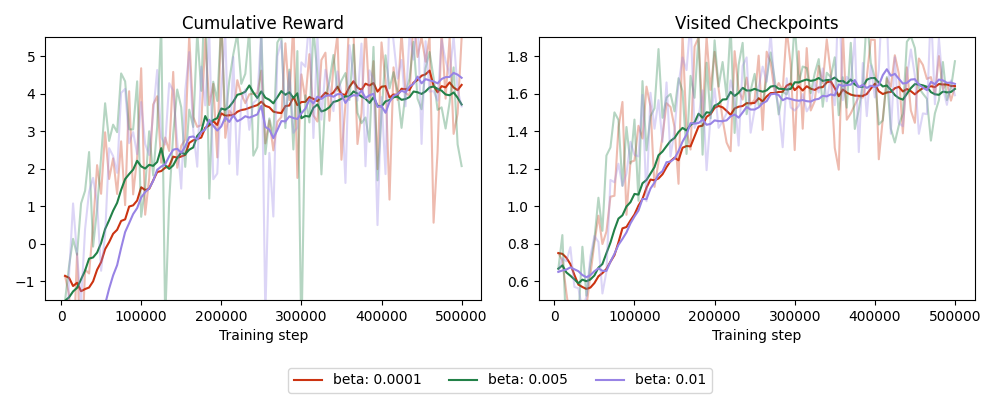
\includegraphics[width=\textwidth]{graphs/hyperparameters_beta.png}
    \caption{Wybór hiperparametrów: beta}
    \label{fig}
\end{figure}
\clearpage

\subsection{epsilon}
Zmienna $epsilon$ informuje w jakim stopniu akceptowane są rozbieżności pomiędzy starą i nową polityką podczas propagacji wstecznej. Niższe wartości powodują bardziej stabilny postęp kosztem czasu treningu. Zwiększenie wartości do $0.4$ nie spowodowało jednak przyspieszenia treningu.
\begin{figure}[H]
    \centering
    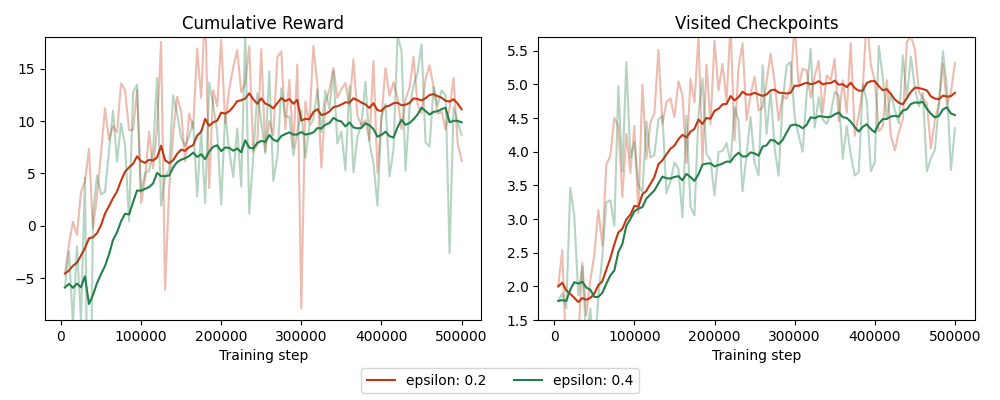
\includegraphics[width=\textwidth]{graphs/hyperparameters_epsilon.png}
    \caption{Wybór hiperparametrów: epsilon}
    \label{fig}
\end{figure}

% \subsection{visual encode type}
% Ponieważ agent korzysta z danych wizualnych z kamery, są one procesowane przez konwolucyjną sieć neuronową. Poniżej zostały porównane trzy rodzaje sieci konwolucyjnych z prostą siecią łączącą wszystkie wejścia z wszystkimi wyjściami (\textit{fully connected}). Sieć $simple$ składa się tylko z dwóch warstw konwolucyjnych. Sieć $resnet$ wykorzystuje znacznie większą implementację IMPALA Resnet \cite{ImpalaResnet}. Sieć $match3$ \cite{Match3} jest mniejszą siecią konwolucyjną zoptymalizowaną dla gier planszowych i o segmentowym układzie, co dobrze reaguje na wykorzystanie kamery niskiej rozdzielczości, gdzie każdemu pikselowi odpowiada komórka gry.
% \begin{figure}[H]
%     \centering
%     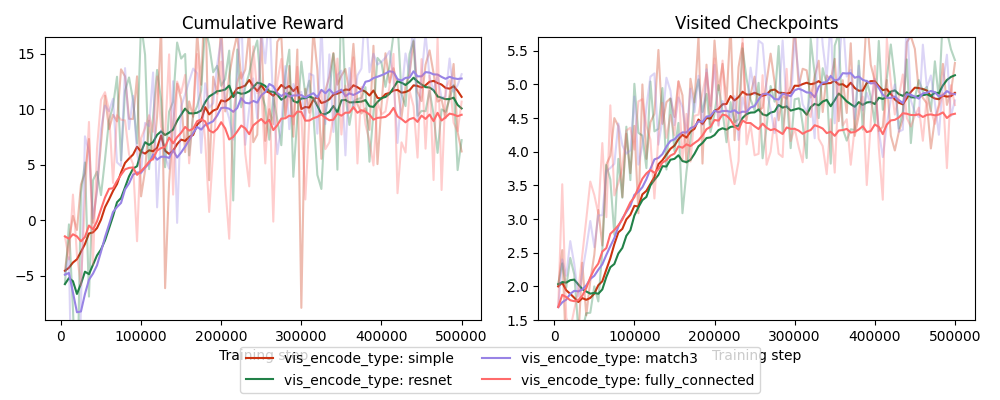
\includegraphics[width=\textwidth]{graphs/hyperparameters_vis_encode_type.png}
%     \caption{Wybór hiperparametrów: vis encode type}
%     \label{fig}
% \end{figure}

% \subsection{network size}
% \begin{figure}[H]
    %     \centering
    %     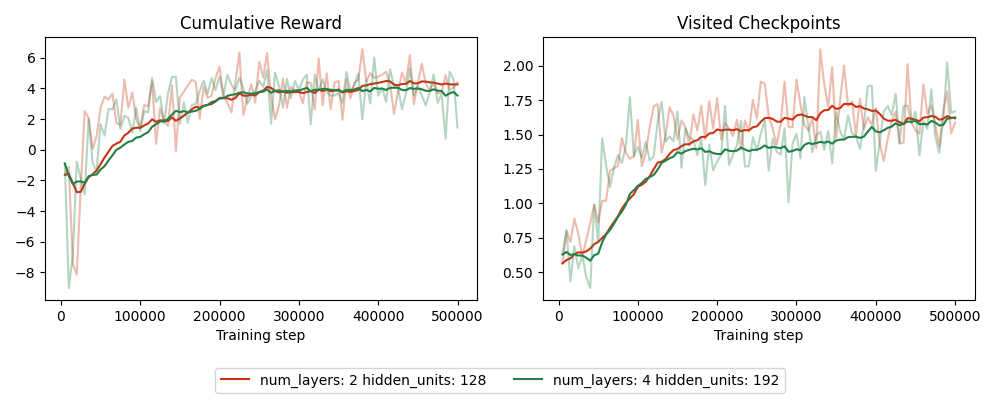
\includegraphics[width=\textwidth]{graphs/hyperparameters_network_size.png}
    %     \caption{Wybór hiperparametrów: layers, hidden units}
    %     \label{fig}
    % \end{figure}

Finalnie zostały wybrane poniższe hiperparametry, co pozwoliło na zauważalną poprawę treningu. Średnia wartość nagrody dla całego okresu wzrosła z $2.46$ do $3.26$ ($+32.5\%$), natomaist stopień postępu trasy wzrósł z $1.305$ do $1.499$ ($+14.9\%$).
\begin{figure}[H]
    \centering
    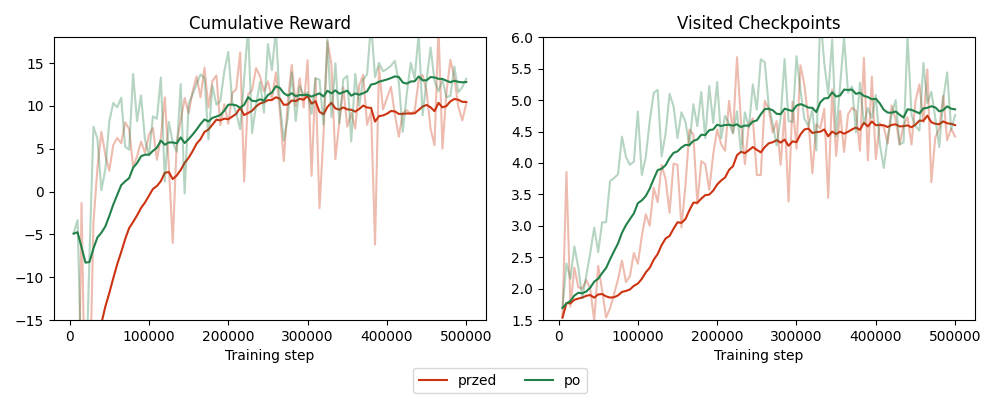
\includegraphics[width=\textwidth]{graphs/hyperparameters_tuning_results.png}
    \caption{Wybór hiperparametrów: porównanie wyników}
    \label{fig}
\end{figure}
\begin{algorithm}[H]
\caption{Hiperparametry finalne treningu}\label{alg}
$hyperparameters:$\\
    \hskip2em $batch\_size: 256$\\
    \hskip2em $buffer\_size: 10240$\\
    \hskip2em $learning\_rate: 0.0003$\\
    \hskip2em $beta: 0.005$\\
    \hskip2em $epsilon: 0.2$\\
    \hskip2em $lambd: 0.85$\\
    \hskip2em $num\_epoch: 8$\\
    \hskip2em $learning\_rate\_schedule: linear$\\
% $network\_settings:$\\
%     \hskip2em $normalize: False$\\
%     \hskip2em $hidden\_units: 128$\\
%     \hskip2em $num\_layers: 2$\\
%     \hskip2em $vis\_encode\_type: match3$\\
%     \hskip2em $memory: None$\\
%     \hskip2em $goal\_conditioning\_type: hyper$\\
$reward\_signals:$\\
    \hskip2em $extrinsic:$\\
        \hskip4em $gamma: 0.8$\\
        \hskip4em $strength: 1.0$\\
\end{algorithm}
\clearpage
\section{Dalsze etapy treningu}
Przy trenowaniu ważne jest, aby początkowe zadania były proste, aby agent był w stanie je łatwo wykonać. Następnie należy stopniowo zwiększać poziom trudności, dając agentowi odpowiednio dużo czasu na przystosowanie się do zmian. Dlatego pierwszy etap treningu polega na przejechaniu trasy będącej okręgiem, po płaskim terenie, bez wykorzystania tekstur (droga jest czarna, otoczenie białe) oraz bez przeciwników (w każdym środowisku znajduje się jeden agent).
\begin{figure}[H]
    \centering
    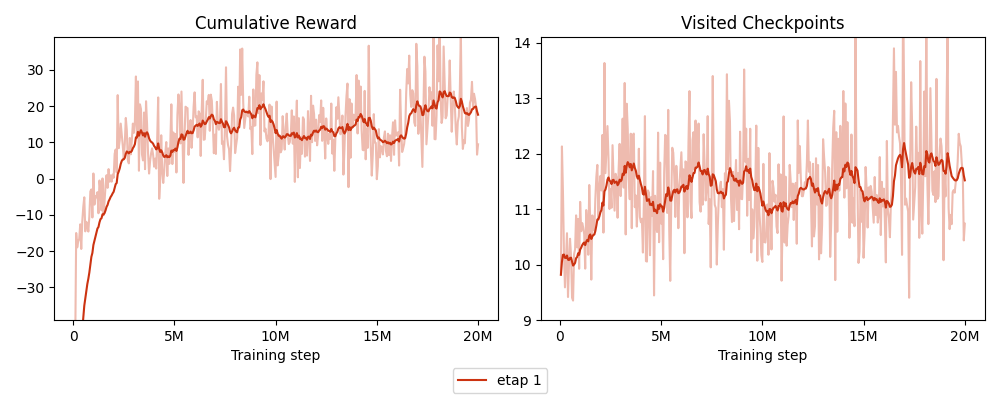
\includegraphics[width=\textwidth]{graphs/training_progress_1.png}
    \caption{Postep treningu: etap 1}
    \label{fig}
\end{figure}
\phantom{.}\\
Etap 2 zakłada dodanie większej różnorodności torów, zachowując stosunkowo prosty kształt, tylko nieznacznie odbiegający od okręgu, z małą ilością ostrych zakrętów.\\
% \textbf{TODO wykres postępu}\\
Etap 3 sprawdza adaptowalność pojazdu na skomplikowanym torze, z dużą ilością ostrych zakrętów.\\
% \textbf{TODO wykres postępu}\\
Etap 4 zakłada dodanie nierówności terenu, tworząc góry i pagórki na trasie.\\
% \textbf{TODO wykres postępu}\\

	\clearpage % \cleardoublepage
	
	\chapter*{Podsumowanie}
\addcontentsline{toc}{chapter}{Podsumowanie}
\thispagestyle{chapterBeginStyle}
W powyższej pracy została stworzona gra wyścigowa, wraz z botem. Bot został wytrenowany z wykorzystaniem uczenia przez wzmacnianie przy pomocy Unity ML-Agents. Jako interakcję ze środowiskiem bot posiada do dystpozycji dwie akcje w przestrzeni dyskretnej o wartościach {-1, 0, 1} definiujące poruszanie się do przodu/tyłu oraz kąt skrętu kierownicy. Pojazd porusza się zgodnie z uproszczonymi zasadami fizyki symulowanymi przez silnik Unity. Jako obserwacje przyjmuje odległości pojazdu od ewentualnych przeszkód oraz krawędzi drogi i aktualną prędkość. Taki zbiór danych wejściowych ma na celu symulować podejście wykorzystywane aktualnie w samochodach autonomicznych.

Proces implementacji bota, wraz z wyborem obserwacji, podejmowanych akcji, funkcji nagrody i wyboru hiperparametrów przedstawiony został na wykresach ilustrujących efekty podjętej decyzji. W pracy zostały również opisane kolejne etapy treningu bota.

	\clearpage % \cleardoublepage
	
	
	%%%%%%%%%%%%%%%%%%%%%%%%%%%%%%%%%%%%%%%%%%%%%%%%%%%%%%%%%%%%%%%%%%%%%%%%%%%%%%
	%%%%%%%%%%%%%%%%%%%%%%%%%%%%%%% BIBLIOGRAFIA %%%%%%%%%%%%%%%%%%%%%%%%%%%%%%%%%
	%%%%%%%%%%%%%%%%%%%%%%%%%%%%%%%%%%%%%%%%%%%%%%%%%%%%%%%%%%%%%%%%%%%%%%%%%%%%%%

	\pagestyle{bibliographyStyle}
	\bibliographystyle{plainurl}
	% \bibliographystyle{plabbrv}
	\bibliography{literatura}
	\thispagestyle{chapterBeginStyle}
        \addcontentsline{toc}{chapter}{Bibliografia}
	\clearpage % \cleardoublepage
	
	%%%%%%%%%%%%%%%%%%%%%%%%%%%%%%%%%%%%%%%%%%%%%%%%%%%%%%%%%%%%%%%%%%%%%%%%%%%%%%
	%%%%%%%%%%%%%%%%%%%%%%%%%%%%%%%%% DODATKI %%%%%%%%%%%%%%%%%%%%%%%%%%%%%%%%%%%%
	%%%%%%%%%%%%%%%%%%%%%%%%%%%%%%%%%%%%%%%%%%%%%%%%%%%%%%%%%%%%%%%%%%%%%%%%%%%%%%
	
	\appendix
	\pagestyle{appendixStyle}
       \renewcommand{\appendixname}{Załącznik}
	
	\chapter{Uruchomienie gry}
\thispagestyle{chapterBeginStyle}

Kod źródłowy programu, wraz z plikami wykonywalnymi gry, znajduje się na załączonej płycie CD, oraz online w repozytorium GitHub \cite{Github}.

\section{Struktura plików}
Struktura plików wygląda następująco:\\
\begin{algorithm}[H]
    $./$\\
    $|\textit{| Kod\_Źródłowy/}$\\
    $|\hskip2em |\textit{| Assets/}$\\
    $|$\\
    $|\textit{| Gra/}$\\
    $|\hskip2em |\textit{| Windows/}$\\
    $|\hskip2em |\textit{| Linux/}$\\
    $|$\\
    $|\textit{| Praca\_Inżynierska.pdf}$\\
\end{algorithm}

\section{Uruchomienie gry}
    Wewnątrz folderu $Gra$ znajdują się pliki wykonywalne, pozwalające na uruchomienie gry.\\
    \textbf{Windows}\\
    Gra została przetestowana na systemie Windows 10. Aby uruchomić grę należy uruchomić plik\\
    $Gra/Windows/gra.exe$.\\
    \textbf{Linux}\\
    Gra została przetestowana na systemie Ubuntu 20.04. Aby uruchomić grę należy uruchomić plik\\
    $Gra/Linux/gra.x86\_64$.\\

\section{Kod źródłowy}
    Program został stworzony z wykorzystaniem silnika Unity, który sam dodaje znaczną ilość kodu, 
    dlatego w katalogu $\textit{Kod\_Źródłowy}$ został załączony jedynie folder zawierający autorską część kodu. \\
    Wewnątrz znajduje się również folder $\textit{Assets/Other\_Assets}$ zawierający zaimportowane modele 3D 
    ze sklepu Unity \cite{UnityAssetStore}.\\
    \vspace{2cm}\\
    Aby uruchomić grę z kodu źródłowego, należy:
    \begin{itemize}
        \item zainstalować program UnityHub zgodnie z instrukcjami z oficjalnej strony \cite{UnityInstallation}.
        \item zainstalować pakiet Ml-Agents \cite{UnityMlAgentsInstallation}.
        \item uruchomić Unity i stworzyć nowy projekt.
        \item podmienić folder $Assets$ w nowym projekcie na pobrany folder $\textit{Kod\_Źródłowy/Assets/}$.
        \item załadować scenę $Scenes/MainMenu$, oraz uruchomić.
    \end{itemize}

\section{Poruszanie się w grze}
    Po uruchomieniu gry użytkownikowi prezentowany jest ekran główny, wraz z dwiema opcjami. Pierwsza z nich pozwala na rozpoczęcie gry, 
    natomiast druga - na utworzenie własnego terenu do gry.
    \begin{figure}[H]
        \centering
        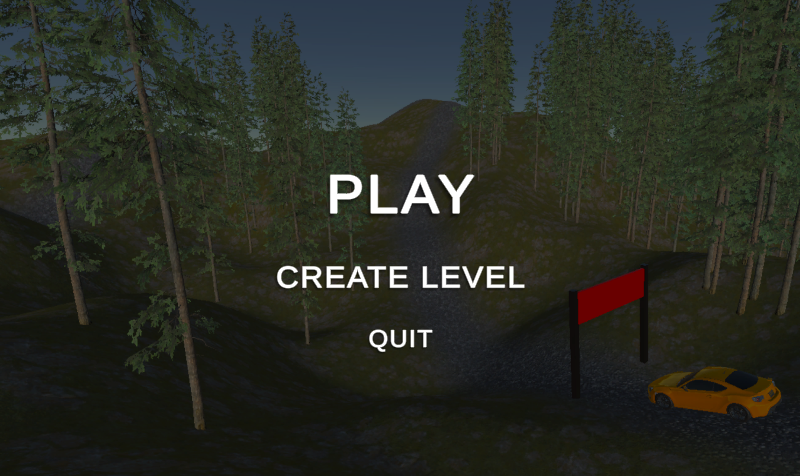
\includegraphics[width=.7\textwidth]{figures/game_instruction_start.png}
        \caption{Instruckja grania - ekran główny}
        \label{fig}
    \end{figure}
    Jeżeli użytkownik wybierze opcję gry, na kolejnym etapie zostanie poproszony o wybór poziomu oraz terenu. 
    Tereny utworzone przez użytkownika też pojawią się poniższym menu rozwijanym.
    \begin{figure}[H]
        \centering
        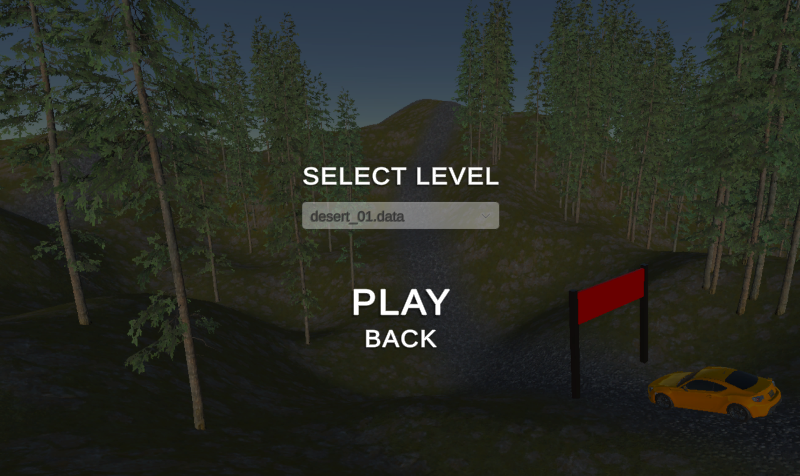
\includegraphics[width=.7\textwidth]{figures/game_instruction_choose_level.png}
        \caption{Instruckja grania - ekran główny}
        \label{fig}
    \end{figure}
    \clearpage
    Po włączeniu gry, wyścig rozpoczyna się od razu po dotknięciu ziemi. Do kontroli pojazdu należy używać strzałek na klawiaturze.
    \begin{figure}[H]
        \centering
        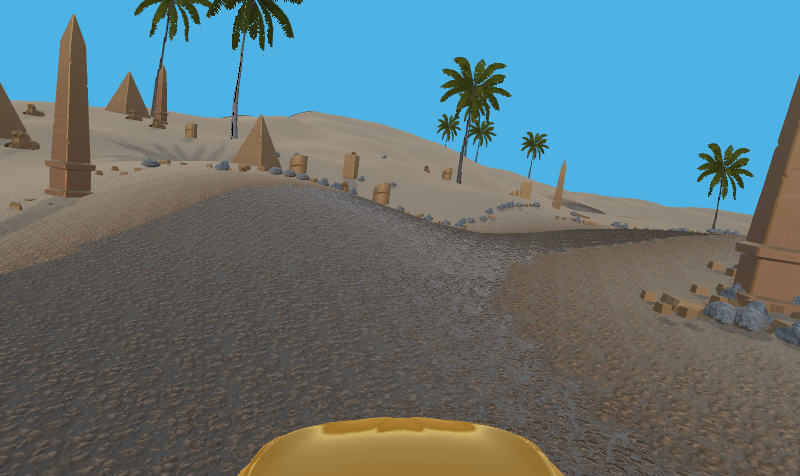
\includegraphics[width=.7\textwidth]{figures/game_instruction_play.png}
        \caption{Instruckja grania - ekran główny}
        \label{fig}
    \end{figure}
    Aby zatrzymać wyścig w trakcie, należy wcisnąć przycisk $Escape$ na klawiaturze. Czas w grze zostanie zatrzymany aż do wyłączenia widocznego menu.
    Można to osiągnąć wciskając ponownie $Escape$, lub wybierając opcję $Resume$ w menu. Dodatkowo użytkownik ma możliwość zakończyć grę i powrócić
    do głównego menu.
    \begin{figure}[H]
        \centering
        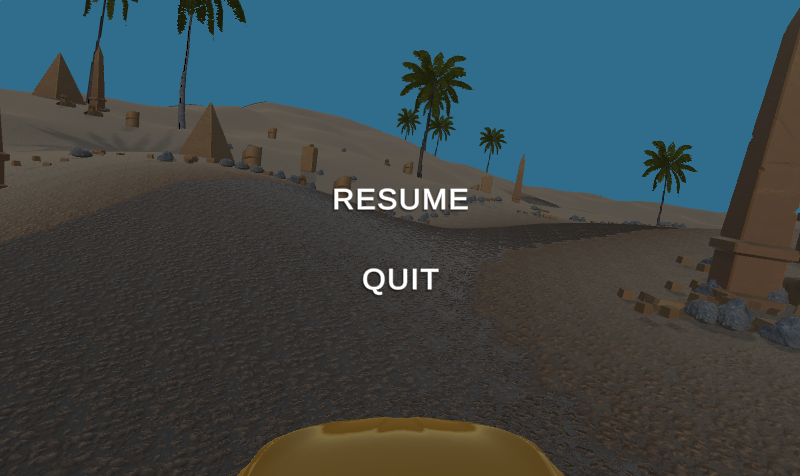
\includegraphics[width=.7\textwidth]{figures/game_instruction_pause.png}
        \caption{Instruckja grania - ekran główny}
        \label{fig}
    \end{figure}
    \clearpage
    Oprócz domyślnie zdefiniowanych poziomów i terenów, użytkownik ma możliwość wygenerować własną trasę, za pomocą kilku parametrów:
    \begin{itemize}
        \item Parametry $Complexity$ i $Seed$ definiują jak bardzo kręta będzie droga.
        \item Parametry $Details$, $Scale$ i $Offset$ pozwalają na określenie kształtu terenu.
        \item Parametr $Terrain$ określa szatę graficzną terenu.
    \end{itemize}
    Aby podejrzeć trasę z różnych stron można wykorzystać suwak $Preview Rotation$.\\
    Po ustawieniu wybranych parametrów, należy ustawić nazwę pliku w polu $Filename$. Pod taką nazwą pojawi się 
    wygenerowany teren podczas wyboru poziomu przed grą. Następnie należy kliknąć przycisk $Save$ aby zapisać teren.
    \begin{figure}[H]
        \centering
        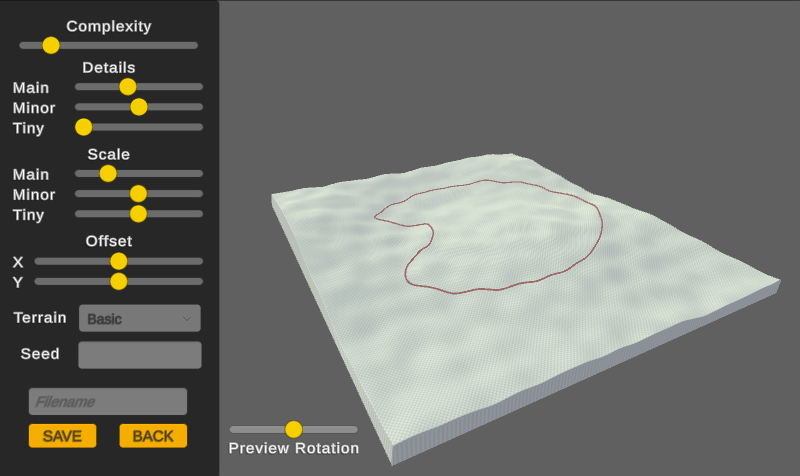
\includegraphics[width=.7\textwidth]{figures/game_instruction_create.png}
        \caption{Instruckja grania - ekran główny}
        \label{fig}
    \end{figure}
	\clearpage % \cleardoublepage 
	\chapter{Dokumentacja techniczna wygenerowana przez Doxygen (ENG)}
\thispagestyle{chapterBeginStyle}

\section{Namespace Index}
Here is a list of all documented namespaces with brief descriptions:
\begin{itemize}
\item[] \contentsline{section}{\mbox{\hyperlink{namespaceRacingGameBot}{RacingGameBot}} }{\pageref{namespaceRacingGameBot}}{}
\item[] \contentsline{section}{\mbox{\hyperlink{namespaceRacingGameBot_1_1Data}{RacingGameBot.Data}} }{\pageref{namespaceRacingGameBot_1_1Data}}{}
\item[] \contentsline{section}{\mbox{\hyperlink{namespaceRacingGameBot_1_1Editors}{RacingGameBot.Editors}} }{\pageref{namespaceRacingGameBot_1_1Editors}}{}
\item[] \contentsline{section}{\mbox{\hyperlink{namespaceRacingGameBot_1_1Menu}{RacingGameBot.Menu}} }{\pageref{namespaceRacingGameBot_1_1Menu}}{}
\item[] \contentsline{section}{\mbox{\hyperlink{namespaceRacingGameBot_1_1Play}{RacingGameBot.Play}} }{\pageref{namespaceRacingGameBot_1_1Play}}{}
\item[] \contentsline{section}{\mbox{\hyperlink{namespaceRacingGameBot_1_1Terrains}{RacingGameBot.Terrains}} }{\pageref{namespaceRacingGameBot_1_1Terrains}}{}
\item[] \contentsline{section}{\mbox{\hyperlink{namespaceRacingGameBot_1_1Tests}{RacingGameBot.Tests}} }{\pageref{namespaceRacingGameBot_1_1Tests}}{}
\item[] \contentsline{section}{\mbox{\hyperlink{namespaceRacingGameBot_1_1Utils}{RacingGameBot.Utils}} }{\pageref{namespaceRacingGameBot_1_1Utils}}{}
\end{itemize}
\clearpage
\section{Hierarchical Index}
This inheritance list is sorted roughly, but not completely, alphabetically:
\begin{itemize}
\item[] \contentsline{section}{\mbox{\hyperlink{classRacingGameBot_1_1Terrains_1_1Loop}{RacingGameBot.Terrains.Loop}}}{\pageref{classRacingGameBot_1_1Terrains_1_1Loop}}{}
\item[] \contentsline{section}{\mbox{\hyperlink{classRacingGameBot_1_1Terrains_1_1OrientedPoint}{RacingGameBot.Terrains.OrientedPoint}}}{\pageref{classRacingGameBot_1_1Terrains_1_1OrientedPoint}}{}
\end{itemize}
\textbf{Agent}
\begin{itemize}
\item[]  \contentsline{section}{\mbox{\hyperlink{classRacingGameBot_1_1Play_1_1CarAgent}{RacingGameBot.Play.CarAgent}}}{\pageref{classRacingGameBot_1_1Play_1_1CarAgent}}{}
\end{itemize}
\textbf{Editor}
\begin{itemize}
\item[]  \contentsline{section}{\mbox{\hyperlink{classRacingGameBot_1_1Editors_1_1TerrainGeneratorEditor}{RacingGameBot.Editors.TerrainGeneratorEditor}}}{\pageref{classRacingGameBot_1_1Editors_1_1TerrainGeneratorEditor}}{}
\item[]  \contentsline{section}{\mbox{\hyperlink{classRacingGameBot_1_1Editors_1_1TerrainLoaderEditor}{RacingGameBot.Editors.TerrainLoaderEditor}}}{\pageref{classRacingGameBot_1_1Editors_1_1TerrainLoaderEditor}}{}
\item[]  \contentsline{section}{\mbox{\hyperlink{classRacingGameBot_1_1Editors_1_1UpdatableDataEditor}{RacingGameBot.Editors.UpdatableDataEditor}}}{\pageref{classRacingGameBot_1_1Editors_1_1UpdatableDataEditor}}{}
\end{itemize}
\textbf{IPointerClickHandler}
\begin{itemize}
\item[]  \contentsline{section}{\mbox{\hyperlink{classRacingGameBot_1_1Menu_1_1ButtonActions}{RacingGameBot.Menu.ButtonActions}}}{\pageref{classRacingGameBot_1_1Menu_1_1ButtonActions}}{}
\end{itemize}
\textbf{IPointerEnterHandler}
\begin{itemize}
\item[]  \contentsline{section}{\mbox{\hyperlink{classRacingGameBot_1_1Menu_1_1ButtonActions}{RacingGameBot.Menu.ButtonActions}}}{\pageref{classRacingGameBot_1_1Menu_1_1ButtonActions}}{}
\end{itemize}
\textbf{IPointerExitHandler}
\begin{itemize}
\item[]  \contentsline{section}{\mbox{\hyperlink{classRacingGameBot_1_1Menu_1_1ButtonActions}{RacingGameBot.Menu.ButtonActions}}}{\pageref{classRacingGameBot_1_1Menu_1_1ButtonActions}}{}
\end{itemize}
\textbf{MonoBehaviour}
\begin{itemize}
\item[]  \contentsline{section}{\mbox{\hyperlink{classRacingGameBot_1_1Menu_1_1ButtonActions}{RacingGameBot.Menu.ButtonActions}}}{\pageref{classRacingGameBot_1_1Menu_1_1ButtonActions}}{}
\item[]  \contentsline{section}{\mbox{\hyperlink{classRacingGameBot_1_1Menu_1_1CreateLevelMenu}{RacingGameBot.Menu.CreateLevelMenu}}}{\pageref{classRacingGameBot_1_1Menu_1_1CreateLevelMenu}}{}
\item[]  \contentsline{section}{\mbox{\hyperlink{classRacingGameBot_1_1Menu_1_1EndMenu}{RacingGameBot.Menu.EndMenu}}}{\pageref{classRacingGameBot_1_1Menu_1_1EndMenu}}{}
\item[]  \contentsline{section}{\mbox{\hyperlink{classRacingGameBot_1_1Menu_1_1MainMenu}{RacingGameBot.Menu.MainMenu}}}{\pageref{classRacingGameBot_1_1Menu_1_1MainMenu}}{}
\item[]  \contentsline{section}{\mbox{\hyperlink{classRacingGameBot_1_1Menu_1_1PauseMenu}{RacingGameBot.Menu.PauseMenu}}}{\pageref{classRacingGameBot_1_1Menu_1_1PauseMenu}}{}
\item[]  \contentsline{section}{\mbox{\hyperlink{classRacingGameBot_1_1Play_1_1MultiTraining}{RacingGameBot.Play.MultiTraining}}}{\pageref{classRacingGameBot_1_1Play_1_1MultiTraining}}{}
\item[]  \contentsline{section}{\mbox{\hyperlink{classRacingGameBot_1_1Terrains_1_1TerrainGenerator}{RacingGameBot.Terrains.TerrainGenerator}}}{\pageref{classRacingGameBot_1_1Terrains_1_1TerrainGenerator}}{}
\item[]  \contentsline{section}{\mbox{\hyperlink{classRacingGameBot_1_1Terrains_1_1TerrainLoader}{RacingGameBot.Terrains.TerrainLoader}}}{\pageref{classRacingGameBot_1_1Terrains_1_1TerrainLoader}}{}
\item[]  \contentsline{section}{\mbox{\hyperlink{classRacingGameBot_1_1Tests_1_1BezierTests}{RacingGameBot.Tests.BezierTests}}}{\pageref{classRacingGameBot_1_1Tests_1_1BezierTests}}{}
\item[]  \contentsline{section}{\mbox{\hyperlink{classRacingGameBot_1_1Tests_1_1TextureTests}{RacingGameBot.Tests.TextureTests}}}{\pageref{classRacingGameBot_1_1Tests_1_1TextureTests}}{}
\item[]  \contentsline{section}{\mbox{\hyperlink{classRacingGameBot_1_1Utils_1_1Objects}{RacingGameBot.Utils.Objects}}}{\pageref{classRacingGameBot_1_1Utils_1_1Objects}}{}
\end{itemize}
\textbf{ScriptableObject}
\begin{itemize}
\item[]  \contentsline{section}{\mbox{\hyperlink{classRacingGameBot_1_1Data_1_1UpdatableData}{RacingGameBot.Data.UpdatableData}}}{\pageref{classRacingGameBot_1_1Data_1_1UpdatableData}}{}
\begin{itemize}
\item[]  \contentsline{section}{\mbox{\hyperlink{classRacingGameBot_1_1Data_1_1TerrainGenData}{RacingGameBot.Data.TerrainGenData}}}{\pageref{classRacingGameBot_1_1Data_1_1TerrainGenData}}{}
\end{itemize}
\end{itemize}

\clearpage
\section{Class Index}
Here are the classes, structs, unions and interfaces with brief descriptions:
\begin{itemize}
    \item[] \contentsline{section}{\mbox{\hyperlink{classRacingGameBot_1_1Data_1_1TerrainGenData}{RacingGameBot.Data.TerrainGenData}} }{\pageref{classRacingGameBot_1_1Data_1_1TerrainGenData}}{}
    \item[] \contentsline{section}{\mbox{\hyperlink{classRacingGameBot_1_1Data_1_1UpdatableData}{RacingGameBot.Data.UpdatableData}} }{\pageref{classRacingGameBot_1_1Data_1_1UpdatableData}}{}
    \item[] \contentsline{section}{\mbox{\hyperlink{classRacingGameBot_1_1Editors_1_1BuildScript}{RacingGameBot.Editors.BuildScript}} }{\pageref{classRacingGameBot_1_1Editors_1_1BuildScript}}{}
    \item[] \contentsline{section}{\mbox{\hyperlink{classRacingGameBot_1_1Editors_1_1TerrainGeneratorEditor}{RacingGameBot.Editors.TerrainGeneratorEditor}} }{\pageref{classRacingGameBot_1_1Editors_1_1TerrainGeneratorEditor}}{}
    \item[] \contentsline{section}{\mbox{\hyperlink{classRacingGameBot_1_1Editors_1_1TerrainLoaderEditor}{RacingGameBot.Editors.TerrainLoaderEditor}} }{\pageref{classRacingGameBot_1_1Editors_1_1TerrainLoaderEditor}}{}
    \item[] \contentsline{section}{\mbox{\hyperlink{classRacingGameBot_1_1Editors_1_1UpdatableDataEditor}{RacingGameBot.Editors.UpdatableDataEditor}} }{\pageref{classRacingGameBot_1_1Editors_1_1UpdatableDataEditor}}{}
    \item[] \contentsline{section}{\mbox{\hyperlink{classRacingGameBot_1_1Menu_1_1ButtonActions}{RacingGameBot.Menu.ButtonActions}} }{\pageref{classRacingGameBot_1_1Menu_1_1ButtonActions}}{}
    \item[] \contentsline{section}{\mbox{\hyperlink{classRacingGameBot_1_1Menu_1_1CreateLevelMenu}{RacingGameBot.Menu.CreateLevelMenu}} }{\pageref{classRacingGameBot_1_1Menu_1_1CreateLevelMenu}}{}
    \item[] \contentsline{section}{\mbox{\hyperlink{classRacingGameBot_1_1Menu_1_1EndMenu}{RacingGameBot.Menu.EndMenu}} }{\pageref{classRacingGameBot_1_1Menu_1_1EndMenu}}{}
    \item[] \contentsline{section}{\mbox{\hyperlink{classRacingGameBot_1_1Menu_1_1MainMenu}{RacingGameBot.Menu.MainMenu}} }{\pageref{classRacingGameBot_1_1Menu_1_1MainMenu}}{}
    \item[] \contentsline{section}{\mbox{\hyperlink{classRacingGameBot_1_1Menu_1_1PauseMenu}{RacingGameBot.Menu.PauseMenu}} }{\pageref{classRacingGameBot_1_1Menu_1_1PauseMenu}}{}
    \item[] \contentsline{section}{\mbox{\hyperlink{classRacingGameBot_1_1Play_1_1CarAgent}{RacingGameBot.Play.CarAgent}} }{\pageref{classRacingGameBot_1_1Play_1_1CarAgent}}{}
    \item[] \contentsline{section}{\mbox{\hyperlink{classRacingGameBot_1_1Play_1_1MultiTraining}{RacingGameBot.Play.MultiTraining}} }{\pageref{classRacingGameBot_1_1Play_1_1MultiTraining}}{}
    \item[] \contentsline{section}{\mbox{\hyperlink{classRacingGameBot_1_1Terrains_1_1Loop}{RacingGameBot.Terrains.Loop}} }{\pageref{classRacingGameBot_1_1Terrains_1_1Loop}}{}
    \item[] \contentsline{section}{\mbox{\hyperlink{classRacingGameBot_1_1Terrains_1_1OrientedPoint}{RacingGameBot.Terrains.OrientedPoint}} }{\pageref{classRacingGameBot_1_1Terrains_1_1OrientedPoint}}{}
    \item[] \contentsline{section}{\mbox{\hyperlink{classRacingGameBot_1_1Terrains_1_1TerrainGenerator}{RacingGameBot.Terrains.TerrainGenerator}} }{\pageref{classRacingGameBot_1_1Terrains_1_1TerrainGenerator}}{}
    \item[] \contentsline{section}{\mbox{\hyperlink{classRacingGameBot_1_1Terrains_1_1TerrainLoader}{RacingGameBot.Terrains.TerrainLoader}} }{\pageref{classRacingGameBot_1_1Terrains_1_1TerrainLoader}}{}
    \item[] \contentsline{section}{\mbox{\hyperlink{classRacingGameBot_1_1Tests_1_1BezierTests}{RacingGameBot.Tests.BezierTests}} }{\pageref{classRacingGameBot_1_1Tests_1_1BezierTests}}{}
    \item[] \contentsline{section}{\mbox{\hyperlink{classRacingGameBot_1_1Tests_1_1TextureTests}{RacingGameBot.Tests.TextureTests}} }{\pageref{classRacingGameBot_1_1Tests_1_1TextureTests}}{}
    \item[] \contentsline{section}{\mbox{\hyperlink{classRacingGameBot_1_1Utils_1_1Objects}{RacingGameBot.Utils.Objects}} }{\pageref{classRacingGameBot_1_1Utils_1_1Objects}}{}
\end{itemize}

\clearpage
\section{Namespace Documentation}

$\hypertarget{namespaceRacingGameBot_1_1Data}${}\subsection{RacingGameBot.Data Namespace Reference}
\label{namespaceRacingGameBot_1_1Data}\index{RacingGameBot.Data@{RacingGameBot.Data}}
\subsection*{Classes}
\begin{itemize}
\item[]  
class \mbox{\hyperlink{classRacingGameBot_1_1Data_1_1TerrainGenData}{TerrainGenData}}
\item[]  
class \mbox{\hyperlink{classRacingGameBot_1_1Data_1_1UpdatableData}{UpdatableData}}
\end{itemize}
\subsection*{Enumerations}
\begin{itemize}
\item[]  
\mbox{
$\hypertarget{namespaceRacingGameBot_1_1Data_a934234de471249eec8904fa48142acf8}$\label{namespaceRacingGameBot_1_1Data_a934234de471249eec8904fa48142acf8}} 
enum {\bfseries TerrainType} \{ {\bfseries Basic}, 
{\bfseries Forest}, 
{\bfseries Desert}, 
{\bfseries Mountains}
 \}
\end{itemize}


$\hypertarget{namespaceRacingGameBot_1_1Editors}${}\subsection{RacingGameBot.Editors Namespace Reference}
\label{namespaceRacingGameBot_1_1Editors}\index{RacingGameBot.Editors@{RacingGameBot.Editors}}
\subsection*{Classes}
\begin{itemize}
\item[]  
class \mbox{\hyperlink{classRacingGameBot_1_1Editors_1_1TerrainGeneratorEditor}{TerrainGeneratorEditor}}
\item[]  
class \mbox{\hyperlink{classRacingGameBot_1_1Editors_1_1TerrainLoaderEditor}{TerrainLoaderEditor}}
\item[]  
class \mbox{\hyperlink{classRacingGameBot_1_1Editors_1_1UpdatableDataEditor}{UpdatableDataEditor}}
\end{itemize}


$\hypertarget{namespaceRacingGameBot_1_1Menu}${}\subsection{RacingGameBot.Menu Namespace Reference}
\label{namespaceRacingGameBot_1_1Menu}\index{RacingGameBot.Menu@{RacingGameBot.Menu}}
\subsection*{Classes}
\begin{itemize}
\item[]  
class \mbox{\hyperlink{classRacingGameBot_1_1Menu_1_1ButtonActions}{ButtonActions}}
\item[]  
class \mbox{\hyperlink{classRacingGameBot_1_1Menu_1_1CreateLevelMenu}{CreateLevelMenu}}
\item[]  
class \mbox{\hyperlink{classRacingGameBot_1_1Menu_1_1EndMenu}{EndMenu}}
\item[]  
class \mbox{\hyperlink{classRacingGameBot_1_1Menu_1_1MainMenu}{MainMenu}}
\item[]  
class \mbox{\hyperlink{classRacingGameBot_1_1Menu_1_1PauseMenu}{PauseMenu}}
\end{itemize}


$\hypertarget{namespaceRacingGameBot_1_1Play}${}\subsection{RacingGameBot.Play Namespace Reference}
\label{namespaceRacingGameBot_1_1Play}\index{RacingGameBot.Play@{RacingGameBot.Play}}
\subsection*{Classes}
\begin{itemize}
\item[]  
class \mbox{\hyperlink{classRacingGameBot_1_1Play_1_1CarAgent}{CarAgent}}
\item[]  
class \mbox{\hyperlink{classRacingGameBot_1_1Play_1_1MultiTraining}{MultiTraining}}
\end{itemize}


$\hypertarget{namespaceRacingGameBot_1_1Terrains}${}\subsection{RacingGameBot.Terrains Namespace Reference}
\label{namespaceRacingGameBot_1_1Terrains}\index{RacingGameBot.Terrains@{RacingGameBot.Terrains}}
\subsection*{Classes}
\begin{itemize}
\item[]  
class \mbox{\hyperlink{classRacingGameBot_1_1Terrains_1_1Loop}{Loop}}
\item[]  
class \mbox{\hyperlink{classRacingGameBot_1_1Terrains_1_1OrientedPoint}{OrientedPoint}}
\item[]  
class \mbox{\hyperlink{classRacingGameBot_1_1Terrains_1_1TerrainGenerator}{TerrainGenerator}}
\item[]  
class \mbox{\hyperlink{classRacingGameBot_1_1Terrains_1_1TerrainLoader}{TerrainLoader}}
\end{itemize}


$\hypertarget{namespaceRacingGameBot_1_1Tests}${}\subsection{RacingGameBot.Tests Namespace Reference}
\label{namespaceRacingGameBot_1_1Tests}\index{RacingGameBot.Tests@{RacingGameBot.Tests}}
\subsection*{Classes}
\begin{itemize}
\item[]  
class \mbox{\hyperlink{classRacingGameBot_1_1Tests_1_1BezierTests}{BezierTests}}
\item[]  
class \mbox{\hyperlink{classRacingGameBot_1_1Tests_1_1TextureTests}{TextureTests}}
\end{itemize}
\subsection*{Enumerations}
\begin{itemize}
\item[]  
\mbox{
$\hypertarget{namespaceRacingGameBot_1_1Tests_a361ca3a4289ecb95145e3b102bf47e51}$\label{namespaceRacingGameBot_1_1Tests_a361ca3a4289ecb95145e3b102bf47e51}} 
enum {\bfseries MyTexture} \{
{\bfseries Grass1}, 
{\bfseries Grass2}, 
{\bfseries Grass3}, 
{\bfseries Road1}, 
\newline
{\phantom{.}\hspace{3.4cm}}
{\bfseries Road2}, 
{\bfseries Road3}, 
{\bfseries Road4}, 
{\bfseries Rocks1}, 
\newline
{\phantom{.}\hspace{3.4cm}}
{\bfseries Rocks2}, 
{\bfseries Rocks3}, 
{\bfseries Rocks4}, 
{\bfseries Sand1}, 
\newline
{\phantom{.}\hspace{3.4cm}}
{\bfseries Snow1}, 
{\bfseries Snow2}, 
{\bfseries Snow3}, 
{\bfseries Water1}
 \}
\end{itemize}


$\hypertarget{namespaceRacingGameBot_1_1Utils}${}\subsection{RacingGameBot.Utils Namespace Reference}
\label{namespaceRacingGameBot_1_1Utils}\index{RacingGameBot.Utils@{RacingGameBot.Utils}}
\subsection*{Classes}
\begin{itemize}
\item[]  
class \mbox{\hyperlink{classRacingGameBot_1_1Utils_1_1Bezier}{Bezier}}
\item[]  
class \mbox{\hyperlink{classRacingGameBot_1_1Utils_1_1Logging}{Logging}}
\item[]  
class \mbox{\hyperlink{classRacingGameBot_1_1Utils_1_1Objects}{Objects}}
\item[]  
class \mbox{\hyperlink{classRacingGameBot_1_1Utils_1_1Parser}{Parser}}
\item[]  
class {\bfseries Variables}
\end{itemize}

\clearpage
\section{Class Documentation}

$\hypertarget{classRacingGameBot_1_1Data_1_1TerrainGenData}${}
\subsection{RacingGameBot.Data.TerrainGenData Class Reference}
\label{classRacingGameBot_1_1Data_1_1TerrainGenData}
\index{RacingGameBot.Data.TerrainGenData@{RacingGameBot.Data.TerrainGenData}}

\begin{figure}[H]
    \minipage{.5\textwidth}
        \centering
        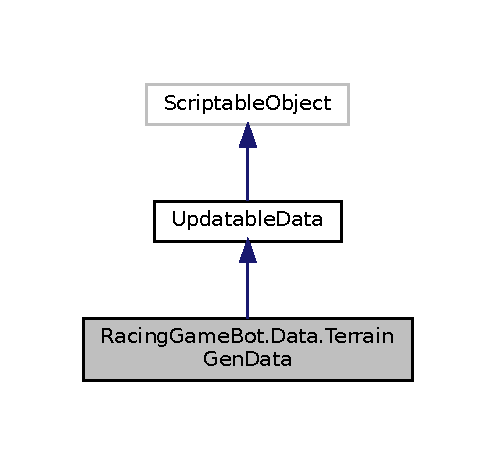
\includegraphics[height=6cm,width=\textwidth]{documentation/classRacingGameBot_1_1Data_1_1TerrainGenData__inherit__graph}
        \caption{Inheritance diagram for \\RacingGameBot.Data.TerrainGenData}
    \endminipage\hfill
    \minipage{.5\textwidth}
        \centering
        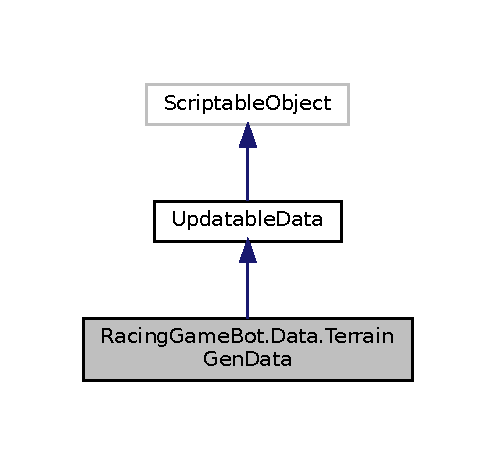
\includegraphics[height=6cm,width=\textwidth]{documentation/classRacingGameBot_1_1Data_1_1TerrainGenData__coll__graph}
        \caption{Collaboration diagram for \\RacingGameBot.Data.TerrainGenData}
    \endminipage
    \label{table}
\end{figure}

\subsection*{Public Attributes}
\begin{itemize}
\item[]  
\mbox{
$\hypertarget{classRacingGameBot_1_1Data_1_1TerrainGenData_a756c03f6cf15947fcf6104608322fd44}$\label{classRacingGameBot_1_1Data_1_1TerrainGenData_a756c03f6cf15947fcf6104608322fd44}} 
TerrainType {\bfseries terrainType} = TerrainType.Forest
\item[]  
\mbox{
$\hypertarget{classRacingGameBot_1_1Data_1_1TerrainGenData_ae8a9d9565a5145276535db6b349880c5}$\label{classRacingGameBot_1_1Data_1_1TerrainGenData_ae8a9d9565a5145276535db6b349880c5}} 
float {\bfseries roadLength} = 10000f
\item[]  
\mbox{
$\hypertarget{classRacingGameBot_1_1Data_1_1TerrainGenData_a0d7ec49edb64f38ca80630d55987ce42}$\label{classRacingGameBot_1_1Data_1_1TerrainGenData_a0d7ec49edb64f38ca80630d55987ce42}} 
float {\bfseries roadWidth} = 5f
\item[]  
\mbox{
$\hypertarget{classRacingGameBot_1_1Data_1_1TerrainGenData_af4f8b5e832ad69ffe900492cc57b3a68}$\label{classRacingGameBot_1_1Data_1_1TerrainGenData_af4f8b5e832ad69ffe900492cc57b3a68}} 
float {\bfseries paddingPercent} = 0.2f
\item[]  
\mbox{
$\hypertarget{classRacingGameBot_1_1Data_1_1TerrainGenData_ad6f588fd83b9df587bae88513110df71}$\label{classRacingGameBot_1_1Data_1_1TerrainGenData_ad6f588fd83b9df587bae88513110df71}} 
int {\bfseries numberOfSegments} = 4
\item[]  
\mbox{
$\hypertarget{classRacingGameBot_1_1Data_1_1TerrainGenData_a80906b30111603c08b0c4a583bdd0d17}$\label{classRacingGameBot_1_1Data_1_1TerrainGenData_a80906b30111603c08b0c4a583bdd0d17}} 
int {\bfseries numberOfCheckpoints} = 40
\item[]  
\mbox{
$\hypertarget{classRacingGameBot_1_1Data_1_1TerrainGenData_a9394749be05237f5546badbf3df0f230}$\label{classRacingGameBot_1_1Data_1_1TerrainGenData_a9394749be05237f5546badbf3df0f230}} 
float {\bfseries terrainDetailsMain} = 0.3f
\item[]  
\mbox{
$\hypertarget{classRacingGameBot_1_1Data_1_1TerrainGenData_af2434d9fa14aac9cc12885c03105466c}$\label{classRacingGameBot_1_1Data_1_1TerrainGenData_af2434d9fa14aac9cc12885c03105466c}} 
float {\bfseries terrainDetailsMinor} = 0.05f
\item[]  
\mbox{
$\hypertarget{classRacingGameBot_1_1Data_1_1TerrainGenData_aec6d065171e74d43974832f4c21e1a49}$\label{classRacingGameBot_1_1Data_1_1TerrainGenData_aec6d065171e74d43974832f4c21e1a49}} 
float {\bfseries terrainDetailsTiny} = 0f
\item[]  
\mbox{
$\hypertarget{classRacingGameBot_1_1Data_1_1TerrainGenData_adebaf3347c878710539b9d8894ef0380}$\label{classRacingGameBot_1_1Data_1_1TerrainGenData_adebaf3347c878710539b9d8894ef0380}} 
float {\bfseries terrainScaleMain} = 1.5f
\item[]  
\mbox{
$\hypertarget{classRacingGameBot_1_1Data_1_1TerrainGenData_a5575916e45db5976fb2588d2a577bd78}$\label{classRacingGameBot_1_1Data_1_1TerrainGenData_a5575916e45db5976fb2588d2a577bd78}} 
float {\bfseries terrainScaleMinor} = 5f
\item[]  
\mbox{
$\hypertarget{classRacingGameBot_1_1Data_1_1TerrainGenData_a4071a6fe5204dd23d27da5b06f12081a}$\label{classRacingGameBot_1_1Data_1_1TerrainGenData_a4071a6fe5204dd23d27da5b06f12081a}} 
float {\bfseries terrainScaleTiny} = 5f
\item[]  
\mbox{
$\hypertarget{classRacingGameBot_1_1Data_1_1TerrainGenData_acd96f308654123433c51f888cbdbfc4f}$\label{classRacingGameBot_1_1Data_1_1TerrainGenData_acd96f308654123433c51f888cbdbfc4f}} 
float {\bfseries offsetX} = 0f
\item[]  
\mbox{
$\hypertarget{classRacingGameBot_1_1Data_1_1TerrainGenData_a5795a026e2bb2d1151da1174ba0feb4b}$\label{classRacingGameBot_1_1Data_1_1TerrainGenData_a5795a026e2bb2d1151da1174ba0feb4b}} 
float {\bfseries offsetY} = 0f
\end{itemize}


$\hypertarget{classRacingGameBot_1_1Data_1_1UpdatableData}${}
\subsection{RacingGameBot.Data.UpdatableData Class Reference}
\label{classRacingGameBot_1_1Data_1_1UpdatableData}
\index{RacingGameBot.Data.UpdatableData@{RacingGameBot.Data.UpdatableData}}

\begin{figure}[H]
    \minipage{.5\textwidth}
        \centering
        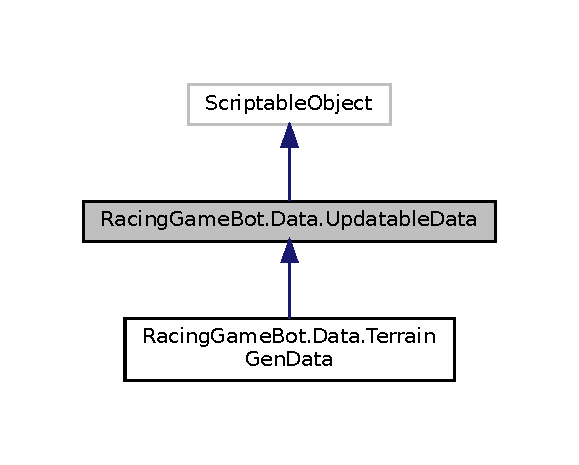
\includegraphics[height=6cm,width=\textwidth, width=\textwidth]{documentation/classRacingGameBot_1_1Data_1_1UpdatableData__inherit__graph}
        \caption{Inheritance diagram for \\RacingGameBot.Data.UpdatableData}
    \endminipage\hfill
    \minipage{.5\textwidth}
        \centering
        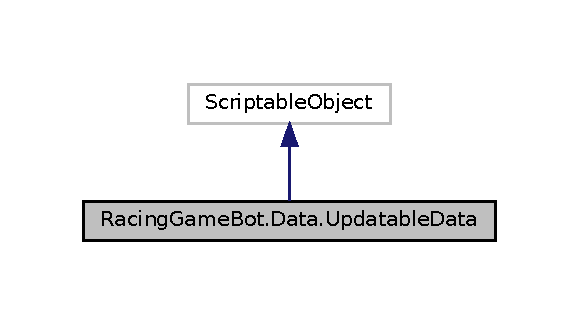
\includegraphics[height=6cm,width=\textwidth, width=\textwidth]{documentation/classRacingGameBot_1_1Data_1_1UpdatableData__coll__graph}
        \caption{Collaboration diagram for \\RacingGameBot.Data.UpdatableData}
    \endminipage
    \label{table}
\end{figure}

\subsection*{Public Member Functions}
\begin{itemize}
\item[]  
\mbox{
$\hypertarget{classRacingGameBot_1_1Data_1_1UpdatableData_add26db43395c4547d0c8fd76e94e51c3}$\label{classRacingGameBot_1_1Data_1_1UpdatableData_add26db43395c4547d0c8fd76e94e51c3}} 
void {\bfseries NotifyOfUpdatedValues} ()
\end{itemize}
\subsection*{Public Attributes}
\begin{itemize}
\item[]  
\mbox{
$\hypertarget{classRacingGameBot_1_1Data_1_1UpdatableData_a572bfb45eefe6f2e643e505918af2bf7}$\label{classRacingGameBot_1_1Data_1_1UpdatableData_a572bfb45eefe6f2e643e505918af2bf7}} 
bool {\bfseries autoUpdate} = true
\end{itemize}
\subsection*{Protected Member Functions}
\begin{itemize}
\item[]  
\mbox{
$\hypertarget{classRacingGameBot_1_1Data_1_1UpdatableData_adc8402ca40e13d163906b7d3d1916b91}$\label{classRacingGameBot_1_1Data_1_1UpdatableData_adc8402ca40e13d163906b7d3d1916b91}} 
virtual void {\bfseries OnValidate} ()
\end{itemize}


$\hypertarget{classRacingGameBot_1_1Editors_1_1TerrainGeneratorEditor}${}
\subsection{RacingGameBot.Editors.TerrainGeneratorEditor Class Reference}
\label{classRacingGameBot_1_1Editors_1_1TerrainGeneratorEditor}
\index{RacingGameBot.Editors.TerrainGeneratorEditor@{RacingGameBot.Editors.TerrainGeneratorEditor}}

\begin{figure}[H]
    \minipage{.5\textwidth}
        \centering
        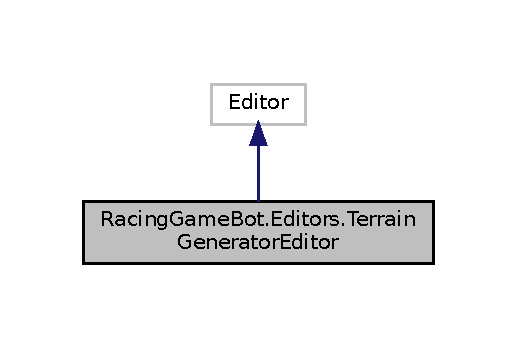
\includegraphics[height=6cm,width=\textwidth]{documentation/classRacingGameBot_1_1Editors_1_1TerrainGeneratorEditor__inherit__graph}
        \caption{Inheritance diagram for \\RacingGameBot.Editors.TerrainGeneratorEditor}
    \endminipage\hfill
    \minipage{.5\textwidth}
        \centering
        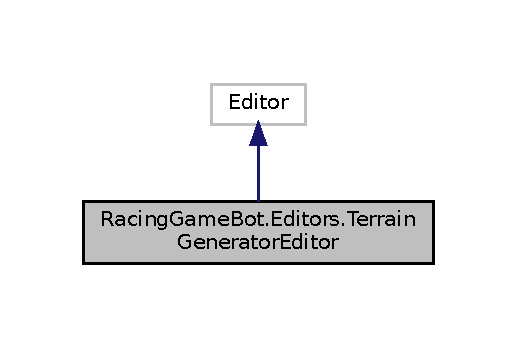
\includegraphics[height=6cm,width=\textwidth]{documentation/classRacingGameBot_1_1Editors_1_1TerrainGeneratorEditor__coll__graph}
        \caption{Collaboration diagram for \\RacingGameBot.Editors.TerrainGeneratorEditor}
    \endminipage
    \label{table}
\end{figure}

\subsection*{Public Member Functions}
\begin{itemize}
\item[]  
\mbox{
$\hypertarget{classRacingGameBot_1_1Editors_1_1TerrainGeneratorEditor_a01ab9749ab3a63bf274fe07cdd347aa3}$\label{classRacingGameBot_1_1Editors_1_1TerrainGeneratorEditor_a01ab9749ab3a63bf274fe07cdd347aa3}} 
override void {\bfseries OnInspectorGUI} ()
\end{itemize}





$\hypertarget{classRacingGameBot_1_1Editors_1_1TerrainLoaderEditor}${}
\subsection{RacingGameBot.Editors.TerrainLoaderEditor Class Reference}
\label{classRacingGameBot_1_1Editors_1_1TerrainLoaderEditor}
\index{RacingGameBot.Editors.TerrainLoaderEditor@{RacingGameBot.Editors.TerrainLoaderEditor}}

\begin{figure}[H]
    \minipage{.5\textwidth}
        \centering
        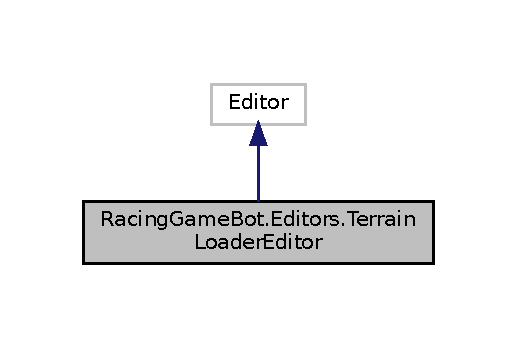
\includegraphics[height=6cm,width=\textwidth]{documentation/classRacingGameBot_1_1Editors_1_1TerrainLoaderEditor__inherit__graph}
        \caption{Inheritance diagram for \\RacingGameBot.Editors.TerrainLoaderEditor}
    \endminipage\hfill
    \minipage{.5\textwidth}
        \centering
        \includegraphics[height=6cm,width=\textwidth]{documentation/classRacingGameBot_1_1Editors_1_1TerrainLoaderEditor__coll__graph}
        \caption{Collaboration diagram for \\RacingGameBot.Editors.TerrainLoaderEditor}
    \endminipage
    \label{table}
\end{figure}

\subsection*{Public Member Functions}
\begin{itemize}
\item[]  
\mbox{
$\hypertarget{classRacingGameBot_1_1Editors_1_1TerrainLoaderEditor_a8203eeab1e9301fbe15e633e7d197cf3}$\label{classRacingGameBot_1_1Editors_1_1TerrainLoaderEditor_a8203eeab1e9301fbe15e633e7d197cf3}} 
override void {\bfseries OnInspectorGUI} ()
\end{itemize}





$\hypertarget{classRacingGameBot_1_1Editors_1_1UpdatableDataEditor}${}
\subsection{RacingGameBot.Editors.UpdatableDataEditor Class Reference}
\label{classRacingGameBot_1_1Editors_1_1UpdatableDataEditor}
\index{RacingGameBot.Editors.UpdatableDataEditor@{RacingGameBot.Editors.UpdatableDataEditor}}

\begin{figure}[H]
    \minipage{.5\textwidth}
        \centering
        \includegraphics[height=6cm,width=\textwidth]{documentation/classRacingGameBot_1_1Editors_1_1UpdatableDataEditor__inherit__graph}
        \caption{Inheritance diagram for \\RacingGameBot.Editors.UpdatableDataEditor}
    \endminipage\hfill
    \minipage{.5\textwidth}
        \centering
        \includegraphics[height=6cm,width=\textwidth]{documentation/classRacingGameBot_1_1Editors_1_1UpdatableDataEditor__coll__graph}
        \caption{Collaboration diagram for \\RacingGameBot.Editors.UpdatableDataEditor}
    \endminipage
    \label{table}
\end{figure}

\subsection*{Public Member Functions}
\begin{itemize}
\item[]  
\mbox{
$\hypertarget{classRacingGameBot_1_1Editors_1_1UpdatableDataEditor_a0cff1d28a00268c21ca1cc2a577e9cbb}$\label{classRacingGameBot_1_1Editors_1_1UpdatableDataEditor_a0cff1d28a00268c21ca1cc2a577e9cbb}} 
override void {\bfseries OnInspectorGUI} ()
\end{itemize}





$\hypertarget{classRacingGameBot_1_1Menu_1_1ButtonActions}${}
\subsection{RacingGameBot.Menu.ButtonActions Class Reference}
\label{classRacingGameBot_1_1Menu_1_1ButtonActions}
\index{RacingGameBot.Menu.ButtonActions@{RacingGameBot.Menu.ButtonActions}}

\begin{figure}[H]
    \minipage{.5\textwidth}
        \centering
        \includegraphics[height=4cm,width=\textwidth]{documentation/classRacingGameBot_1_1Menu_1_1ButtonActions__inherit__graph}
        \caption{Inheritance diagram for \\RacingGameBot.Menu.ButtonActions}
    \endminipage\hfill
    \minipage{.5\textwidth}
        \centering
        \includegraphics[height=4cm,width=\textwidth]{documentation/classRacingGameBot_1_1Menu_1_1ButtonActions__coll__graph}
        \caption{Collaboration diagram for \\RacingGameBot.Menu.ButtonActions}
    \endminipage
    \label{table}
\end{figure}

\subsection*{Public Member Functions}
\begin{itemize}
\item[]  
void \mbox{\hyperlink{classRacingGameBot_1_1Menu_1_1ButtonActions_a72e5acacfd7928bf963a45fcc8f9437a}{OnPointerEnter}} (PointerEventData eventData)
\begin{itemize}\small\item[] \em Change text size and color on hover enter \end{itemize}\item[]  
void \mbox{\hyperlink{classRacingGameBot_1_1Menu_1_1ButtonActions_ae3a9640f3ce7550ed2ad918c676483d2}{OnPointerExit}} (PointerEventData eventData)
\begin{itemize}\small\item[] \em Change text size and color on hover exit \end{itemize}\item[]  
void \mbox{\hyperlink{classRacingGameBot_1_1Menu_1_1ButtonActions_a160f0a10845ee3feab339248835de0d4}{OnPointerClick}} (PointerEventData eventData)
\begin{itemize}\small\item[] \em Change text size and color on click \end{itemize}\end{itemize}


\subsection{Member Function Documentation}
\mbox{
$\hypertarget{classRacingGameBot_1_1Menu_1_1ButtonActions_a160f0a10845ee3feab339248835de0d4}$
\label{classRacingGameBot_1_1Menu_1_1ButtonActions_a160f0a10845ee3feab339248835de0d4}} 
\index{RacingGameBot.Menu.ButtonActions@{RacingGameBot.Menu.ButtonActions}!OnPointerClick@{OnPointerClick}}
\index{OnPointerClick@{OnPointerClick}!RacingGameBot.Menu.ButtonActions@{RacingGameBot.Menu.ButtonActions}}
\subsubsection{\texorpdfstring{OnPointerClick()}{OnPointerClick()}}
{\footnotesize\ttfamily void RacingGameBot.Menu.ButtonActions.OnPointerClick (\begin{itemize}
    \item[] [{PointerEventData}]{ eventData }
\end{itemize}\hspace{0.5cm})}\\
Change text size and color on click \\
\begin{tabular}{|c|c|}
\hline
{\em eventData} & Click event data\\
\hline
\end{tabular}
\mbox{
$\hypertarget{classRacingGameBot_1_1Menu_1_1ButtonActions_a72e5acacfd7928bf963a45fcc8f9437a}$\label{classRacingGameBot_1_1Menu_1_1ButtonActions_a72e5acacfd7928bf963a45fcc8f9437a}} 
\index{RacingGameBot.Menu.ButtonActions@{RacingGameBot.Menu.ButtonActions}!OnPointerEnter@{OnPointerEnter}}
\index{OnPointerEnter@{OnPointerEnter}!RacingGameBot.Menu.ButtonActions@{RacingGameBot.Menu.ButtonActions}}
\subsubsection{\texorpdfstring{OnPointerEnter()}{OnPointerEnter()}}
{\footnotesize\ttfamily void RacingGameBot.Menu.ButtonActions.OnPointerEnter (\begin{itemize}
    \item[] [{PointerEventData}]{ eventData }
\end{itemize}\hspace{0.5cm})}\\
Change text size and color on hover enter \\
\begin{tabular}{|c|c|}
\hline
{\em eventData} & Hover event data\\
\hline
\end{tabular}
\mbox{
$\hypertarget{classRacingGameBot_1_1Menu_1_1ButtonActions_ae3a9640f3ce7550ed2ad918c676483d2}$\label{classRacingGameBot_1_1Menu_1_1ButtonActions_ae3a9640f3ce7550ed2ad918c676483d2}} 
\index{RacingGameBot.Menu.ButtonActions@{RacingGameBot.Menu.ButtonActions}!OnPointerExit@{OnPointerExit}}
\index{OnPointerExit@{OnPointerExit}!RacingGameBot.Menu.ButtonActions@{RacingGameBot.Menu.ButtonActions}}
\subsubsection{\texorpdfstring{OnPointerExit()}{OnPointerExit()}}
{\footnotesize\ttfamily void RacingGameBot.Menu.ButtonActions.OnPointerExit (\begin{itemize}
    \item[] [{PointerEventData}]{ eventData }
\end{itemize}\hspace{0.5cm})}\\
Change text size and color on hover exit \\
\begin{tabular}{|c|c|}
\hline
{\em eventData} & Hover event data\\
\hline
\end{tabular}


$\hypertarget{classRacingGameBot_1_1Menu_1_1CreateLevelMenu}${}
\subsection{RacingGameBot.Menu.CreateLevelMenu Class Reference}
\label{classRacingGameBot_1_1Menu_1_1CreateLevelMenu}
\index{RacingGameBot.Menu.CreateLevelMenu@{RacingGameBot.Menu.CreateLevelMenu}}

\begin{figure}[H]
    \minipage{.5\textwidth}
        \centering
        \includegraphics[height=6cm,width=\textwidth]{documentation/classRacingGameBot_1_1Menu_1_1CreateLevelMenu__inherit__graph}
        \caption{Inheritance diagram for \\RacingGameBot.Menu.CreateLevelMenu}
    \endminipage\hfill
    \minipage{.5\textwidth}
        \centering
        \includegraphics[height=6cm,width=\textwidth]{documentation/classRacingGameBot_1_1Menu_1_1CreateLevelMenu__coll__graph}
        \caption{Collaboration diagram for \\RacingGameBot.Menu.CreateLevelMenu}
    \endminipage
    \label{table}
\end{figure}

\subsection*{Public Member Functions}
\begin{itemize}
\item[]  
void \mbox{\hyperlink{classRacingGameBot_1_1Menu_1_1CreateLevelMenu_aeefe9a031d628b82297173dc5b856d80}{Rotate}} (float angle)
\begin{itemize}\small\item[] \em Rotate terrain preview \end{itemize}\item[]  
void \mbox{\hyperlink{classRacingGameBot_1_1Menu_1_1CreateLevelMenu_a56958398e057b987a5b491e976dd7c1b}{MenuOptionChangeComplexity}} (float value)
\begin{itemize}\small\item[] \em Change road complexity \end{itemize}\item[]  
\mbox{
$\hypertarget{classRacingGameBot_1_1Menu_1_1CreateLevelMenu_af94b87cbec7c65368ee41780fcb59a7a}$\label{classRacingGameBot_1_1Menu_1_1CreateLevelMenu_af94b87cbec7c65368ee41780fcb59a7a}} 
void {\bfseries MenuOptionChangeDetailsMain} (float value)
\item[] 
\mbox{
$\hypertarget{classRacingGameBot_1_1Menu_1_1CreateLevelMenu_af7e8362303e9e90522c3eae03fa45562}$\label{classRacingGameBot_1_1Menu_1_1CreateLevelMenu_af7e8362303e9e90522c3eae03fa45562}} 
void {\bfseries MenuOptionChangeDetailsMinor} (float value)
\item[]  
\mbox{
$\hypertarget{classRacingGameBot_1_1Menu_1_1CreateLevelMenu_aced7101c37b14b9a6040eb1651813dd7}$\label{classRacingGameBot_1_1Menu_1_1CreateLevelMenu_aced7101c37b14b9a6040eb1651813dd7}} 
void {\bfseries MenuOptionChangeDetailsTiny} (float value)
\item[]  
\mbox{
$\hypertarget{classRacingGameBot_1_1Menu_1_1CreateLevelMenu_aeac42aba612248afb1715f2c71b0175f}$\label{classRacingGameBot_1_1Menu_1_1CreateLevelMenu_aeac42aba612248afb1715f2c71b0175f}} 
void {\bfseries MenuOptionChangeScaleMain} (float value)
\item[]  
\mbox{
$\hypertarget{classRacingGameBot_1_1Menu_1_1CreateLevelMenu_a4cf94039bb8c539cb946fbefb1f36191}$\label{classRacingGameBot_1_1Menu_1_1CreateLevelMenu_a4cf94039bb8c539cb946fbefb1f36191}} 
void {\bfseries MenuOptionChangeScaleMinor} (float value)
\item[]  
\mbox{
$\hypertarget{classRacingGameBot_1_1Menu_1_1CreateLevelMenu_a50f8259400bb35c77b2eca2a7a2d27cb}$\label{classRacingGameBot_1_1Menu_1_1CreateLevelMenu_a50f8259400bb35c77b2eca2a7a2d27cb}} 
void {\bfseries MenuOptionChangeScaleTiny} (float value)
\item[]  
\mbox{
$\hypertarget{classRacingGameBot_1_1Menu_1_1CreateLevelMenu_adf931acd8c93fc199e1633e6ba0a0080}$\label{classRacingGameBot_1_1Menu_1_1CreateLevelMenu_adf931acd8c93fc199e1633e6ba0a0080}} 
void {\bfseries MenuOptionChangeOffsetX} (float value)
\item[]  
\mbox{
$\hypertarget{classRacingGameBot_1_1Menu_1_1CreateLevelMenu_a7fe9b58f6bf2afbf1099c2bbf92264c8}$\label{classRacingGameBot_1_1Menu_1_1CreateLevelMenu_a7fe9b58f6bf2afbf1099c2bbf92264c8}} 
void {\bfseries MenuOptionChangeOffsetY} (float value)
\item[]  
\mbox{
$\hypertarget{classRacingGameBot_1_1Menu_1_1CreateLevelMenu_a4120fc2a18e72a7c2b40f2e080937330}$\label{classRacingGameBot_1_1Menu_1_1CreateLevelMenu_a4120fc2a18e72a7c2b40f2e080937330}} 
void {\bfseries MenuOptionChangeTerrainType} (int value)
\item[]  
void \mbox{\hyperlink{classRacingGameBot_1_1Menu_1_1CreateLevelMenu_a50db0eada1894b0c509391b704a2edec}{MenuOptionChangeSeed}} (string value)
\begin{itemize}\small\item[] \em Change road generation seed \end{itemize}\item[]  
void \mbox{\hyperlink{classRacingGameBot_1_1Menu_1_1CreateLevelMenu_a36af14418f24a46562b0186806bb2c0c}{MenuOptionSetFilename}} (string value)
\begin{itemize}\small\item[] \em Change save filename \end{itemize}\item[]  
void \mbox{\hyperlink{classRacingGameBot_1_1Menu_1_1CreateLevelMenu_a5a69e99b1d0fe6ec5b81fc4a673b8518}{Save}} ()
\begin{itemize}\small\item[] \em Save generated terrain \end{itemize}\item[]  
void \mbox{\hyperlink{classRacingGameBot_1_1Menu_1_1CreateLevelMenu_acdbfd1423fefe7db51b1336925bcef73}{SaveCallbackUpdateTime}} (int percentage)
\begin{itemize}\small\item[] \em Update saving progress \end{itemize}\item[]  
void \mbox{\hyperlink{classRacingGameBot_1_1Menu_1_1CreateLevelMenu_ab6bc390673f31e29acad052cb56b5309}{SaveCallbackEnd}} ()
\begin{itemize}\small\item[] \em Open main menu after finished saving \end{itemize}\end{itemize}
\subsection*{Public Attributes}
\begin{itemize}
\item[]  
\mbox{
$\hypertarget{classRacingGameBot_1_1Menu_1_1CreateLevelMenu_ab380e34ce50acdc815cd46df68148f14}$\label{classRacingGameBot_1_1Menu_1_1CreateLevelMenu_ab380e34ce50acdc815cd46df68148f14}} 
GameObject {\bfseries terrainGO}
\item[]  
\mbox{
$\hypertarget{classRacingGameBot_1_1Menu_1_1CreateLevelMenu_af7c2b164b9949c1bacfa4338b8dc1b92}$\label{classRacingGameBot_1_1Menu_1_1CreateLevelMenu_af7c2b164b9949c1bacfa4338b8dc1b92}} 
GameObject {\bfseries cameraGO}
\item[]  
\mbox{
$\hypertarget{classRacingGameBot_1_1Menu_1_1CreateLevelMenu_a76800a79c3e4957332074a2af02ae6ed}$\label{classRacingGameBot_1_1Menu_1_1CreateLevelMenu_a76800a79c3e4957332074a2af02ae6ed}} 
GameObject {\bfseries panelGO}
\item[]  
\mbox{
$\hypertarget{classRacingGameBot_1_1Menu_1_1CreateLevelMenu_adfa5d9ef26e758c6c879217776b621e8}$\label{classRacingGameBot_1_1Menu_1_1CreateLevelMenu_adfa5d9ef26e758c6c879217776b621e8}} 
GameObject {\bfseries loadingGO}
\end{itemize}


\subsection{Member Function Documentation}
\mbox{
$\hypertarget{classRacingGameBot_1_1Menu_1_1CreateLevelMenu_a56958398e057b987a5b491e976dd7c1b}$\label{classRacingGameBot_1_1Menu_1_1CreateLevelMenu_a56958398e057b987a5b491e976dd7c1b}} 
\index{RacingGameBot.Menu.CreateLevelMenu@{RacingGameBot.Menu.CreateLevelMenu}!MenuOptionChangeComplexity@{MenuOptionChangeComplexity}}
\index{MenuOptionChangeComplexity@{MenuOptionChangeComplexity}!RacingGameBot.Menu.CreateLevelMenu@{RacingGameBot.Menu.CreateLevelMenu}}
\subsubsection{\texorpdfstring{MenuOptionChangeComplexity()}{MenuOptionChangeComplexity()}}
{\footnotesize\ttfamily void RacingGameBot.Menu.CreateLevelMenu.MenuOptionChangeComplexity (\begin{itemize}
    \item[] [{float}]{ value }
\end{itemize}\hspace{0.5cm})}\\
Change road complexity \\
\begin{tabular}{|c|c|}
\hline
{\em value} & Complexity\\
\hline
\end{tabular}
\mbox{
$\hypertarget{classRacingGameBot_1_1Menu_1_1CreateLevelMenu_a50db0eada1894b0c509391b704a2edec}$\label{classRacingGameBot_1_1Menu_1_1CreateLevelMenu_a50db0eada1894b0c509391b704a2edec}} 
\index{RacingGameBot.Menu.CreateLevelMenu@{RacingGameBot.Menu.CreateLevelMenu}!MenuOptionChangeSeed@{MenuOptionChangeSeed}}
\index{MenuOptionChangeSeed@{MenuOptionChangeSeed}!RacingGameBot.Menu.CreateLevelMenu@{RacingGameBot.Menu.CreateLevelMenu}}
\subsubsection{\texorpdfstring{MenuOptionChangeSeed()}{MenuOptionChangeSeed()}}
{\footnotesize\ttfamily void RacingGameBot.Menu.CreateLevelMenu.MenuOptionChangeSeed (\begin{itemize}
    \item[] [{string}]{ value }
\end{itemize}\hspace{0.5cm})}\\
Change road generation seed \\
\begin{tabular}{|c|c|}
\hline
{\em value} & Seed\\
\hline
\end{tabular}
\mbox{
$\hypertarget{classRacingGameBot_1_1Menu_1_1CreateLevelMenu_a36af14418f24a46562b0186806bb2c0c}$\label{classRacingGameBot_1_1Menu_1_1CreateLevelMenu_a36af14418f24a46562b0186806bb2c0c}} 
\index{RacingGameBot.Menu.CreateLevelMenu@{RacingGameBot.Menu.CreateLevelMenu}!MenuOptionSetFilename@{MenuOptionSetFilename}}
\index{MenuOptionSetFilename@{MenuOptionSetFilename}!RacingGameBot.Menu.CreateLevelMenu@{RacingGameBot.Menu.CreateLevelMenu}}
\subsubsection{\texorpdfstring{MenuOptionSetFilename()}{MenuOptionSetFilename()}}
{\footnotesize\ttfamily void RacingGameBot.Menu.CreateLevelMenu.MenuOptionSetFilename (\begin{itemize}
    \item[] [{string}]{ value }
\end{itemize}\hspace{0.5cm})}\\
Change save filename \\
\begin{tabular}{|c|c|}
\hline
{\em value} & Complexity\\
\hline
\end{tabular}
\mbox{
$\hypertarget{classRacingGameBot_1_1Menu_1_1CreateLevelMenu_aeefe9a031d628b82297173dc5b856d80}$\label{classRacingGameBot_1_1Menu_1_1CreateLevelMenu_aeefe9a031d628b82297173dc5b856d80}} 
\index{RacingGameBot.Menu.CreateLevelMenu@{RacingGameBot.Menu.CreateLevelMenu}!Rotate@{Rotate}}
\index{Rotate@{Rotate}!RacingGameBot.Menu.CreateLevelMenu@{RacingGameBot.Menu.CreateLevelMenu}}
\subsubsection{\texorpdfstring{Rotate()}{Rotate()}}
{\footnotesize\ttfamily void RacingGameBot.Menu.CreateLevelMenu.Rotate (\begin{itemize}
    \item[] [{string}]{ value }
\end{itemize}\hspace{0.5cm})}\\
Rotate terrain preview \\
\begin{tabular}{|c|c|}
\hline
{\em angle} & Angle\\
\hline
\end{tabular}
\mbox{
$\hypertarget{classRacingGameBot_1_1Menu_1_1CreateLevelMenu_a5a69e99b1d0fe6ec5b81fc4a673b8518}$\label{classRacingGameBot_1_1Menu_1_1CreateLevelMenu_a5a69e99b1d0fe6ec5b81fc4a673b8518}} 
\index{RacingGameBot.Menu.CreateLevelMenu@{RacingGameBot.Menu.CreateLevelMenu}!Save@{Save}}
\index{Save@{Save}!RacingGameBot.Menu.CreateLevelMenu@{RacingGameBot.Menu.CreateLevelMenu}}
\subsubsection{\texorpdfstring{Save()}{Save()}}
{\footnotesize\ttfamily void RacingGameBot.Menu.CreateLevelMenu.Save (\begin{itemize}
    \item[] [{string}]{ value }
\end{itemize}\hspace{0.5cm})}\\
Save generated terrain \\
\mbox{
$\hypertarget{classRacingGameBot_1_1Menu_1_1CreateLevelMenu_ab6bc390673f31e29acad052cb56b5309}$\label{classRacingGameBot_1_1Menu_1_1CreateLevelMenu_ab6bc390673f31e29acad052cb56b5309}} 
\index{RacingGameBot.Menu.CreateLevelMenu@{RacingGameBot.Menu.CreateLevelMenu}!SaveCallbackEnd@{SaveCallbackEnd}}
\index{SaveCallbackEnd@{SaveCallbackEnd}!RacingGameBot.Menu.CreateLevelMenu@{RacingGameBot.Menu.CreateLevelMenu}}
\subsubsection{\texorpdfstring{SaveCallbackEnd()}{SaveCallbackEnd()}}
{\footnotesize\ttfamily void RacingGameBot.Menu.CreateLevelMenu.SaveCallbackEnd (\begin{itemize}
    \item[] [{string}]{ value }
\end{itemize}\hspace{0.5cm})}\\
Open main menu after finished saving \\
\mbox{
$\hypertarget{classRacingGameBot_1_1Menu_1_1CreateLevelMenu_acdbfd1423fefe7db51b1336925bcef73}$\label{classRacingGameBot_1_1Menu_1_1CreateLevelMenu_acdbfd1423fefe7db51b1336925bcef73}} 
\index{RacingGameBot.Menu.CreateLevelMenu@{RacingGameBot.Menu.CreateLevelMenu}!SaveCallbackUpdateTime@{SaveCallbackUpdateTime}}
\index{SaveCallbackUpdateTime@{SaveCallbackUpdateTime}!RacingGameBot.Menu.CreateLevelMenu@{RacingGameBot.Menu.CreateLevelMenu}}
\subsubsection{\texorpdfstring{SaveCallbackUpdateTime()}{SaveCallbackUpdateTime()}}
{\footnotesize\ttfamily void RacingGameBot.Menu.CreateLevelMenu.SaveCallbackUpdateTime (\begin{itemize}
    \item[] [{string}]{ value }
\end{itemize}\hspace{0.5cm})}\\
Update saving progress


$\hypertarget{classRacingGameBot_1_1Menu_1_1EndMenu}${}
\subsection{RacingGameBot.Menu.EndMenu Class Reference}
\label{classRacingGameBot_1_1Menu_1_1EndMenu}
\index{RacingGameBot.Menu.EndMenu@{RacingGameBot.Menu.EndMenu}}

\begin{figure}[H]
    \minipage{.5\textwidth}
        \centering
        \includegraphics[height=6cm,width=\textwidth]{documentation/classRacingGameBot_1_1Menu_1_1EndMenu__inherit__graph}
        \caption{Inheritance diagram for \\RacingGameBot.Menu.EndMenu}
    \endminipage\hfill
    \minipage{.5\textwidth}
        \centering
        \includegraphics[height=6cm,width=\textwidth]{documentation/classRacingGameBot_1_1Menu_1_1EndMenu__coll__graph}
        \caption{Collaboration diagram for \\RacingGameBot.Menu.EndMenu}
    \endminipage
    \label{table}
\end{figure}

\subsection*{Public Member Functions}
\begin{itemize}
\item[]  
void \mbox{\hyperlink{classRacingGameBot_1_1Menu_1_1EndMenu_a202ecc8422c9e2ed6b1973fc9eb45181}{Show}} (bool won)
\begin{itemize}\small\item[] \em Show menu at the end of race \end{itemize}\item[]  
void \mbox{\hyperlink{classRacingGameBot_1_1Menu_1_1EndMenu_aa518c1103af22934bfa9551e3213587a}{QuitGame}} ()
\begin{itemize}\small\item[] \em Quit game and return to main menu \end{itemize}\end{itemize}
\subsection*{Public Attributes}
\begin{itemize}
\item[]  
\mbox{
$\hypertarget{classRacingGameBot_1_1Menu_1_1EndMenu_a59b5ef628b88fcbd2e0abe49f93b40ba}$\label{classRacingGameBot_1_1Menu_1_1EndMenu_a59b5ef628b88fcbd2e0abe49f93b40ba}} 
GameObject {\bfseries endMenu}
\item[]  
\mbox{
$\hypertarget{classRacingGameBot_1_1Menu_1_1EndMenu_aff767a041cdd74ea15117ad426ee8890}$\label{classRacingGameBot_1_1Menu_1_1EndMenu_aff767a041cdd74ea15117ad426ee8890}} 
GameObject {\bfseries winningText}
\end{itemize}


\subsection{Member Function Documentation}
\mbox{
$\hypertarget{classRacingGameBot_1_1Menu_1_1EndMenu_aa518c1103af22934bfa9551e3213587a}$\label{classRacingGameBot_1_1Menu_1_1EndMenu_aa518c1103af22934bfa9551e3213587a}} 
\index{RacingGameBot.Menu.EndMenu@{RacingGameBot.Menu.EndMenu}!QuitGame@{QuitGame}}
\index{QuitGame@{QuitGame}!RacingGameBot.Menu.EndMenu@{RacingGameBot.Menu.EndMenu}}
\subsubsection{\texorpdfstring{QuitGame()}{QuitGame()}}
{\footnotesize\ttfamily void RacingGameBot.Menu.EndMenu.QuitGame ()}\\
Quit game and return to main menu \\
\mbox{
$\hypertarget{classRacingGameBot_1_1Menu_1_1EndMenu_a202ecc8422c9e2ed6b1973fc9eb45181}$\label{classRacingGameBot_1_1Menu_1_1EndMenu_a202ecc8422c9e2ed6b1973fc9eb45181}} 
\index{RacingGameBot.Menu.EndMenu@{RacingGameBot.Menu.EndMenu}!Show@{Show}}
\index{Show@{Show}!RacingGameBot.Menu.EndMenu@{RacingGameBot.Menu.EndMenu}}
\subsubsection{\texorpdfstring{Show()}{Show()}}
{\footnotesize\ttfamily void RacingGameBot.Menu.EndMenu.Show (\begin{itemize}
    \item[] [{bool}]{ won }
\end{itemize}\hspace{0.5cm})}\\
Show menu at the end of race \\
\begin{tabular}{|c|c|}
\hline
{\em won} & Whether user won or lost\\
\hline
\end{tabular}


$\hypertarget{classRacingGameBot_1_1Menu_1_1MainMenu}${}
\subsection{RacingGameBot.Menu.MainMenu Class Reference}
\label{classRacingGameBot_1_1Menu_1_1MainMenu}
\index{RacingGameBot.Menu.MainMenu@{RacingGameBot.Menu.MainMenu}}

\begin{figure}[H]
    \minipage{.5\textwidth}
        \centering
        \includegraphics[height=6cm,width=\textwidth]{documentation/classRacingGameBot_1_1Menu_1_1MainMenu__inherit__graph}
        \caption{Inheritance diagram for \\RacingGameBot.Menu.MainMenu}
    \endminipage\hfill
    \minipage{.5\textwidth}
        \centering
        \includegraphics[height=6cm,width=\textwidth]{documentation/classRacingGameBot_1_1Menu_1_1MainMenu__coll__graph}
        \caption{Collaboration diagram for \\RacingGameBot.Menu.MainMenu}
    \endminipage
    \label{table}
\end{figure}

\subsection*{Public Member Functions}
\begin{itemize}
\item[]  
void \mbox{\hyperlink{classRacingGameBot_1_1Menu_1_1MainMenu_a887833310427a90ded2cce76fd4c327e}{MenuOptionPlayGame}} ()
\begin{itemize}\small\item[] \em Open play screen \end{itemize}\item[]  
void \mbox{\hyperlink{classRacingGameBot_1_1Menu_1_1MainMenu_a171838b0e899d4ff7f69f17f9d8493f0}{MenuOptionCreateLevel}} ()
\begin{itemize}\small\item[] \em Open level creation screen \end{itemize}\item[]  
void \mbox{\hyperlink{classRacingGameBot_1_1Menu_1_1MainMenu_a10fc2fc042f1cafd3c7d41e9674fd306}{MenuOptionQuitGame}} ()
\begin{itemize}\small\item[] \em Quit game \end{itemize}\item[]  
void \mbox{\hyperlink{classRacingGameBot_1_1Menu_1_1MainMenu_ad6661998082e12ba4147b71fcf20a238}{MenuOptionMoveToPlayMenu}} ()
\begin{itemize}\small\item[] \em Open play level choosing screen \end{itemize}\item[]  
void \mbox{\hyperlink{classRacingGameBot_1_1Menu_1_1MainMenu_a2fa3418e23de32ab9aa22a1214e32c48}{MenuOptionMoveToMainMenu}} ()
\begin{itemize}\small\item[] \em Get back from level choosing screen to main screen \end{itemize}\item[]  
void \mbox{\hyperlink{classRacingGameBot_1_1Menu_1_1MainMenu_aa4a7ca98389901423bd5759b4f59b1bb}{MenuOptionChooseFilename}} (int file)
\begin{itemize}\small\item[] \em Select level name \end{itemize}\end{itemize}
\subsection*{Public Attributes}
\begin{itemize}
\item[]  
\mbox{
$\hypertarget{classRacingGameBot_1_1Menu_1_1MainMenu_a4993e410c5f90bea25f2c1c019f0d6a3}$\label{classRacingGameBot_1_1Menu_1_1MainMenu_a4993e410c5f90bea25f2c1c019f0d6a3}} 
string {\bfseries filename}
\item[]  
\mbox{
$\hypertarget{classRacingGameBot_1_1Menu_1_1MainMenu_a9135ce6bc7750f6e718f8a3d9f51ddff}$\label{classRacingGameBot_1_1Menu_1_1MainMenu_a9135ce6bc7750f6e718f8a3d9f51ddff}} 
List$<$ TMPro.TMP\_Dropdown.OptionData $>$ {\bfseries options}
\item[]  
\mbox{
$\hypertarget{classRacingGameBot_1_1Menu_1_1MainMenu_a4145c06e9ebac85a2826aa7d8e928569}$\label{classRacingGameBot_1_1Menu_1_1MainMenu_a4145c06e9ebac85a2826aa7d8e928569}} 
GameObject {\bfseries mainMenu}
\item[]  
\mbox{
$\hypertarget{classRacingGameBot_1_1Menu_1_1MainMenu_a033a89e6d19004fb291b8e526707d2b6}$\label{classRacingGameBot_1_1Menu_1_1MainMenu_a033a89e6d19004fb291b8e526707d2b6}} 
GameObject {\bfseries playMenu}
\end{itemize}


\subsection{Member Function Documentation}
\mbox{
$\hypertarget{classRacingGameBot_1_1Menu_1_1MainMenu_aa4a7ca98389901423bd5759b4f59b1bb}$\label{classRacingGameBot_1_1Menu_1_1MainMenu_aa4a7ca98389901423bd5759b4f59b1bb}} 
\index{RacingGameBot.Menu.MainMenu@{RacingGameBot.Menu.MainMenu}!MenuOptionChooseFilename@{MenuOptionChooseFilename}}
\index{MenuOptionChooseFilename@{MenuOptionChooseFilename}!RacingGameBot.Menu.MainMenu@{RacingGameBot.Menu.MainMenu}}
\subsubsection{\texorpdfstring{MenuOptionChooseFilename()}{MenuOptionChooseFilename()}}
{\footnotesize\ttfamily void RacingGameBot.Menu.MainMenu.MenuOptionChooseFilename (\begin{itemize}
    \item[] [{int}]{ file }
\end{itemize}\hspace{0.6cm})}\\
Select level name \\
\begin{tabular}{|c|c|}
\hline
{\em file} & Number of file on the list\\
\hline
\end{tabular}
\mbox{
$\hypertarget{classRacingGameBot_1_1Menu_1_1MainMenu_a171838b0e899d4ff7f69f17f9d8493f0}$\label{classRacingGameBot_1_1Menu_1_1MainMenu_a171838b0e899d4ff7f69f17f9d8493f0}} 
\index{RacingGameBot.Menu.MainMenu@{RacingGameBot.Menu.MainMenu}!MenuOptionCreateLevel@{MenuOptionCreateLevel}}
\index{MenuOptionCreateLevel@{MenuOptionCreateLevel}!RacingGameBot.Menu.MainMenu@{RacingGameBot.Menu.MainMenu}}
\subsubsection{\texorpdfstring{MenuOptionCreateLevel()}{MenuOptionCreateLevel()}}
{\footnotesize\ttfamily void RacingGameBot.Menu.MainMenu.MenuOptionCreateLevel ()}\\
Open level creation screen \\
\mbox{
$\hypertarget{classRacingGameBot_1_1Menu_1_1MainMenu_a2fa3418e23de32ab9aa22a1214e32c48}$\label{classRacingGameBot_1_1Menu_1_1MainMenu_a2fa3418e23de32ab9aa22a1214e32c48}} 
\index{RacingGameBot.Menu.MainMenu@{RacingGameBot.Menu.MainMenu}!MenuOptionMoveToMainMenu@{MenuOptionMoveToMainMenu}}
\index{MenuOptionMoveToMainMenu@{MenuOptionMoveToMainMenu}!RacingGameBot.Menu.MainMenu@{RacingGameBot.Menu.MainMenu}}
\subsubsection{\texorpdfstring{MenuOptionMoveToMainMenu()}{MenuOptionMoveToMainMenu()}}
{\footnotesize\ttfamily void RacingGameBot.Menu.MainMenu.MenuOptionMoveToMainMenu ()}\\
Get back from level choosing screen to main screen \\
\mbox{
$\hypertarget{classRacingGameBot_1_1Menu_1_1MainMenu_ad6661998082e12ba4147b71fcf20a238}$\label{classRacingGameBot_1_1Menu_1_1MainMenu_ad6661998082e12ba4147b71fcf20a238}} 
\index{RacingGameBot.Menu.MainMenu@{RacingGameBot.Menu.MainMenu}!MenuOptionMoveToPlayMenu@{MenuOptionMoveToPlayMenu}}
\index{MenuOptionMoveToPlayMenu@{MenuOptionMoveToPlayMenu}!RacingGameBot.Menu.MainMenu@{RacingGameBot.Menu.MainMenu}}
\subsubsection{\texorpdfstring{MenuOptionMoveToPlayMenu()}{MenuOptionMoveToPlayMenu()}}
{\footnotesize\ttfamily void RacingGameBot.Menu.MainMenu.MenuOptionMoveToPlayMenu ()}\\
Open play level choosing screen \\
\mbox{
$\hypertarget{classRacingGameBot_1_1Menu_1_1MainMenu_a887833310427a90ded2cce76fd4c327e}$\label{classRacingGameBot_1_1Menu_1_1MainMenu_a887833310427a90ded2cce76fd4c327e}} 
\index{RacingGameBot.Menu.MainMenu@{RacingGameBot.Menu.MainMenu}!MenuOptionPlayGame@{MenuOptionPlayGame}}
\index{MenuOptionPlayGame@{MenuOptionPlayGame}!RacingGameBot.Menu.MainMenu@{RacingGameBot.Menu.MainMenu}}
\subsubsection{\texorpdfstring{MenuOptionPlayGame()}{MenuOptionPlayGame()}}
{\footnotesize\ttfamily void RacingGameBot.Menu.MainMenu.MenuOptionPlayGame ()}\\
Open play screen \\
\mbox{
$\hypertarget{classRacingGameBot_1_1Menu_1_1MainMenu_a10fc2fc042f1cafd3c7d41e9674fd306}$\label{classRacingGameBot_1_1Menu_1_1MainMenu_a10fc2fc042f1cafd3c7d41e9674fd306}} 
\index{RacingGameBot.Menu.MainMenu@{RacingGameBot.Menu.MainMenu}!MenuOptionQuitGame@{MenuOptionQuitGame}}
\index{MenuOptionQuitGame@{MenuOptionQuitGame}!RacingGameBot.Menu.MainMenu@{RacingGameBot.Menu.MainMenu}}
\subsubsection{\texorpdfstring{MenuOptionQuitGame()}{MenuOptionQuitGame()}}
{\footnotesize\ttfamily void RacingGameBot.Menu.MainMenu.MenuOptionQuitGame ()}\\
Quit game 


$\hypertarget{classRacingGameBot_1_1Menu_1_1PauseMenu}${}
\subsection{RacingGameBot.Menu.PauseMenu Class Reference}
\label{classRacingGameBot_1_1Menu_1_1PauseMenu}
\index{RacingGameBot.Menu.PauseMenu@{RacingGameBot.Menu.PauseMenu}}

\begin{figure}[H]
    \minipage{.5\textwidth}
        \centering
        \includegraphics[height=6cm,width=\textwidth]{documentation/classRacingGameBot_1_1Menu_1_1PauseMenu__inherit__graph}
        \caption{Inheritance diagram for \\RacingGameBot.Menu.PauseMenu}
    \endminipage\hfill
    \minipage{.5\textwidth}
        \centering
        \includegraphics[height=6cm,width=\textwidth]{documentation/classRacingGameBot_1_1Menu_1_1PauseMenu__coll__graph}
        \caption{Collaboration diagram for \\RacingGameBot.Menu.PauseMenu}
    \endminipage
    \label{table}
\end{figure}

\subsection*{Public Member Functions}
\begin{itemize}
\item[]  
void \mbox{\hyperlink{classRacingGameBot_1_1Menu_1_1PauseMenu_a1f4b7cb24f38d90ffdc1779185760fa3}{ResumeGame}} ()
\begin{itemize}\small\item[] \em Hide menu and resume game \end{itemize}\item[]  
void \mbox{\hyperlink{classRacingGameBot_1_1Menu_1_1PauseMenu_a9baa2bdb94290ec0fd43bfeb85d5bfb6}{PauseGame}} ()
\begin{itemize}\small\item[] \em Show menu and pause game \end{itemize}\item[]  
void \mbox{\hyperlink{classRacingGameBot_1_1Menu_1_1PauseMenu_ae1a0062b73b17ad50d728e5e34830511}{QuitGame}} ()
\begin{itemize}\small\item[] \em Quit game and open main menu \end{itemize}\end{itemize}
\subsection*{Public Attributes}
\begin{itemize}
\item[]  
\mbox{
$\hypertarget{classRacingGameBot_1_1Menu_1_1PauseMenu_a5ac6c06667b933dad3ddd034a12dfbfb}$\label{classRacingGameBot_1_1Menu_1_1PauseMenu_a5ac6c06667b933dad3ddd034a12dfbfb}} 
GameObject {\bfseries pauseMenu}
\end{itemize}
\subsection*{Static Public Attributes}
\begin{itemize}
\item[]  
\mbox{
$\hypertarget{classRacingGameBot_1_1Menu_1_1PauseMenu_a8c9afdf925d9eb44027c4015e68656df}$\label{classRacingGameBot_1_1Menu_1_1PauseMenu_a8c9afdf925d9eb44027c4015e68656df}} 
static bool {\bfseries gameIsPaused} = false
\end{itemize}


\subsection{Member Function Documentation}
\mbox{
$\hypertarget{classRacingGameBot_1_1Menu_1_1PauseMenu_a9baa2bdb94290ec0fd43bfeb85d5bfb6}$\label{classRacingGameBot_1_1Menu_1_1PauseMenu_a9baa2bdb94290ec0fd43bfeb85d5bfb6}} 
\index{RacingGameBot.Menu.PauseMenu@{RacingGameBot.Menu.PauseMenu}!PauseGame@{PauseGame}}
\index{PauseGame@{PauseGame}!RacingGameBot.Menu.PauseMenu@{RacingGameBot.Menu.PauseMenu}}
\subsubsection{\texorpdfstring{PauseGame()}{PauseGame()}}
{\footnotesize\ttfamily void RacingGameBot.Menu.PauseMenu.PauseGame ()}\\
Show menu and pause game \\
\mbox{
$\hypertarget{classRacingGameBot_1_1Menu_1_1PauseMenu_ae1a0062b73b17ad50d728e5e34830511}$\label{classRacingGameBot_1_1Menu_1_1PauseMenu_ae1a0062b73b17ad50d728e5e34830511}} 
\index{RacingGameBot.Menu.PauseMenu@{RacingGameBot.Menu.PauseMenu}!QuitGame@{QuitGame}}
\index{QuitGame@{QuitGame}!RacingGameBot.Menu.PauseMenu@{RacingGameBot.Menu.PauseMenu}}
\subsubsection{\texorpdfstring{QuitGame()}{QuitGame()}}
{\footnotesize\ttfamily void RacingGameBot.Menu.PauseMenu.QuitGame ()}\\
Quit game and open main menu \\
\mbox{
$\hypertarget{classRacingGameBot_1_1Menu_1_1PauseMenu_a1f4b7cb24f38d90ffdc1779185760fa3}$\label{classRacingGameBot_1_1Menu_1_1PauseMenu_a1f4b7cb24f38d90ffdc1779185760fa3}} 
\index{RacingGameBot.Menu.PauseMenu@{RacingGameBot.Menu.PauseMenu}!ResumeGame@{ResumeGame}}
\index{ResumeGame@{ResumeGame}!RacingGameBot.Menu.PauseMenu@{RacingGameBot.Menu.PauseMenu}}
\subsubsection{\texorpdfstring{ResumeGame()}{ResumeGame()}}
{\footnotesize\ttfamily void RacingGameBot.Menu.PauseMenu.ResumeGame ()}\\
Hide menu and resume game 


$\hypertarget{classRacingGameBot_1_1Play_1_1CarAgent}${}
\subsection{RacingGameBot.Play.CarAgent Class Reference}
\label{classRacingGameBot_1_1Play_1_1CarAgent}
\index{RacingGameBot.Play.CarAgent@{RacingGameBot.Play.CarAgent}}

\begin{figure}[H]
    \minipage{.5\textwidth}
        \centering
        \includegraphics[height=6cm,width=\textwidth]{documentation/classRacingGameBot_1_1Play_1_1CarAgent__inherit__graph}
        \caption{Inheritance diagram for \\RacingGameBot.Play.CarAgent}
    \endminipage\hfill
    \minipage{.5\textwidth}
        \centering
        \includegraphics[height=6cm,width=\textwidth]{documentation/classRacingGameBot_1_1Play_1_1CarAgent__coll__graph}
        \caption{Collaboration diagram for \\RacingGameBot.Play.CarAgent}
    \endminipage
    \label{table}
\end{figure}

\subsection*{Public Member Functions}
\begin{itemize}
\item[]  
override void \mbox{\hyperlink{classRacingGameBot_1_1Play_1_1CarAgent_a1a88dadc71f190f4bd9000fc92fcf534}{OnEpisodeBegin}} ()
\begin{itemize}\small\item[] \em Set car starting position in first episode, reset it at the beginning of each episode \end{itemize}\item[]  
override void \mbox{\hyperlink{classRacingGameBot_1_1Play_1_1CarAgent_a200700254aa02bef33edf50af522be7a}{CollectObservations}} (VectorSensor sensor)
\begin{itemize}\small\item[] \em Collect observation data from environment \end{itemize}\item[]  
override void \mbox{\hyperlink{classRacingGameBot_1_1Play_1_1CarAgent_ab0dddeeecc837714465d40e5ede7d507}{OnActionReceived}} (ActionBuffers actions)
\begin{itemize}\small\item[] \em Move car based on inference results and assign rewards \end{itemize}\item[]  
void \mbox{\hyperlink{classRacingGameBot_1_1Play_1_1CarAgent_a60320fcbd4ee7a3a4a636d6c5f51a9fa}{OnTriggerEnter}} (Collider other)
\begin{itemize}\small\item[] \em Handle car collisions with environment objects, like other cars, checkpoints, finish, etc. \end{itemize}\item[]  
override void \mbox{\hyperlink{classRacingGameBot_1_1Play_1_1CarAgent_a5fe0055071343b94e121f2ca9094c164}{Heuristic}} (in ActionBuffers actionsOut)
\begin{itemize}\small\item[] \em Read user inputs for manual steering \end{itemize}\end{itemize}
\subsection*{Public Attributes}
\begin{itemize}
\item[]  
\mbox{
$\hypertarget{classRacingGameBot_1_1Play_1_1CarAgent_affd085f2b1f07fdbebbd91679ef1eadb}$
    \label{classRacingGameBot_1_1Play_1_1CarAgent_affd085f2b1f07fdbebbd91679ef1eadb}
}
bool {showGizmos} = false
\item[]  
\mbox{
$\hypertarget{classRacingGameBot_1_1Play_1_1CarAgent_a13d1204dbc73500078ef58644f6311a8}$\label{classRacingGameBot_1_1Play_1_1CarAgent_a13d1204dbc73500078ef58644f6311a8}} 
bool {\bfseries playMode} = false
\end{itemize}


\subsection{Member Function Documentation}
\mbox{
$\hypertarget{classRacingGameBot_1_1Play_1_1CarAgent_a200700254aa02bef33edf50af522be7a}$\label{classRacingGameBot_1_1Play_1_1CarAgent_a200700254aa02bef33edf50af522be7a}} 
\index{RacingGameBot.Play.CarAgent@{RacingGameBot.Play.CarAgent}!CollectObservations@{CollectObservations}}
\index{CollectObservations@{CollectObservations}!RacingGameBot.Play.CarAgent@{RacingGameBot.Play.CarAgent}}
\subsubsection{\texorpdfstring{CollectObservations()}{CollectObservations()}}
{\footnotesize\ttfamily override void RacingGameBot.Play.CarAgent.CollectObservations (\begin{itemize}
    \item[] [{VectorSensor}]{ sensor }
\end{itemize}\hspace{0.5cm})}\\
Collect observation data from environment: \\
$\cdot$ distance to road center\\
$\cdot$ current input axis positions for forward and sideways movement\\
$\cdot$ slope of terrain\\
$\cdot$ velocity\\
\begin{tabular}{|c|c|}
\hline
{\em sensor} & Car sensor\\
\hline
\end{tabular}
\mbox{
$\hypertarget{classRacingGameBot_1_1Play_1_1CarAgent_a5fe0055071343b94e121f2ca9094c164}$\label{classRacingGameBot_1_1Play_1_1CarAgent_a5fe0055071343b94e121f2ca9094c164}} 
\index{RacingGameBot.Play.CarAgent@{RacingGameBot.Play.CarAgent}!Heuristic@{Heuristic}}
\index{Heuristic@{Heuristic}!RacingGameBot.Play.CarAgent@{RacingGameBot.Play.CarAgent}}
\subsubsection{\texorpdfstring{Heuristic()}{Heuristic()}}
{\footnotesize\ttfamily override void RacingGameBot.Play.CarAgent.Heuristic (\begin{itemize}
    \item[] [{in ActionBuffers}]{ actionsOut }
\end{itemize}\hspace{0.5cm})}\\
Read user inputs for manual steering \\
\begin{tabular}{|c|c|}
\hline
{\em actionsOut} & Car actions\\
\hline
\end{tabular}
\mbox{
$\hypertarget{classRacingGameBot_1_1Play_1_1CarAgent_ab0dddeeecc837714465d40e5ede7d507}$\label{classRacingGameBot_1_1Play_1_1CarAgent_ab0dddeeecc837714465d40e5ede7d507}} 
\index{RacingGameBot.Play.CarAgent@{RacingGameBot.Play.CarAgent}!OnActionReceived@{OnActionReceived}}
\index{OnActionReceived@{OnActionReceived}!RacingGameBot.Play.CarAgent@{RacingGameBot.Play.CarAgent}}
\subsubsection{\texorpdfstring{OnActionReceived()}{OnActionReceived()}}
{\footnotesize\ttfamily override void RacingGameBot.Play.CarAgent.OnActionReceived (\begin{itemize}
    \item[] [{ActionBuffers}]{ actions }
\end{itemize}\hspace{0.5cm})}\\
Move car based on inference results and assign rewards \\
\begin{tabular}{|c|c|}
\hline
{\em actions} & Received actions\\
\hline
\end{tabular}
\mbox{
$\hypertarget{classRacingGameBot_1_1Play_1_1CarAgent_a1a88dadc71f190f4bd9000fc92fcf534}$\label{classRacingGameBot_1_1Play_1_1CarAgent_a1a88dadc71f190f4bd9000fc92fcf534}} 
\index{RacingGameBot.Play.CarAgent@{RacingGameBot.Play.CarAgent}!OnEpisodeBegin@{OnEpisodeBegin}}
\index{OnEpisodeBegin@{OnEpisodeBegin}!RacingGameBot.Play.CarAgent@{RacingGameBot.Play.CarAgent}}
\subsubsection{\texorpdfstring{OnEpisodeBegin()}{OnEpisodeBegin()}}
{\footnotesize\ttfamily override void RacingGameBot.Play.CarAgent.OnEpisodeBegin()}\\
Set car starting position in first episode, reset it at the beginning of each episode \\
\mbox{
$\hypertarget{classRacingGameBot_1_1Play_1_1CarAgent_a60320fcbd4ee7a3a4a636d6c5f51a9fa}$\label{classRacingGameBot_1_1Play_1_1CarAgent_a60320fcbd4ee7a3a4a636d6c5f51a9fa}} 
\index{RacingGameBot.Play.CarAgent@{RacingGameBot.Play.CarAgent}!OnTriggerEnter@{OnTriggerEnter}}
\index{OnTriggerEnter@{OnTriggerEnter}!RacingGameBot.Play.CarAgent@{RacingGameBot.Play.CarAgent}}
\subsubsection{\texorpdfstring{OnTriggerEnter()}{OnTriggerEnter()}}
{\footnotesize\ttfamily void RacingGameBot.Play.CarAgent.OnTriggerEnter (\begin{itemize}
    \item[] [{Collider}]{ other }
\end{itemize}\hspace{0.5cm})}\\
Handle car collisions with environment objects, like other cars, checkpoints, finish, etc. \\
\begin{tabular}{|c|c|}
\hline
{\em other} & Object with which car collided\\
\hline
\end{tabular}


$\hypertarget{classRacingGameBot_1_1Play_1_1MultiTraining}${}
\subsection{RacingGameBot.Play.MultiTraining Class Reference}
\label{classRacingGameBot_1_1Play_1_1MultiTraining}
\index{RacingGameBot.Play.MultiTraining@{RacingGameBot.Play.MultiTraining}}

\begin{figure}[H]
    \minipage{.5\textwidth}
        \centering
        \includegraphics[height=6cm,width=\textwidth]{documentation/classRacingGameBot_1_1Play_1_1MultiTraining__inherit__graph}
        \caption{Inheritance diagram for \\RacingGameBot.Play.MultiTraining}
    \endminipage\hfill
    \minipage{.5\textwidth}
        \centering
        \includegraphics[height=6cm,width=\textwidth]{documentation/classRacingGameBot_1_1Play_1_1MultiTraining__coll__graph}
        \caption{Collaboration diagram for \\RacingGameBot.Play.MultiTraining}
    \endminipage
    \label{table}
\end{figure}

\subsection*{Public Attributes}
\begin{itemize}
\item[]  
\mbox{
$\hypertarget{classRacingGameBot_1_1Play_1_1MultiTraining_a9366f55c0b0115d62aa06a64bfe789c3}$\label{classRacingGameBot_1_1Play_1_1MultiTraining_a9366f55c0b0115d62aa06a64bfe789c3}} 
bool {\bfseries playMode} = false
\item[]  
\mbox{
$\hypertarget{classRacingGameBot_1_1Play_1_1MultiTraining_ad022fd84041a771b8ce9d48645e94b2c}$\label{classRacingGameBot_1_1Play_1_1MultiTraining_ad022fd84041a771b8ce9d48645e94b2c}} 
bool {\bfseries showGizmos} = false
\item[]  
\mbox{
$\hypertarget{classRacingGameBot_1_1Play_1_1MultiTraining_ad2d97284ac639a46dfed7bcb3210946f}$\label{classRacingGameBot_1_1Play_1_1MultiTraining_ad2d97284ac639a46dfed7bcb3210946f}} 
string {\bfseries filenames} = \char`\"{}\char`\"{}
\item[]  
\mbox{
$\hypertarget{classRacingGameBot_1_1Play_1_1MultiTraining_a84bd5a4444d56e99773b5e4641e7f542}$\label{classRacingGameBot_1_1Play_1_1MultiTraining_a84bd5a4444d56e99773b5e4641e7f542}} 
int {\bfseries numberOfInstances} = 1
\end{itemize}





$\hypertarget{classRacingGameBot_1_1Terrains_1_1Loop}${}\subsection{RacingGameBot.Terrains.Loop Class Reference}
\label{classRacingGameBot_1_1Terrains_1_1Loop}\index{RacingGameBot.Terrains.Loop@{RacingGameBot.Terrains.Loop}}
\subsection*{Public Member Functions}
\begin{itemize}
\item[]  
\mbox{\hyperlink{classRacingGameBot_1_1Terrains_1_1Loop_a1987feede10352f34020b11cda6992be}{Loop}} ()
\begin{itemize}\small\item[] \em Create simple circular loop of size (1, 1) \end{itemize}\item[]  
\mbox{\hyperlink{classRacingGameBot_1_1Terrains_1_1Loop_aed3c036d763d3221e2f300b75b5b3147}{Loop}} (Vector3 parentPosition, List$<$ \mbox{\hyperlink{classRacingGameBot_1_1Terrains_1_1OrientedPoint}{OrientedPoint}} $>$ \_points, \mbox{\hyperlink{classRacingGameBot_1_1Data_1_1TerrainGenData}{Data.TerrainGenData}} \_terrainGenData)
\begin{itemize}\small\item[] \em Create loop from saved data \end{itemize}\item[]  
\mbox{\hyperlink{classRacingGameBot_1_1Terrains_1_1Loop_a9ffae2886249722719e53b4b2d44d434}{Loop}} (Vector3 parentPosition, \mbox{\hyperlink{classRacingGameBot_1_1Data_1_1TerrainGenData}{Data.TerrainGenData}} \_terrainGenData)
\begin{itemize}\small\item[] \em Create loop based of additional params \end{itemize}\item[]  
float \mbox{\hyperlink{classRacingGameBot_1_1Terrains_1_1Loop_aa7a063c54579f4517412a58fb2fdfeb5}{GetHeight}} (float x, float z)
\begin{itemize}\small\item[] \em Get height for each point \end{itemize}\item[]  
\mbox{\hyperlink{classRacingGameBot_1_1Terrains_1_1OrientedPoint}{OrientedPoint}} \mbox{\hyperlink{classRacingGameBot_1_1Terrains_1_1Loop_ad4e2caec1248d97cc5657a15bab60f20}{GetCentralPoint}} (int i)
\begin{itemize}\small\item[] \em Get starting point of each segment \end{itemize}\item[]  
List$<$ \mbox{\hyperlink{classRacingGameBot_1_1Terrains_1_1OrientedPoint}{OrientedPoint}} $>$ \mbox{\hyperlink{classRacingGameBot_1_1Terrains_1_1Loop_af567446e2e660a5f194c875bb1373e02}{GetSegmentBezierPoints}} (int i)
\begin{itemize}\small\item[] \em Get bezier points for ith segment \end{itemize}\item[]  
\mbox{\hyperlink{classRacingGameBot_1_1Terrains_1_1OrientedPoint}{OrientedPoint}} \mbox{\hyperlink{classRacingGameBot_1_1Terrains_1_1Loop_a036e5e639b03e7c5dd45d6cb23f5d110}{GetNearestBezierPoint}} (Vector3 target)
\begin{itemize}\small\item[] \em Calculate what is the nearest point on created loop \end{itemize}\item[]  
List$<$ float $>$ \mbox{\hyperlink{classRacingGameBot_1_1Terrains_1_1Loop_a3818b085637c0737ad6b3e44f3665f28}{GetBorder}} ()
\begin{itemize}\small\item[] \em Find minimal and maximal values of created loop \end{itemize}\item[]  
int \mbox{\hyperlink{classRacingGameBot_1_1Terrains_1_1Loop_a8c4034ca8f34335c4221e4a53342b1ea}{LoopIndex}} (int i)
\begin{itemize}\small\item[] \em Make sure index is always in the boundaries \end{itemize}\item[]  
int \mbox{\hyperlink{classRacingGameBot_1_1Terrains_1_1Loop_ae0a6c89f25315ca30fab524a87130096}{LoopCentralIndex}} (int i)
\begin{itemize}\small\item[] \em Make sure index is always in the boundaries of segments \end{itemize}\item[]  
List$<$ \mbox{\hyperlink{classRacingGameBot_1_1Terrains_1_1OrientedPoint}{OrientedPoint}} $>$ \mbox{\hyperlink{classRacingGameBot_1_1Terrains_1_1Loop_a2f28c5b2afa893f98f358f154c3fa7da}{GetEquallySpacedPoints}} (int n)
\begin{itemize}\small\item[] \em Get points along loop, divided equally \end{itemize}\item[]  
void \mbox{\hyperlink{classRacingGameBot_1_1Terrains_1_1Loop_acf6682358b749df745fa3cf36977c29a}{Translate}} (Vector3 pos)
\begin{itemize}\small\item[] \em Move each point of loop by some vector \end{itemize}\end{itemize}
\subsection*{Public Attributes}
\begin{itemize}
\item[]  
\mbox{
$\hypertarget{classRacingGameBot_1_1Terrains_1_1Loop_aee4a76a48a23f03aa7492f5f2260cb51}$\label{classRacingGameBot_1_1Terrains_1_1Loop_aee4a76a48a23f03aa7492f5f2260cb51}} 
float {\bfseries minDistanceBetweenPoints} = 0.1f
\item[]  
\mbox{
$\hypertarget{classRacingGameBot_1_1Terrains_1_1Loop_a72fcf92d306e62439cb797fa436526f2}$\label{classRacingGameBot_1_1Terrains_1_1Loop_a72fcf92d306e62439cb797fa436526f2}} 
List$<$ \mbox{\hyperlink{classRacingGameBot_1_1Terrains_1_1OrientedPoint}{OrientedPoint}} $>$ {\bfseries points}
\item[]  
\mbox{
$\hypertarget{classRacingGameBot_1_1Terrains_1_1Loop_a0c3edd9cfb05aa6400907cbc479e6e38}$\label{classRacingGameBot_1_1Terrains_1_1Loop_a0c3edd9cfb05aa6400907cbc479e6e38}} 
\mbox{\hyperlink{classRacingGameBot_1_1Data_1_1TerrainGenData}{Data.TerrainGenData}} {\bfseries terrainGenData}
\end{itemize}
\subsection*{Properties}
\begin{itemize}
\item[]  
\mbox{
$\hypertarget{classRacingGameBot_1_1Terrains_1_1Loop_aa2382c5621d8feff18aab6ee24a9ae38}$\label{classRacingGameBot_1_1Terrains_1_1Loop_aa2382c5621d8feff18aab6ee24a9ae38}} 
int {\bfseries NumberOfSegments}\hspace{0.3cm}{\ttfamily  \mbox{[}get\mbox{]}}
\end{itemize}


\subsection{Constructor \& Destructor Documentation}
\mbox{
$\hypertarget{classRacingGameBot_1_1Terrains_1_1Loop_a1987feede10352f34020b11cda6992be}$\label{classRacingGameBot_1_1Terrains_1_1Loop_a1987feede10352f34020b11cda6992be}} 
\index{RacingGameBot.Terrains.Loop@{RacingGameBot.Terrains.Loop}!Loop@{Loop}}
\index{Loop@{Loop}!RacingGameBot.Terrains.Loop@{RacingGameBot.Terrains.Loop}}
\subsubsection{\texorpdfstring{Loop()}{Loop()}\hspace{0.1cm}{\footnotesize\ttfamily [1/3]}}
{\footnotesize\ttfamily RacingGameBot.Terrains.Loop.Loop ()}\\
Create simple circular loop of size (1, 1) \\
\mbox{
$\hypertarget{classRacingGameBot_1_1Terrains_1_1Loop_aed3c036d763d3221e2f300b75b5b3147}$\label{classRacingGameBot_1_1Terrains_1_1Loop_aed3c036d763d3221e2f300b75b5b3147}} 
\index{RacingGameBot.Terrains.Loop@{RacingGameBot.Terrains.Loop}!Loop@{Loop}}
\index{Loop@{Loop}!RacingGameBot.Terrains.Loop@{RacingGameBot.Terrains.Loop}}
\subsubsection{\texorpdfstring{Loop()}{Loop()}\hspace{0.1cm}{\footnotesize\ttfamily [2/3]}}
{\footnotesize\ttfamily RacingGameBot.Terrains.Loop.Loop (\begin{itemize}
    \item[] [{Vector3}]{ parentPosition, }
    \item[] [{List$<$ \mbox{\hyperlink{classRacingGameBot_1_1Terrains_1_1OrientedPoint}{OrientedPoint}} $>$}]{ \_points, }
    \item[] [{\mbox{\hyperlink{classRacingGameBot_1_1Data_1_1TerrainGenData}{Data.TerrainGenData}}}]{ \_terrainGenData }
\end{itemize}\hspace{0.5cm})}\\
Create loop from saved data \\
\begin{tabular}{|c|c|}
\hline
{\em parentPosition} & position of loop center\\
\hline
{\em \_points} & list of loop points\\
\hline
{\em \_terrainGenData} & terrain data\\
\hline
\end{tabular}
\mbox{
$\hypertarget{classRacingGameBot_1_1Terrains_1_1Loop_a9ffae2886249722719e53b4b2d44d434}$\label{classRacingGameBot_1_1Terrains_1_1Loop_a9ffae2886249722719e53b4b2d44d434}} 
\index{RacingGameBot.Terrains.Loop@{RacingGameBot.Terrains.Loop}!Loop@{Loop}}
\index{Loop@{Loop}!RacingGameBot.Terrains.Loop@{RacingGameBot.Terrains.Loop}}
\subsubsection{\texorpdfstring{Loop()}{Loop()}\hspace{0.1cm}{\footnotesize\ttfamily [3/3]}}
{\footnotesize\ttfamily RacingGameBot.Terrains.Loop.Loop (\begin{itemize}
    \item[] [{Vector3}]{ parentPosition, }
    \item[] [{\mbox{\hyperlink{classRacingGameBot_1_1Data_1_1TerrainGenData}{Data.TerrainGenData}}}]{ \_terrainGenData }
\end{itemize}\hspace{0.5cm})}\\
Create loop based of additional params \\
\begin{tabular}{|c|c|}
\hline
{\em parentPosition} & position of loop center\\
\hline
{\em \_terrainGenData} & terrain data\\
\hline
\end{tabular}


\subsection{Member Function Documentation}
\mbox{
$\hypertarget{classRacingGameBot_1_1Terrains_1_1Loop_a3818b085637c0737ad6b3e44f3665f28}$\label{classRacingGameBot_1_1Terrains_1_1Loop_a3818b085637c0737ad6b3e44f3665f28}} 
\index{RacingGameBot.Terrains.Loop@{RacingGameBot.Terrains.Loop}!GetBorder@{GetBorder}}
\index{GetBorder@{GetBorder}!RacingGameBot.Terrains.Loop@{RacingGameBot.Terrains.Loop}}
\subsubsection{\texorpdfstring{GetBorder()}{GetBorder()}}
{\footnotesize\ttfamily List$<$float$>$ RacingGameBot.Terrains.Loop.GetBorder ()}\\
Find minimal and maximal values of created loop \\
\\ \begin{Return}
minX, maxX, minZ, maxZ
\end{Return}
\mbox{
$\hypertarget{classRacingGameBot_1_1Terrains_1_1Loop_ad4e2caec1248d97cc5657a15bab60f20}$\label{classRacingGameBot_1_1Terrains_1_1Loop_ad4e2caec1248d97cc5657a15bab60f20}} 
\index{RacingGameBot.Terrains.Loop@{RacingGameBot.Terrains.Loop}!GetCentralPoint@{GetCentralPoint}}
\index{GetCentralPoint@{GetCentralPoint}!RacingGameBot.Terrains.Loop@{RacingGameBot.Terrains.Loop}}
\subsubsection{\texorpdfstring{GetCentralPoint()}{GetCentralPoint()}}
{\footnotesize\ttfamily \mbox{\hyperlink{classRacingGameBot_1_1Terrains_1_1OrientedPoint}{OrientedPoint}} RacingGameBot.Terrains.Loop.GetCentralPoint (\begin{itemize}
    \item[] [{int}]{ i }
\end{itemize}\hspace{0.5cm})}\\
Get starting point of each segment \\
\begin{tabular}{|c|c|}
\hline
{\em i} & Number of segment from created loop\\
\hline
\end{tabular}
\\ \begin{Return}
Starting point
\end{Return}
\mbox{
$\hypertarget{classRacingGameBot_1_1Terrains_1_1Loop_a2f28c5b2afa893f98f358f154c3fa7da}$\label{classRacingGameBot_1_1Terrains_1_1Loop_a2f28c5b2afa893f98f358f154c3fa7da}} 
\index{RacingGameBot.Terrains.Loop@{RacingGameBot.Terrains.Loop}!GetEquallySpacedPoints@{GetEquallySpacedPoints}}
\index{GetEquallySpacedPoints@{GetEquallySpacedPoints}!RacingGameBot.Terrains.Loop@{RacingGameBot.Terrains.Loop}}
\subsubsection{\texorpdfstring{GetEquallySpacedPoints()}{GetEquallySpacedPoints()}}
{\footnotesize\ttfamily List$<$\mbox{\hyperlink{classRacingGameBot_1_1Terrains_1_1OrientedPoint}{OrientedPoint}}$>$ RacingGameBot.Terrains.Loop.GetEquallySpacedPoints (\begin{itemize}
    \item[] [{int}]{ n }
\end{itemize}\hspace{0.5cm})}\\
Get points along loop, divided equally \\
\begin{tabular}{|c|c|}
\hline
{\em n} & Number of points\\
\hline
\end{tabular}
\\ \begin{Return}
List of points
\end{Return}
\mbox{
$\hypertarget{classRacingGameBot_1_1Terrains_1_1Loop_aa7a063c54579f4517412a58fb2fdfeb5}$\label{classRacingGameBot_1_1Terrains_1_1Loop_aa7a063c54579f4517412a58fb2fdfeb5}} 
\index{RacingGameBot.Terrains.Loop@{RacingGameBot.Terrains.Loop}!GetHeight@{GetHeight}}
\index{GetHeight@{GetHeight}!RacingGameBot.Terrains.Loop@{RacingGameBot.Terrains.Loop}}
\subsubsection{\texorpdfstring{GetHeight()}{GetHeight()}}
{\footnotesize\ttfamily float RacingGameBot.Terrains.Loop.GetHeight (\begin{itemize}
    \item[] [{float}]{ x, }
    \item[] [{float}]{ z }
\end{itemize}\hspace{0.5cm})}\\
Get height for each point \\
\begin{tabular}{|c|c|}
\hline
{\em x} & X position\\
\hline
{\em z} & Z position\\
\hline
\end{tabular}
\\ \begin{Return}
height
\end{Return}
\mbox{
$\hypertarget{classRacingGameBot_1_1Terrains_1_1Loop_a036e5e639b03e7c5dd45d6cb23f5d110}$\label{classRacingGameBot_1_1Terrains_1_1Loop_a036e5e639b03e7c5dd45d6cb23f5d110}} 
\index{RacingGameBot.Terrains.Loop@{RacingGameBot.Terrains.Loop}!GetNearestBezierPoint@{GetNearestBezierPoint}}
\index{GetNearestBezierPoint@{GetNearestBezierPoint}!RacingGameBot.Terrains.Loop@{RacingGameBot.Terrains.Loop}}
\subsubsection{\texorpdfstring{GetNearestBezierPoint()}{GetNearestBezierPoint()}}
{\footnotesize\ttfamily \mbox{\hyperlink{classRacingGameBot_1_1Terrains_1_1OrientedPoint}{OrientedPoint}} RacingGameBot.Terrains.Loop.GetNearestBezierPoint (\begin{itemize}
    \item[] [{Vector3}]{ target }
\end{itemize}\hspace{0.5cm})}\\
Calculate what is the nearest point on created loop \\
\begin{tabular}{|c|c|}
\hline
{\em target} & From what point to calculate distance\\
\hline
\end{tabular}
\\ \begin{Return}
Quaternion where xyz is point and w is distance
\end{Return}
\mbox{
$\hypertarget{classRacingGameBot_1_1Terrains_1_1Loop_af567446e2e660a5f194c875bb1373e02}$\label{classRacingGameBot_1_1Terrains_1_1Loop_af567446e2e660a5f194c875bb1373e02}} 
\index{RacingGameBot.Terrains.Loop@{RacingGameBot.Terrains.Loop}!GetSegmentBezierPoints@{GetSegmentBezierPoints}}
\index{GetSegmentBezierPoints@{GetSegmentBezierPoints}!RacingGameBot.Terrains.Loop@{RacingGameBot.Terrains.Loop}}
\subsubsection{\texorpdfstring{GetSegmentBezierPoints()}{GetSegmentBezierPoints()}}
{\footnotesize\ttfamily List$<$\mbox{\hyperlink{classRacingGameBot_1_1Terrains_1_1OrientedPoint}{OrientedPoint}}$>$ RacingGameBot.Terrains.Loop.GetSegmentBezierPoints (\begin{itemize}
    \item[] [{int}]{ i }
\end{itemize}\hspace{0.5cm})}\\
Get bezier points for i-th segment \\ 
\begin{tabular}{|c|c|}
\hline
{\em i} & Number of segment from created loop\\
\hline
\end{tabular}
\\ \begin{Return}
List of 2 end points and 2 controls
\end{Return}
\mbox{
$\hypertarget{classRacingGameBot_1_1Terrains_1_1Loop_ae0a6c89f25315ca30fab524a87130096}$\label{classRacingGameBot_1_1Terrains_1_1Loop_ae0a6c89f25315ca30fab524a87130096}} 
\index{RacingGameBot.Terrains.Loop@{RacingGameBot.Terrains.Loop}!LoopCentralIndex@{LoopCentralIndex}}
\index{LoopCentralIndex@{LoopCentralIndex}!RacingGameBot.Terrains.Loop@{RacingGameBot.Terrains.Loop}}
\subsubsection{\texorpdfstring{LoopCentralIndex()}{LoopCentralIndex()}}
{\footnotesize\ttfamily int RacingGameBot.Terrains.Loop.LoopCentralIndex (\begin{itemize}
    \item[] [{int}]{ i }
\end{itemize}\hspace{0.5cm})}\\
Make sure index is always in the boundaries of segments \\
\begin{tabular}{|c|c|}
\hline
{\em i} & Index\\
\hline
\end{tabular}
\\ \begin{Return}
Looped index
\end{Return}
\mbox{
$\hypertarget{classRacingGameBot_1_1Terrains_1_1Loop_a8c4034ca8f34335c4221e4a53342b1ea}$\label{classRacingGameBot_1_1Terrains_1_1Loop_a8c4034ca8f34335c4221e4a53342b1ea}} 
\index{RacingGameBot.Terrains.Loop@{RacingGameBot.Terrains.Loop}!LoopIndex@{LoopIndex}}
\index{LoopIndex@{LoopIndex}!RacingGameBot.Terrains.Loop@{RacingGameBot.Terrains.Loop}}
\subsubsection{\texorpdfstring{LoopIndex()}{LoopIndex()}}
{\footnotesize\ttfamily int RacingGameBot.Terrains.Loop.LoopIndex (\begin{itemize}
    \item[] [{int}]{ i }
\end{itemize}\hspace{0.5cm})}\\
Make sure index is always in the boundaries \\
\begin{tabular}{|c|c|}
\hline
{\em i} & Index\\
\hline
\end{tabular}
\\ \begin{Return}
Looped index
\end{Return}
\mbox{
$\hypertarget{classRacingGameBot_1_1Terrains_1_1Loop_acf6682358b749df745fa3cf36977c29a}$\label{classRacingGameBot_1_1Terrains_1_1Loop_acf6682358b749df745fa3cf36977c29a}} 
\index{RacingGameBot.Terrains.Loop@{RacingGameBot.Terrains.Loop}!Translate@{Translate}}
\index{Translate@{Translate}!RacingGameBot.Terrains.Loop@{RacingGameBot.Terrains.Loop}}
\subsubsection{\texorpdfstring{Translate()}{Translate()}}
{\footnotesize\ttfamily void RacingGameBot.Terrains.Loop.Translate (\begin{itemize}
    \item[] [{Vector3}]{ pos }
\end{itemize}\hspace{0.5cm})}\\
Move each point of loop by some vector \\
\begin{tabular}{|c|c|}
\hline
{\em pos} & Move vector\\
\hline
\end{tabular}
\\ \begin{Return}
height
\end{Return}


$\hypertarget{classRacingGameBot_1_1Terrains_1_1OrientedPoint}${}\subsection{RacingGameBot.Terrains.OrientedPoint Class Reference}
\label{classRacingGameBot_1_1Terrains_1_1OrientedPoint}\index{RacingGameBot.Terrains.OrientedPoint@{RacingGameBot.Terrains.OrientedPoint}}
\subsection*{Public Member Functions}
\begin{itemize}
\item[]  
\mbox{
$\hypertarget{classRacingGameBot_1_1Terrains_1_1OrientedPoint_a8c09a96c0a1f5e21c1f9f44327542fe8}$\label{classRacingGameBot_1_1Terrains_1_1OrientedPoint_a8c09a96c0a1f5e21c1f9f44327542fe8}} 
{\bfseries OrientedPoint} (Vector3 position)
\item[]  
\mbox{
$\hypertarget{classRacingGameBot_1_1Terrains_1_1OrientedPoint_a88124e8225f83e752f22da13ce2a8894}$\label{classRacingGameBot_1_1Terrains_1_1OrientedPoint_a88124e8225f83e752f22da13ce2a8894}} 
{\bfseries OrientedPoint} (Vector3 position, Quaternion rotation)
\item[]  
\mbox{
$\hypertarget{classRacingGameBot_1_1Terrains_1_1OrientedPoint_a0b1cd0f5f562a65921adc77fe77ffe0d}$\label{classRacingGameBot_1_1Terrains_1_1OrientedPoint_a0b1cd0f5f562a65921adc77fe77ffe0d}} 
{\bfseries OrientedPoint} (Vector3 position, Quaternion rotation, float other)
\item[]  
\mbox{
$\hypertarget{classRacingGameBot_1_1Terrains_1_1OrientedPoint_a7b6a18f0bcae981bc5d3dc72acbda70b}$\label{classRacingGameBot_1_1Terrains_1_1OrientedPoint_a7b6a18f0bcae981bc5d3dc72acbda70b}} 
{\bfseries OrientedPoint} (Vector3 position, Vector3 forward)
\item[]  
\mbox{
$\hypertarget{classRacingGameBot_1_1Terrains_1_1OrientedPoint_a50b302a6de08ef85b14426b991b53808}$\label{classRacingGameBot_1_1Terrains_1_1OrientedPoint_a50b302a6de08ef85b14426b991b53808}} 
override string {\bfseries ToString} ()
\item[]  
\mbox{
$\hypertarget{classRacingGameBot_1_1Terrains_1_1OrientedPoint_a7c15bedc77a0d5f7e356a9cffa136b62}$\label{classRacingGameBot_1_1Terrains_1_1OrientedPoint_a7c15bedc77a0d5f7e356a9cffa136b62}} 
Vector3 {\bfseries LocalToWorldPosition} (Vector3 localSpaceposition)
\end{itemize}
\subsection*{Public Attributes}
\begin{itemize}
\item[]  
\mbox{
$\hypertarget{classRacingGameBot_1_1Terrains_1_1OrientedPoint_a6af5b4583bc99e948dd25fe38fc9fb44}$\label{classRacingGameBot_1_1Terrains_1_1OrientedPoint_a6af5b4583bc99e948dd25fe38fc9fb44}} 
Vector3 {\bfseries position}
\item[]  
\mbox{
$\hypertarget{classRacingGameBot_1_1Terrains_1_1OrientedPoint_a22457944ff4de8a06abe9c8a5e30ea00}$\label{classRacingGameBot_1_1Terrains_1_1OrientedPoint_a22457944ff4de8a06abe9c8a5e30ea00}} 
Quaternion {\bfseries rotation}
\item[]  
\mbox{
$\hypertarget{classRacingGameBot_1_1Terrains_1_1OrientedPoint_a67b1156b65b248cdc6b7e37326f6a18d}$\label{classRacingGameBot_1_1Terrains_1_1OrientedPoint_a67b1156b65b248cdc6b7e37326f6a18d}} 
float {\bfseries other}
\end{itemize}





$\hypertarget{classRacingGameBot_1_1Terrains_1_1TerrainGenerator}${}
\subsection{RacingGameBot.Terrains.TerrainGenerator Class Reference}
\label{classRacingGameBot_1_1Terrains_1_1TerrainGenerator}
\index{RacingGameBot.Terrains.TerrainGenerator@{RacingGameBot.Terrains.TerrainGenerator}}

\begin{figure}[H]
    \minipage{.5\textwidth}
        \centering
        \includegraphics[height=6cm,width=\textwidth]{documentation/classRacingGameBot_1_1Terrains_1_1TerrainGenerator__inherit__graph}
        \caption{Inheritance diagram for \\RacingGameBot.Terrains.TerrainGenerator}
    \endminipage\hfill
    \minipage{.5\textwidth}
        \centering
        \includegraphics[height=6cm,width=\textwidth]{documentation/classRacingGameBot_1_1Terrains_1_1TerrainGenerator__coll__graph}
        \caption{Collaboration diagram for \\RacingGameBot.Terrains.TerrainGenerator}
    \endminipage
    \label{table}
\end{figure}

\subsection*{Public Member Functions}
\begin{itemize}
\item[]  
void \mbox{\hyperlink{classRacingGameBot_1_1Terrains_1_1TerrainGenerator_a6059fe2042e6d22c87cdaa24c484ecb3}{ShowRoadBezier}} ()
\begin{itemize}\small\item[] \em Draw road in editor \end{itemize}\item[]  
void \mbox{\hyperlink{classRacingGameBot_1_1Terrains_1_1TerrainGenerator_a0675f55b32ed9be71281aae154beace3}{GenerateTerrain}} ()
\begin{itemize}\small\item[] \em Generate terrain \end{itemize}\item[]  
void \mbox{\hyperlink{classRacingGameBot_1_1Terrains_1_1TerrainGenerator_a42ee9ad27a6bd31a13bc1afdf18ba4cc}{GenerateLoop}} ()
\begin{itemize}\small\item[] \em Generate road loop \end{itemize}\item[]  
void \mbox{\hyperlink{classRacingGameBot_1_1Terrains_1_1TerrainGenerator_a0080a467970dfacdbb9c70c282e91e5d}{Save}} ()
\begin{itemize}\small\item[] \em Save current terrain \end{itemize}\item[]  
void \mbox{\hyperlink{classRacingGameBot_1_1Terrains_1_1TerrainGenerator_ace159b51c13eb1afed8cf830374fc187}{GenerateTerrainShape}} ()
\begin{itemize}\small\item[] \em Create terrain shape (heightmap) based on perlin noise \end{itemize}\item[]  
void \mbox{\hyperlink{classRacingGameBot_1_1Terrains_1_1TerrainGenerator_a2fccf1172cbe939317ee9b1c1e3bb837}{RemoveTerrainTextures}} ()
\begin{itemize}\small\item[] \em Clear terrain textures \end{itemize}\item[]  
IEnumerator \mbox{\hyperlink{classRacingGameBot_1_1Terrains_1_1TerrainGenerator_a3bcb40196402e8f4393c9b3710e7a25b}{GenerateTerrainTextures}} (System.Action$<$ int $>$ callbackUpdateTime=null, System.Action callbackEnd=null)
\begin{itemize}\small\item[] \em Add textures and \mbox{\hyperlink{classRacingGameBot_1_1Utils_1_1Objects}{Utils.Objects}} to terrain based on terrain type \end{itemize}\end{itemize}
\subsection*{Static Public Member Functions}
\begin{itemize}
\item[]  
static TerrainLayer \mbox{\hyperlink{classRacingGameBot_1_1Terrains_1_1TerrainGenerator_a091f7644a0b5abdaf5dffb6c8ce611e8}{GetTerrainLayerTexture}} (string textureName, float size)
\begin{itemize}\small\item[] \em Load texture based on name \end{itemize}\item[]  
static TerrainLayer \mbox{\hyperlink{classRacingGameBot_1_1Terrains_1_1TerrainGenerator_a5e614f0f16f169fdab412edc54de60ce}{GetTerrainLayerColor}} (Color color)
\begin{itemize}\small\item[] \em Load single-\/colored texture \end{itemize}\end{itemize}
\subsection*{Public Attributes}
\begin{itemize}
\item[]  
\mbox{
$\hypertarget{classRacingGameBot_1_1Terrains_1_1TerrainGenerator_a1303bb0ddd394076be8d8b8bb51cf14c}$\label{classRacingGameBot_1_1Terrains_1_1TerrainGenerator_a1303bb0ddd394076be8d8b8bb51cf14c}} 
bool {\bfseries generateOnChanges} = false
\item[]  
\mbox{
$\hypertarget{classRacingGameBot_1_1Terrains_1_1TerrainGenerator_a368b9624fed4ab9147bd6d39a027b7bb}$\label{classRacingGameBot_1_1Terrains_1_1TerrainGenerator_a368b9624fed4ab9147bd6d39a027b7bb}} 
int {\bfseries seed} = 0
\item[]  
\mbox{
$\hypertarget{classRacingGameBot_1_1Terrains_1_1TerrainGenerator_a5c602fa7077b571af85967669437bfa8}$\label{classRacingGameBot_1_1Terrains_1_1TerrainGenerator_a5c602fa7077b571af85967669437bfa8}} 
\mbox{\hyperlink{classRacingGameBot_1_1Data_1_1TerrainGenData}{Data.TerrainGenData}} {\bfseries terrainGenData}
\item[]  
\mbox{
$\hypertarget{classRacingGameBot_1_1Terrains_1_1TerrainGenerator_af98aa23e4399ad08f200f20ef289bb5c}$\label{classRacingGameBot_1_1Terrains_1_1TerrainGenerator_af98aa23e4399ad08f200f20ef289bb5c}} 
bool {\bfseries showCheckpoints} = false
\item[]  
\mbox{
$\hypertarget{classRacingGameBot_1_1Terrains_1_1TerrainGenerator_affbe9232c4af5f169e68c5f7896f3f23}$\label{classRacingGameBot_1_1Terrains_1_1TerrainGenerator_affbe9232c4af5f169e68c5f7896f3f23}} 
bool {\bfseries showBorders} = false
\item[]  
\mbox{
$\hypertarget{classRacingGameBot_1_1Terrains_1_1TerrainGenerator_acdbfe8dddbb26949a7a36ddc751db917}$\label{classRacingGameBot_1_1Terrains_1_1TerrainGenerator_acdbfe8dddbb26949a7a36ddc751db917}} 
bool {\bfseries showRoadBezier} = false
\item[]  
\mbox{
$\hypertarget{classRacingGameBot_1_1Terrains_1_1TerrainGenerator_a6d57853858d9c760825bce1bb62eeea0}$\label{classRacingGameBot_1_1Terrains_1_1TerrainGenerator_a6d57853858d9c760825bce1bb62eeea0}} 
string {\bfseries filename}
\end{itemize}


\subsection{Member Function Documentation}
\mbox{
$\hypertarget{classRacingGameBot_1_1Terrains_1_1TerrainGenerator_a42ee9ad27a6bd31a13bc1afdf18ba4cc}$\label{classRacingGameBot_1_1Terrains_1_1TerrainGenerator_a42ee9ad27a6bd31a13bc1afdf18ba4cc}} 
\index{RacingGameBot.Terrains.TerrainGenerator@{RacingGameBot.Terrains.TerrainGenerator}!GenerateLoop@{GenerateLoop}}
\index{GenerateLoop@{GenerateLoop}!RacingGameBot.Terrains.TerrainGenerator@{RacingGameBot.Terrains.TerrainGenerator}}
\subsubsection{\texorpdfstring{GenerateLoop()}{GenerateLoop()}}
{\footnotesize\ttfamily void RacingGameBot.Terrains.TerrainGenerator.GenerateLoop ()}\\
Generate road loop \\
\mbox{
$\hypertarget{classRacingGameBot_1_1Terrains_1_1TerrainGenerator_a0675f55b32ed9be71281aae154beace3}$\label{classRacingGameBot_1_1Terrains_1_1TerrainGenerator_a0675f55b32ed9be71281aae154beace3}} 
\index{RacingGameBot.Terrains.TerrainGenerator@{RacingGameBot.Terrains.TerrainGenerator}!GenerateTerrain@{GenerateTerrain}}
\index{GenerateTerrain@{GenerateTerrain}!RacingGameBot.Terrains.TerrainGenerator@{RacingGameBot.Terrains.TerrainGenerator}}
\subsubsection{\texorpdfstring{GenerateTerrain()}{GenerateTerrain()}}
{\footnotesize\ttfamily void RacingGameBot.Terrains.TerrainGenerator.GenerateTerrain ()}\\
Generate terrain \\
\mbox{
$\hypertarget{classRacingGameBot_1_1Terrains_1_1TerrainGenerator_ace159b51c13eb1afed8cf830374fc187}$\label{classRacingGameBot_1_1Terrains_1_1TerrainGenerator_ace159b51c13eb1afed8cf830374fc187}} 
\index{RacingGameBot.Terrains.TerrainGenerator@{RacingGameBot.Terrains.TerrainGenerator}!GenerateTerrainShape@{GenerateTerrainShape}}
\index{GenerateTerrainShape@{GenerateTerrainShape}!RacingGameBot.Terrains.TerrainGenerator@{RacingGameBot.Terrains.TerrainGenerator}}
\subsubsection{\texorpdfstring{GenerateTerrainShape()}{GenerateTerrainShape()}}
{\footnotesize\ttfamily void RacingGameBot.Terrains.TerrainGenerator.GenerateTerrainShape ()}\\
Create terrain shape (heightmap) based on perlin noise \\
\mbox{
$\hypertarget{classRacingGameBot_1_1Terrains_1_1TerrainGenerator_a3bcb40196402e8f4393c9b3710e7a25b}$\label{classRacingGameBot_1_1Terrains_1_1TerrainGenerator_a3bcb40196402e8f4393c9b3710e7a25b}} 
\index{RacingGameBot.Terrains.TerrainGenerator@{RacingGameBot.Terrains.TerrainGenerator}!GenerateTerrainTextures@{GenerateTerrainTextures}}
\index{GenerateTerrainTextures@{GenerateTerrainTextures}!RacingGameBot.Terrains.TerrainGenerator@{RacingGameBot.Terrains.TerrainGenerator}}
\subsubsection{\texorpdfstring{GenerateTerrainTextures()}{GenerateTerrainTextures()}}
{\footnotesize\ttfamily IEnumerator RacingGameBot.Terrains.TerrainGenerator.GenerateTerrainTextures (\begin{itemize}
    \item[] [{System.Action$<$ int $>$}]{ callbackUpdateTime = {\ttfamily null}, }
    \item[] [{System.Action}]{ callbackEnd = {\ttfamily null} }
\end{itemize}\hspace{0.5cm})}\\
Add textures and objects to terrain based on terrain type \\
\mbox{
$\hypertarget{classRacingGameBot_1_1Terrains_1_1TerrainGenerator_a5e614f0f16f169fdab412edc54de60ce}$\label{classRacingGameBot_1_1Terrains_1_1TerrainGenerator_a5e614f0f16f169fdab412edc54de60ce}} 
\index{RacingGameBot.Terrains.TerrainGenerator@{RacingGameBot.Terrains.TerrainGenerator}!GetTerrainLayerColor@{GetTerrainLayerColor}}
\index{GetTerrainLayerColor@{GetTerrainLayerColor}!RacingGameBot.Terrains.TerrainGenerator@{RacingGameBot.Terrains.TerrainGenerator}}
\subsubsection{\texorpdfstring{GetTerrainLayerColor()}{GetTerrainLayerColor()}}
{\footnotesize\ttfamily static TerrainLayer RacingGameBot.Terrains.TerrainGenerator.GetTerrainLayerColor (\begin{itemize}
    \item[] [{Color}]{ color }
\end{itemize}\hspace{0.5cm})}\\
Load single-colored texture \\
\begin{tabular}{|c|c|}
\hline
{\em color} & Texture color\\
\hline
\end{tabular}
\\ \begin{Return}
TerrainLayer object with loaded color
\end{Return}
\mbox{
$\hypertarget{classRacingGameBot_1_1Terrains_1_1TerrainGenerator_a091f7644a0b5abdaf5dffb6c8ce611e8}$\label{classRacingGameBot_1_1Terrains_1_1TerrainGenerator_a091f7644a0b5abdaf5dffb6c8ce611e8}} 
\index{RacingGameBot.Terrains.TerrainGenerator@{RacingGameBot.Terrains.TerrainGenerator}!GetTerrainLayerTexture@{GetTerrainLayerTexture}}
\index{GetTerrainLayerTexture@{GetTerrainLayerTexture}!RacingGameBot.Terrains.TerrainGenerator@{RacingGameBot.Terrains.TerrainGenerator}}
\subsubsection{\texorpdfstring{GetTerrainLayerTexture()}{GetTerrainLayerTexture()}}
{\footnotesize\ttfamily static TerrainLayer RacingGameBot.Terrains.TerrainGenerator.GetTerrainLayerTexture (\begin{itemize}
    \item[] [{string}]{ textureName, }
    \item[] [{float}]{ size }
\end{itemize}\hspace{0.5cm})}\\
Load texture based on name \\
\begin{tabular}{|c|c|}
\hline
{\em textureName} & Name of texture file\\
\hline
{\em size} & Texture tiling size\\
\hline
\end{tabular}
\\ \begin{Return}
TerrainLayer object with loaded texture
\end{Return}
\mbox{
$\hypertarget{classRacingGameBot_1_1Terrains_1_1TerrainGenerator_a2fccf1172cbe939317ee9b1c1e3bb837}$\label{classRacingGameBot_1_1Terrains_1_1TerrainGenerator_a2fccf1172cbe939317ee9b1c1e3bb837}} 
\index{RacingGameBot.Terrains.TerrainGenerator@{RacingGameBot.Terrains.TerrainGenerator}!RemoveTerrainTextures@{RemoveTerrainTextures}}
\index{RemoveTerrainTextures@{RemoveTerrainTextures}!RacingGameBot.Terrains.TerrainGenerator@{RacingGameBot.Terrains.TerrainGenerator}}
\subsubsection{\texorpdfstring{RemoveTerrainTextures()}{RemoveTerrainTextures()}}
{\footnotesize\ttfamily void RacingGameBot.Terrains.TerrainGenerator.RemoveTerrainTextures ()}\\
Clear terrain textures \\
\mbox{
$\hypertarget{classRacingGameBot_1_1Terrains_1_1TerrainGenerator_a0080a467970dfacdbb9c70c282e91e5d}$\label{classRacingGameBot_1_1Terrains_1_1TerrainGenerator_a0080a467970dfacdbb9c70c282e91e5d}} 
\index{RacingGameBot.Terrains.TerrainGenerator@{RacingGameBot.Terrains.TerrainGenerator}!Save@{Save}}
\index{Save@{Save}!RacingGameBot.Terrains.TerrainGenerator@{RacingGameBot.Terrains.TerrainGenerator}}
\subsubsection{\texorpdfstring{Save()}{Save()}}
{\footnotesize\ttfamily void RacingGameBot.Terrains.TerrainGenerator.Save ()}\\
Save current terrain \\
\mbox{
$\hypertarget{classRacingGameBot_1_1Terrains_1_1TerrainGenerator_a6059fe2042e6d22c87cdaa24c484ecb3}$\label{classRacingGameBot_1_1Terrains_1_1TerrainGenerator_a6059fe2042e6d22c87cdaa24c484ecb3}} 
\index{RacingGameBot.Terrains.TerrainGenerator@{RacingGameBot.Terrains.TerrainGenerator}!ShowRoadBezier@{ShowRoadBezier}}
\index{ShowRoadBezier@{ShowRoadBezier}!RacingGameBot.Terrains.TerrainGenerator@{RacingGameBot.Terrains.TerrainGenerator}}
\subsubsection{\texorpdfstring{ShowRoadBezier()}{ShowRoadBezier()}}
{\footnotesize\ttfamily void RacingGameBot.Terrains.TerrainGenerator.ShowRoadBezier ()}\\
Draw road in editor 


$\hypertarget{classRacingGameBot_1_1Terrains_1_1TerrainLoader}${}
\subsection{RacingGameBot.Terrains.TerrainLoader Class Reference}
\label{classRacingGameBot_1_1Terrains_1_1TerrainLoader}
\index{RacingGameBot.Terrains.TerrainLoader@{RacingGameBot.Terrains.TerrainLoader}}

\begin{figure}[H]
    \minipage{.5\textwidth}
        \centering
        \includegraphics[height=6cm,width=\textwidth]{documentation/classRacingGameBot_1_1Terrains_1_1TerrainLoader__inherit__graph}
        \caption{Inheritance diagram for \\RacingGameBot.Terrains.TerrainLoader}
    \endminipage\hfill
    \minipage{.5\textwidth}
        \centering
        \includegraphics[height=6cm,width=\textwidth]{documentation/classRacingGameBot_1_1Terrains_1_1TerrainLoader__coll__graph}
        \caption{Collaboration diagram for \\RacingGameBot.Terrains.TerrainLoader}
    \endminipage
    \label{table}
\end{figure}

\subsection*{Public Member Functions}
\begin{itemize}
\item[]  
void \mbox{\hyperlink{classRacingGameBot_1_1Terrains_1_1TerrainLoader_a7e82145f406430cf516265434a43d98a}{LoadTerrain}} (string filename, bool \_playMode=true)
\begin{itemize}\small\item[] \em Load saved terrain from file \end{itemize}\item[]  
void \mbox{\hyperlink{classRacingGameBot_1_1Terrains_1_1TerrainLoader_ad9e6dc6405f203a126eb3fe520a94834}{LoadData}} (string filename)
\begin{itemize}\small\item[] \em Load Terrain object from file \end{itemize}\item[]  
void \mbox{\hyperlink{classRacingGameBot_1_1Terrains_1_1TerrainLoader_a47767935d84faf745cc992b00cc40f11}{LoadObjects}} (string filename)
\begin{itemize}\small\item[] \em Load other objects (cars, borders, checkpoints, etc) from file \end{itemize}\end{itemize}
\subsection*{Static Public Member Functions}
\begin{itemize}
\item[]  
static void \mbox{\hyperlink{classRacingGameBot_1_1Terrains_1_1TerrainLoader_ad0789e00030abf3ec13cc8781c3fe8a2}{SaveTerrain}} (TerrainData terrainData, \mbox{\hyperlink{classRacingGameBot_1_1Data_1_1TerrainGenData}{Data.TerrainGenData}} terrainGenData, 
\mbox{\hyperlink{classRacingGameBot_1_1Terrains_1_1OrientedPoint}{OrientedPoint}}\mbox{[}$\,$\mbox{]} controlPoints, Vector3 meta, \mbox{\hyperlink{classRacingGameBot_1_1Terrains_1_1OrientedPoint}{OrientedPoint}}\mbox{[}$\,$\mbox{]} cars, Vector3 carSize, \mbox{\hyperlink{classRacingGameBot_1_1Terrains_1_1OrientedPoint}{OrientedPoint}}\mbox{[}$\,$\mbox{]} checkpoints, Vector3 checkpointSize, string filename)
\begin{itemize}\small\item[] \em Save generated terrain into file \end{itemize}\end{itemize}
\subsection*{Public Attributes}
\begin{itemize}
\item[]  
\mbox{
$\hypertarget{classRacingGameBot_1_1Terrains_1_1TerrainLoader_a30bd32f60a16dfd98c428408760fe345}$\label{classRacingGameBot_1_1Terrains_1_1TerrainLoader_a30bd32f60a16dfd98c428408760fe345}} 
string {\bfseries basePath}
\item[]  
\mbox{
$\hypertarget{classRacingGameBot_1_1Terrains_1_1TerrainLoader_af1486afe1e28be10867737ac48a0a54f}$\label{classRacingGameBot_1_1Terrains_1_1TerrainLoader_af1486afe1e28be10867737ac48a0a54f}} 
\mbox{\hyperlink{classRacingGameBot_1_1Data_1_1TerrainGenData}{Data.TerrainGenData}} {\bfseries terrainGenData}
\item[]  
\mbox{
$\hypertarget{classRacingGameBot_1_1Terrains_1_1TerrainLoader_ae8550e8025382bcb4ab7d6b084c54faf}$\label{classRacingGameBot_1_1Terrains_1_1TerrainLoader_ae8550e8025382bcb4ab7d6b084c54faf}} 
\mbox{\hyperlink{classRacingGameBot_1_1Terrains_1_1Loop}{Loop}} {\bfseries controlPoints}
\item[]  
\mbox{
$\hypertarget{classRacingGameBot_1_1Terrains_1_1TerrainLoader_a39111692136549cf839a9e3f733a22f1}$\label{classRacingGameBot_1_1Terrains_1_1TerrainLoader_a39111692136549cf839a9e3f733a22f1}} 
GameObject {\bfseries startFinish}
\item[]  
\mbox{
$\hypertarget{classRacingGameBot_1_1Terrains_1_1TerrainLoader_aa149adcf834f94b730bd38a896e96e08}$\label{classRacingGameBot_1_1Terrains_1_1TerrainLoader_aa149adcf834f94b730bd38a896e96e08}} 
List$<$ GameObject $>$ {\bfseries checkpoints}
\item[]  
\mbox{
$\hypertarget{classRacingGameBot_1_1Terrains_1_1TerrainLoader_a6773a074df1c5fd16729d75ada0f8977}$\label{classRacingGameBot_1_1Terrains_1_1TerrainLoader_a6773a074df1c5fd16729d75ada0f8977}} 
List$<$ GameObject $>$ {\bfseries cars}
\item[]  
\mbox{
$\hypertarget{classRacingGameBot_1_1Terrains_1_1TerrainLoader_ab5dcd2e7a5330f4e1594fd51a5ca06d4}$\label{classRacingGameBot_1_1Terrains_1_1TerrainLoader_ab5dcd2e7a5330f4e1594fd51a5ca06d4}} 
GameObject {\bfseries terrainGO}
\item[]  
\mbox{
$\hypertarget{classRacingGameBot_1_1Terrains_1_1TerrainLoader_a1ee4b505502d5ce905b38c43956dc7b5}$\label{classRacingGameBot_1_1Terrains_1_1TerrainLoader_a1ee4b505502d5ce905b38c43956dc7b5}} 
Vector3 {\bfseries terrainDataSize}
\item[]  
\mbox{
$\hypertarget{classRacingGameBot_1_1Terrains_1_1TerrainLoader_ace44446bc17cba42abee2783d23bcba4}$\label{classRacingGameBot_1_1Terrains_1_1TerrainLoader_ace44446bc17cba42abee2783d23bcba4}} 
bool {\bfseries showCheckpoints} = false
\item[]  
\mbox{
$\hypertarget{classRacingGameBot_1_1Terrains_1_1TerrainLoader_a82e9845efbd08be7c099ba1336a1e41a}$\label{classRacingGameBot_1_1Terrains_1_1TerrainLoader_a82e9845efbd08be7c099ba1336a1e41a}} 
bool {\bfseries showBorders} = false
\item[]  
\mbox{
$\hypertarget{classRacingGameBot_1_1Terrains_1_1TerrainLoader_a7e4736520df5fa4d92b2c3f1f1e0d109}$\label{classRacingGameBot_1_1Terrains_1_1TerrainLoader_a7e4736520df5fa4d92b2c3f1f1e0d109}} 
bool {\bfseries showGizmos} = false
\item[]  
\mbox{
$\hypertarget{classRacingGameBot_1_1Terrains_1_1TerrainLoader_a46ff58bd301ef3171f90c7a63aa520da}$\label{classRacingGameBot_1_1Terrains_1_1TerrainLoader_a46ff58bd301ef3171f90c7a63aa520da}} 
bool {\bfseries playMode} = false
\item[]  
\mbox{
$\hypertarget{classRacingGameBot_1_1Terrains_1_1TerrainLoader_aa7cda1f6f718ab727fcefa25c5e28d63}$\label{classRacingGameBot_1_1Terrains_1_1TerrainLoader_aa7cda1f6f718ab727fcefa25c5e28d63}} 
string {\bfseries filename}
\end{itemize}


\subsection{Member Function Documentation}
\mbox{
$\hypertarget{classRacingGameBot_1_1Terrains_1_1TerrainLoader_ad9e6dc6405f203a126eb3fe520a94834}$\label{classRacingGameBot_1_1Terrains_1_1TerrainLoader_ad9e6dc6405f203a126eb3fe520a94834}} 
\index{RacingGameBot.Terrains.TerrainLoader@{RacingGameBot.Terrains.TerrainLoader}!LoadData@{LoadData}}
\index{LoadData@{LoadData}!RacingGameBot.Terrains.TerrainLoader@{RacingGameBot.Terrains.TerrainLoader}}
\subsubsection{\texorpdfstring{LoadData()}{LoadData()}}
{\footnotesize\ttfamily void RacingGameBot.Terrains.TerrainLoader.LoadData (\begin{itemize}
    \item[] [{string}]{ filename }
\end{itemize}\hspace{0.5cm})}\\
Load Terrain object from file \\
\mbox{
$\hypertarget{classRacingGameBot_1_1Terrains_1_1TerrainLoader_a47767935d84faf745cc992b00cc40f11}$\label{classRacingGameBot_1_1Terrains_1_1TerrainLoader_a47767935d84faf745cc992b00cc40f11}} 
\index{RacingGameBot.Terrains.TerrainLoader@{RacingGameBot.Terrains.TerrainLoader}!LoadObjects@{LoadObjects}}
\index{LoadObjects@{LoadObjects}!RacingGameBot.Terrains.TerrainLoader@{RacingGameBot.Terrains.TerrainLoader}}
\subsubsection{\texorpdfstring{LoadObjects()}{LoadObjects()}}
{\footnotesize\ttfamily void RacingGameBot.Terrains.TerrainLoader.LoadObjects (\begin{itemize}
    \item[] [{string}]{ filename }
\end{itemize}\hspace{0.5cm})}\\
Load other objects (cars, borders, checkpoints, etc) from file \\
\mbox{
$\hypertarget{classRacingGameBot_1_1Terrains_1_1TerrainLoader_a7e82145f406430cf516265434a43d98a}$\label{classRacingGameBot_1_1Terrains_1_1TerrainLoader_a7e82145f406430cf516265434a43d98a}} 
\index{RacingGameBot.Terrains.TerrainLoader@{RacingGameBot.Terrains.TerrainLoader}!LoadTerrain@{LoadTerrain}}
\index{LoadTerrain@{LoadTerrain}!RacingGameBot.Terrains.TerrainLoader@{RacingGameBot.Terrains.TerrainLoader}}
\subsubsection{\texorpdfstring{LoadTerrain()}{LoadTerrain()}}
{\footnotesize\ttfamily void RacingGameBot.Terrains.TerrainLoader.LoadTerrain (\begin{itemize}
    \item[] [{string}]{ filename, }
    \item[] [{bool}]{\_playMode = {\ttfamily true} }
\end{itemize}\hspace{0.5cm})}\\
Load saved terrain from file \\
\mbox{
$\hypertarget{classRacingGameBot_1_1Terrains_1_1TerrainLoader_ad0789e00030abf3ec13cc8781c3fe8a2}$\label{classRacingGameBot_1_1Terrains_1_1TerrainLoader_ad0789e00030abf3ec13cc8781c3fe8a2}} 
\index{RacingGameBot.Terrains.TerrainLoader@{RacingGameBot.Terrains.TerrainLoader}!SaveTerrain@{SaveTerrain}}
\index{SaveTerrain@{SaveTerrain}!RacingGameBot.Terrains.TerrainLoader@{RacingGameBot.Terrains.TerrainLoader}}
\subsubsection{\texorpdfstring{SaveTerrain()}{SaveTerrain()}}
{\footnotesize\ttfamily static void RacingGameBot.Terrains.TerrainLoader.SaveTerrain (\begin{itemize}
    \item[] [{TerrainData}]{ terrainData, }
    \item[] [{\mbox{\hyperlink{classRacingGameBot_1_1Data_1_1TerrainGenData}{Data.TerrainGenData}}}]{ terrainGenData, }
    \item[] [{\mbox{\hyperlink{classRacingGameBot_1_1Terrains_1_1OrientedPoint}{OrientedPoint}}\mbox{[}$\,$\mbox{]}}]{ controlPoints, }
    \item[] [{Vector3}]{ meta, }
    \item[] [{\mbox{\hyperlink{classRacingGameBot_1_1Terrains_1_1OrientedPoint}{OrientedPoint}}\mbox{[}$\,$\mbox{]}}]{ cars, }
    \item[] [{Vector3}]{ carSize, }
    \item[] [{\mbox{\hyperlink{classRacingGameBot_1_1Terrains_1_1OrientedPoint}{OrientedPoint}}\mbox{[}$\,$\mbox{]}}]{ checkpoints, }
    \item[] [{Vector3}]{ checkpointSize, }
    \item[] [{string}]{ filename }
\end{itemize}\hspace{0.5cm})}\\
Save generated terrain into file \\
\begin{tabular}{|c|c|}
\hline
{\em terrainData} & Data of Unity Terrain object\\
\hline
{\em terrainGenData} & Terrain parameters\\
\hline
{\em controlPoints} & Loop points\\
\hline
{\em meta} & position of finish object\\
\hline
{\em cars} & list of positions of cars\\
\hline
{\em carSize} & size of car\\
\hline
{\em checkpoints} & list of positions of checkpoints\\
\hline
{\em checkpointSize} & size of checkpoint\\
\hline
{\em filename} & name od save file\\
\hline
\end{tabular}


$\hypertarget{classRacingGameBot_1_1Tests_1_1BezierTests}${}
\subsection{RacingGameBot.Tests.BezierTests Class Reference}
\label{classRacingGameBot_1_1Tests_1_1BezierTests}
\index{RacingGameBot.Tests.BezierTests@{RacingGameBot.Tests.BezierTests}}

\begin{figure}[H]
    \minipage{.5\textwidth}
        \centering
        \includegraphics[height=6cm,width=\textwidth]{documentation/classRacingGameBot_1_1Tests_1_1BezierTests__inherit__graph}
        \caption{Inheritance diagram for \\RacingGameBot.Tests.BezierTests}
    \endminipage\hfill
    \minipage{.5\textwidth}
        \centering
        \includegraphics[height=6cm,width=\textwidth]{documentation/classRacingGameBot_1_1Tests_1_1BezierTests__coll__graph}
        \caption{Collaboration diagram for \\RacingGameBot.Tests.BezierTests}
    \endminipage
    \label{table}
\end{figure}

\subsection*{Public Attributes}
\begin{itemize}
\item[]  
\mbox{
$\hypertarget{classRacingGameBot_1_1Tests_1_1BezierTests_a7976f5e0c59cf492a698e5c43496cd21}$\label{classRacingGameBot_1_1Tests_1_1BezierTests_a7976f5e0c59cf492a698e5c43496cd21}} 
GameObject {\bfseries sphere}
\end{itemize}





$\hypertarget{classRacingGameBot_1_1Tests_1_1TextureTests}${}
\subsection{RacingGameBot.Tests.TextureTests Class Reference}
\label{classRacingGameBot_1_1Tests_1_1TextureTests}
\index{RacingGameBot.Tests.TextureTests@{RacingGameBot.Tests.TextureTests}}

\begin{figure}[H]
    \minipage{.5\textwidth}
        \centering
        \includegraphics[height=6cm,width=\textwidth]{documentation/classRacingGameBot_1_1Tests_1_1TextureTests__inherit__graph}
        \caption{Inheritance diagram for \\RacingGameBot.Tests.TextureTests}
    \endminipage\hfill
    \minipage{.5\textwidth}
        \centering
        \includegraphics[height=6cm,width=\textwidth]{documentation/classRacingGameBot_1_1Tests_1_1TextureTests__coll__graph}
        \caption{Collaboration diagram for \\RacingGameBot.Tests.TextureTests}
    \endminipage
    \label{table}
\end{figure}

\subsection*{Public Attributes}
\begin{itemize}
\item[]  
\mbox{
$\hypertarget{classRacingGameBot_1_1Tests_1_1TextureTests_a02f5e0496e58cea8b5615c0429407fed}$\label{classRacingGameBot_1_1Tests_1_1TextureTests_a02f5e0496e58cea8b5615c0429407fed}} 
bool {\bfseries showAll}
\item[]  
\mbox{
$\hypertarget{classRacingGameBot_1_1Tests_1_1TextureTests_a451ad1e3d178997e590f226d95dd6a3a}$\label{classRacingGameBot_1_1Tests_1_1TextureTests_a451ad1e3d178997e590f226d95dd6a3a}} 
Terrain {\bfseries terrain}
\item[]  
\mbox{
$\hypertarget{classRacingGameBot_1_1Tests_1_1TextureTests_a251287786d07de211a21a028e7d915f3}$\label{classRacingGameBot_1_1Tests_1_1TextureTests_a251287786d07de211a21a028e7d915f3}} 
MyTexture {\bfseries texture}
\end{itemize}




\hypertarget{classRacingGameBot_1_1Utils_1_1Bezier}{}
\section{RacingGameBot.Utils.Bezier Class Reference}
\label{classRacingGameBot_1_1Utils_1_1Bezier}
\index{RacingGameBot.Utils.Bezier@{RacingGameBot.Utils.Bezier}}

\subsection*{Static Public Member Functions}
\begin{itemize}
\item[] static Vector3 \mbox{\hyperlink{classRacingGameBot_1_1Utils_1_1Bezier_a3e92c1a09faa360bd0aeb4f7915788f4}{EvaluateQuadratic}} (Vector3 a, Vector3 b, Vector3 c, float t)
\begin{itemize}
\small
\item[] \em Get point at t\% along quadratic bezier curve \end{itemize}
\item[] static Vector3 \mbox{\hyperlink{classRacingGameBot_1_1Utils_1_1Bezier_ab4601798803b08a1d8d0a82d34f3c2e8}{EvaluateCubic}} (Vector3 a, Vector3 b, Vector3 c, Vector3 d, float t)
\begin{itemize}
\small
\item[] \em Get point at t\% along cubic bezier curve \end{itemize}\item[] static float \mbox{\hyperlink{classRacingGameBot_1_1Utils_1_1Bezier_a3071f815b287a70f4089d70d1b1d19ac}{EvaluateCubicLength}} (Vector3 a, Vector3 b, Vector3 c, Vector3 d)
\begin{itemize}
\small
\item[] \em Evaluate length of bezier curve \end{itemize}
\item[] static Terrains.OrientedPoint \mbox{\hyperlink{classRacingGameBot_1_1Utils_1_1Bezier_ad32b47fbd977497a23e38688c92b704e}{GetBezierOrientedPoint}} (Vector3 a, Vector3 b, Vector3 c, Vector3 d, float t)
\begin{itemize}
\small
\item[] \em Get oriented point at t\% along bezier curve \end{itemize}\item[] static Terrains.OrientedPoint \mbox{\hyperlink{classRacingGameBot_1_1Utils_1_1Bezier_ab5f612106cf61ddcd238b8dddf976156}{GetNearestBezierPointOld}} (Vector3 bezierA, Vector3 bezierB, Vector3 bezierC, Vector3 bezierD, Vector3 target)
\begin{itemize}
\small
\item[] \em Calculate what is the nearest point on bezier cubic curve using method 1 \end{itemize}
\item[] static Terrains.OrientedPoint \mbox{\hyperlink{classRacingGameBot_1_1Utils_1_1Bezier_a1c19a38e9654e7f8f07278daf8c2a663}{GetNearestBezierPoint}} (Vector3 bezierA, Vector3 bezierB, Vector3 bezierC, Vector3 bezierD, Vector3 target)
\begin{itemize}
\small
\item[] \em Calculate what is the nearest point on bezier cubic curve using method 2 \end{itemize}\end{itemize}


\subsection{Member Function Documentation}
\mbox{$\hypertarget{classRacingGameBot_1_1Utils_1_1Bezier_ab4601798803b08a1d8d0a82d34f3c2e8}$
\label{classRacingGameBot_1_1Utils_1_1Bezier_ab4601798803b08a1d8d0a82d34f3c2e8}} 
\index{RacingGameBot.Utils.Bezier@{RacingGameBot.Utils.Bezier}!EvaluateCubic@{EvaluateCubic}}
\index{EvaluateCubic@{EvaluateCubic}!RacingGameBot.Utils.Bezier@{RacingGameBot.Utils.Bezier}}
\subsubsection{\texorpdfstring{EvaluateCubic()}{EvaluateCubic()}}
{\footnotesize\ttfamily static Vector3 RacingGameBot.Utils.Bezier.EvaluateCubic (\begin{itemize}
    \item[] [{Vector3}]{ a, }
    \item[] [{Vector3}]{ b, }
    \item[] [{Vector3}]{ c, }
    \item[] [{Vector3}]{ d, }
    \item[] [{float}]{ t }
\end{itemize}\hspace{0.5cm})}\\
Get point at t\% along cubic bezier curve \\
\begin{tabular}{|c|c|}
\hline
{\em a} & Bezier curve start\\
\hline
{\em b} & Bezier curve control 1\\
\hline
{\em c} & Bezier curve control 2\\
\hline
{\em d} & Bezier curve end\\
\hline
{\em t} & Percent of curve distance\\
\hline
\end{tabular}
\\ \begin{Return}
Point at t\% along cubic bezier curve
\end{Return}
\mbox{$\hypertarget{classRacingGameBot_1_1Utils_1_1Bezier_a3071f815b287a70f4089d70d1b1d19ac}$
\label{classRacingGameBot_1_1Utils_1_1Bezier_a3071f815b287a70f4089d70d1b1d19ac}} 
\index{RacingGameBot.Utils.Bezier@{RacingGameBot.Utils.Bezier}!EvaluateCubicLength@{EvaluateCubicLength}}
\index{EvaluateCubicLength@{EvaluateCubicLength}!RacingGameBot.Utils.Bezier@{RacingGameBot.Utils.Bezier}}
\subsubsection{\texorpdfstring{EvaluateCubicLength()}{EvaluateCubicLength()}}
{\footnotesize\ttfamily static float RacingGameBot.Utils.Bezier.EvaluateCubicLength (\begin{itemize}
    \item[] [{Vector3}]{ a, }
    \item[] [{Vector3}]{ b, }
    \item[] [{Vector3}]{ c, }
    \item[] [{Vector3}]{ d }
\end{itemize}\hspace{0.5cm})}\\
Evaluate length of bezier curve \\
\begin{tabular}{|c|c|}
\hline
{\em a} & Bezier curve start\\
\hline
{\em b} & Bezier curve control 1\\
\hline
{\em c} & Bezier curve control 2\\
\hline
{\em d} & Bezier curve end\\
\hline
\end{tabular}
\\ \begin{Return}
Evaluated length
\end{Return}
\mbox{$\hypertarget{classRacingGameBot_1_1Utils_1_1Bezier_a3e92c1a09faa360bd0aeb4f7915788f4}$
\label{classRacingGameBot_1_1Utils_1_1Bezier_a3e92c1a09faa360bd0aeb4f7915788f4}} 
\index{RacingGameBot.Utils.Bezier@{RacingGameBot.Utils.Bezier}!EvaluateQuadratic@{EvaluateQuadratic}}
\index{EvaluateQuadratic@{EvaluateQuadratic}!RacingGameBot.Utils.Bezier@{RacingGameBot.Utils.Bezier}}
\subsubsection{\texorpdfstring{EvaluateQuadratic()}{EvaluateQuadratic()}}
{\footnotesize\ttfamily static Vector3 RacingGameBot.Utils.Bezier.EvaluateQuadratic (\begin{itemize}
    \item[] [{Vector3}]{ a, }
    \item[] [{Vector3}]{ b, }
    \item[] [{Vector3}]{ c, }
    \item[] [{float}]{ t }
\end{itemize}\hspace{0.5cm})}\\
Get point at t\% along quadratic bezier curve \\
\begin{tabular}{|c|c|}
\hline
{\em a} & Bezier curve start\\
\hline
{\em b} & Bezier curve control 1\\
\hline
{\em c} & Bezier curve control 2\\
\hline
{\em t} & Percent of curve distance\\
\hline
\end{tabular}
\\ \begin{Return}
Point at t\% along quadratic bezier curve
\end{Return}
\mbox{$\hypertarget{classRacingGameBot_1_1Utils_1_1Bezier_ad32b47fbd977497a23e38688c92b704e}$
\label{classRacingGameBot_1_1Utils_1_1Bezier_ad32b47fbd977497a23e38688c92b704e}} 
\index{RacingGameBot.Utils.Bezier@{RacingGameBot.Utils.Bezier}!GetBezierOrientedPoint@{GetBezierOrientedPoint}}
\index{GetBezierOrientedPoint@{GetBezierOrientedPoint}!RacingGameBot.Utils.Bezier@{RacingGameBot.Utils.Bezier}}
\subsubsection{\texorpdfstring{GetBezierOrientedPoint()}{GetBezierOrientedPoint()}}
{\footnotesize\ttfamily static Terrains.OrientedPoint RacingGameBot.Utils.Bezier.GetBezierOrientedPoint (\begin{itemize}
    \item[] [{Vector3}]{ a, }
    \item[] [{Vector3}]{ b, }
    \item[] [{Vector3}]{ c, }
    \item[] [{Vector3}]{ d, }
    \item[] [{float}]{ t }
\end{itemize}\hspace{0.5cm})}\\
Get oriented point at t\% along bezier curve \\
\begin{tabular}{|c|c|}
\hline
{\em a} & Bezier curve start\\
\hline
{\em b} & Bezier curve control 1\\
\hline
{\em c} & Bezier curve control 2\\
\hline
{\em d} & Bezier curve end\\
\hline
{\em t} & Percent of curve distance\\
\hline
\end{tabular}
\\ \begin{Return}
Oriented point at t\% along bezier curve
\end{Return}
\mbox{$\hypertarget{classRacingGameBot_1_1Utils_1_1Bezier_a1c19a38e9654e7f8f07278daf8c2a663}$
\label{classRacingGameBot_1_1Utils_1_1Bezier_a1c19a38e9654e7f8f07278daf8c2a663}} 
\index{RacingGameBot.Utils.Bezier@{RacingGameBot.Utils.Bezier}!GetNearestBezierPoint@{GetNearestBezierPoint}}
\index{GetNearestBezierPoint@{GetNearestBezierPoint}!RacingGameBot.Utils.Bezier@{RacingGameBot.Utils.Bezier}}
\subsubsection{\texorpdfstring{GetNearestBezierPoint()}{GetNearestBezierPoint()}}
{\footnotesize\ttfamily static Terrains.OrientedPoint RacingGameBot.Utils.Bezier.GetNearestBezierPoint (\begin{itemize}
    \item[] [{Vector3}]{ bezierA, }
    \item[] [{Vector3}]{ bezierB, }
    \item[] [{Vector3}]{ bezierC, }
    \item[] [{Vector3}]{ bezierD, }
    \item[] [{Vector3}]{ target }
\end{itemize}\hspace{0.5cm})}\\
Calculate what is the nearest point on bezier cubic curve using method 2 \\
\begin{tabular}{|c|c|}
\hline
{\em bezierA} & Bezier curve start\\
\hline
{\em bezierB} & Bezier curve control 1\\
\hline
{\em bezierC} & Bezier curve control 2\\
\hline
{\em bezierD} & Bezier curve end\\
\hline
{\em target} & From what point to calculate distance\\
\hline
\end{tabular}
\\ \begin{Return}
OrientedPoint with position, rotation and distance
\end{Return}
\mbox{$\hypertarget{classRacingGameBot_1_1Utils_1_1Bezier_ab5f612106cf61ddcd238b8dddf976156}$
\label{classRacingGameBot_1_1Utils_1_1Bezier_ab5f612106cf61ddcd238b8dddf976156}} 
\index{RacingGameBot.Utils.Bezier@{RacingGameBot.Utils.Bezier}!GetNearestBezierPointOld@{GetNearestBezierPointOld}}
\index{GetNearestBezierPointOld@{GetNearestBezierPointOld}!RacingGameBot.Utils.Bezier@{RacingGameBot.Utils.Bezier}}
\subsubsection{\texorpdfstring{GetNearestBezierPointOld()}{GetNearestBezierPointOld()}}
{\footnotesize\ttfamily static Terrains.OrientedPoint RacingGameBot.Utils.Bezier.GetNearestBezierPointOld (\begin{itemize}
    \item[] [{Vector3}]{ bezierA, }
    \item[] [{Vector3}]{ bezierB, }
    \item[] [{Vector3}]{ bezierC, }
    \item[] [{Vector3}]{ bezierD, }
    \item[] [{Vector3}]{ target }
\end{itemize}\hspace{0.5cm})}\\
Calculate what is the nearest point on bezier cubic curve using method 1 \\
\begin{tabular}{|c|c|}
\hline
{\em bezierA} & Bezier curve start\\
\hline
{\em bezierB} & Bezier curve control 1\\
\hline
{\em bezierC} & Bezier curve control 2\\
\hline
{\em bezierD} & Bezier curve end\\
\hline
{\em target} & From what point to calculate distance\\
\hline
\end{tabular}
\\ \begin{Return}
OrientedPoint with position, rotation and distance
\end{Return}

\hypertarget{classRacingGameBot_1_1Utils_1_1Logging}{}\section{RacingGameBot.Utils.Logging Class Reference}
\label{classRacingGameBot_1_1Utils_1_1Logging}\index{RacingGameBot.Utils.Logging@{RacingGameBot.Utils.Logging}}
\subsection*{Static Public Member Functions}
\begin{itemize}
\item[] 
static string \mbox{\hyperlink{classRacingGameBot_1_1Utils_1_1Logging_a160bd164efcd30f8c4d48eab94a13c5c}{GetListString$<$ T $>$}} (List$<$ T $>$ l)
\begin{itemize}\small\item[] \em Convert list to string \end{itemize}\item[] 
static string \mbox{\hyperlink{classRacingGameBot_1_1Utils_1_1Logging_a2b3246458d3e9e9148a0574e40d8477f}{GetParamString$<$ T $>$}} (params T\mbox{[}$\,$\mbox{]} args)
\begin{itemize}\small\item[] \em Convert multiple params to one string \end{itemize}\item[] 
static void \mbox{\hyperlink{classRacingGameBot_1_1Utils_1_1Logging_a9794ba3de079e4c9dd9ebccb1070d9e2}{LogToFile}} (string filename, string text)
\begin{itemize}\small\item[] \em Append string to file. Create file if not exists. \end{itemize}\end{itemize}


\subsection{Member Function Documentation}
\mbox{$\hypertarget{classRacingGameBot_1_1Utils_1_1Logging_a160bd164efcd30f8c4d48eab94a13c5c}$
\label{classRacingGameBot_1_1Utils_1_1Logging_a160bd164efcd30f8c4d48eab94a13c5c}} 
\index{RacingGameBot.Utils.Logging@{RacingGameBot.Utils.Logging}!GetListString$<$ T $>$@{GetListString$<$ T $>$}}
\index{GetListString$<$ T $>$@{GetListString$<$ T $>$}!RacingGameBot.Utils.Logging@{RacingGameBot.Utils.Logging}}
\subsubsection{\texorpdfstring{GetListString$<$ T $>$()}{GetListString< T >()}}
{\footnotesize\ttfamily static string RacingGameBot.Utils.Logging.GetListString$<$ T $>$ (\begin{itemize}
    \item[] [{List$<$ T $>$}]{ l }
\end{itemize}\hspace{0.5cm})}\\
Convert list to string \\
\begin{tabular}{|c|c|}
\hline
{\em l} & list of objects of type T\\
\hline
\end{tabular}
\\ \begin{Return}
list in string format
\end{Return}
\mbox{$\hypertarget{classRacingGameBot_1_1Utils_1_1Logging_a2b3246458d3e9e9148a0574e40d8477f}$
\label{classRacingGameBot_1_1Utils_1_1Logging_a2b3246458d3e9e9148a0574e40d8477f}} 
\index{RacingGameBot.Utils.Logging@{RacingGameBot.Utils.Logging}!GetParamString$<$ T $>$@{GetParamString$<$ T $>$}}
\index{GetParamString$<$ T $>$@{GetParamString$<$ T $>$}!RacingGameBot.Utils.Logging@{RacingGameBot.Utils.Logging}}
\subsubsection{\texorpdfstring{GetParamString$<$ T $>$()}{GetParamString< T >()}}
{\footnotesize\ttfamily static string RacingGameBot.Utils.Logging.GetParamString$<$ T $>$ (\begin{itemize}
    \item[] [{params T\mbox{[}$\,$\mbox{]}}]{ args }
\end{itemize}\hspace{0.5cm})}\\
Convert multiple params to one string \\
\begin{tabular}{|c|c|}
\hline
{\em args} & objects of type T\\
\hline
\end{tabular}
\\ \begin{Return}
objects in one string
\end{Return}
\mbox{$\hypertarget{classRacingGameBot_1_1Utils_1_1Logging_a9794ba3de079e4c9dd9ebccb1070d9e2}$
\label{classRacingGameBot_1_1Utils_1_1Logging_a9794ba3de079e4c9dd9ebccb1070d9e2}} 
\index{RacingGameBot.Utils.Logging@{RacingGameBot.Utils.Logging}!LogToFile@{LogToFile}}
\index{LogToFile@{LogToFile}!RacingGameBot.Utils.Logging@{RacingGameBot.Utils.Logging}}
\subsubsection{\texorpdfstring{LogToFile()}{LogToFile()}}
{\footnotesize\ttfamily static void RacingGameBot.Utils.Logging.LogToFile (\begin{itemize}
    \item[] [{string}]{ filename, }
    \item[] [{string}]{ text }
\end{itemize}\hspace{0.5cm})}\\
Append string to file. Create file if not exists. \\
\begin{tabular}{|c|c|}
\hline
{\em filename} & name of log file\\
\hline
{\em text} & data to log\\
\hline
\end{tabular}


$\hypertarget{classRacingGameBot_1_1Utils_1_1Objects}${}
\subsection{RacingGameBot.Utils.Objects Class Reference}
\label{classRacingGameBot_1_1Utils_1_1Objects}
\index{RacingGameBot.Utils.Objects@{RacingGameBot.Utils.Objects}}

\begin{figure}[H]
    \minipage{.5\textwidth}
        \centering
        \includegraphics[height=6cm,width=\textwidth]{documentation/classRacingGameBot_1_1Utils_1_1Objects__inherit__graph}
        \caption{Inheritance diagram for \\RacingGameBot.Utils.Objects}
    \endminipage\hfill
    \minipage{.5\textwidth}
        \centering
        \includegraphics[height=6cm,width=\textwidth]{documentation/classRacingGameBot_1_1Utils_1_1Objects__coll__graph}
        \caption{Collaboration diagram for \\RacingGameBot.Utils.Objects}
    \endminipage
    \label{table}
\end{figure}

\subsection*{Static Public Member Functions}
\begin{itemize}
\item[]  
static void \mbox{\hyperlink{classRacingGameBot_1_1Utils_1_1Objects_a470212c434547aac475e2c8ee7c3bd16}{RemoveAllObjectsByTag}} (string tag)
\begin{itemize}\small\item[] \em Remove all objects by tag \end{itemize}\item[]  
static void \mbox{\hyperlink{classRacingGameBot_1_1Utils_1_1Objects_a2e56cd57a6819402d4b42e29de16412c}{RemoveObjectsByTagInParent}} (string tag, GameObject parent)
\begin{itemize}\small\item[] \em Remove all objects by tag, which are children of some object \end{itemize}\item[]  
static GameObject \mbox{\hyperlink{classRacingGameBot_1_1Utils_1_1Objects_a36bff4d237ccd98b36573ed7872114f1}{PutParentObject}} (string tag, string name)
\begin{itemize}\small\item[] \em Create empty object with tag and name \end{itemize}\item[]  
static GameObject \mbox{\hyperlink{classRacingGameBot_1_1Utils_1_1Objects_a3800d0d8c3c7402ca0af07a08eed961b}{PutObject}} (string prefabName, string tag, string name, \mbox{\hyperlink{classRacingGameBot_1_1Terrains_1_1OrientedPoint}{Terrains.OrientedPoint}} posrot, Vector3? size=null)
\begin{itemize}\small\item[] \em Create object from prefab \end{itemize}\item[]  
static GameObject \mbox{\hyperlink{classRacingGameBot_1_1Utils_1_1Objects_ac23bb5d0f9d68c4196af65e54a83812f}{GetChildWithName}} (GameObject obj, string name)
\begin{itemize}\small\item[] \em Get object by name, which is below some object in hierarchy \end{itemize}\item[]  
static GameObject \mbox{\hyperlink{classRacingGameBot_1_1Utils_1_1Objects_aa55012d594fc94816076dfe15f2b9111}{GetParentWithName}} (GameObject obj, string name)
\begin{itemize}\small\item[] \em Get object by name, which is above some object in hierarchy \end{itemize}\end{itemize}


\subsection{Member Function Documentation}
\mbox{
$\hypertarget{classRacingGameBot_1_1Utils_1_1Objects_ac23bb5d0f9d68c4196af65e54a83812f}$\label{classRacingGameBot_1_1Utils_1_1Objects_ac23bb5d0f9d68c4196af65e54a83812f}} 
\index{RacingGameBot.Utils.Objects@{RacingGameBot.Utils.Objects}!GetChildWithName@{GetChildWithName}}
\index{GetChildWithName@{GetChildWithName}!RacingGameBot.Utils.Objects@{RacingGameBot.Utils.Objects}}
\subsubsection{\texorpdfstring{GetChildWithName()}{GetChildWithName()}}
{\footnotesize\ttfamily static GameObject RacingGameBot.Utils.Objects.GetChildWithName (\begin{itemize}
    \item[] [{GameObject}]{obj, }
    \item[] [{string}]{name }
\end{itemize}\hspace{0.5cm})}\\
Get object by name, which is below some object in hierarchy \\
\begin{tabular}{|c|c|}
\hline
{\em obj} & Parent object\\
\hline
{\em name} & Object name\\
\hline
\end{tabular}
\mbox{
$\hypertarget{classRacingGameBot_1_1Utils_1_1Objects_aa55012d594fc94816076dfe15f2b9111}$\label{classRacingGameBot_1_1Utils_1_1Objects_aa55012d594fc94816076dfe15f2b9111}} 
\index{RacingGameBot.Utils.Objects@{RacingGameBot.Utils.Objects}!GetParentWithName@{GetParentWithName}}
\index{GetParentWithName@{GetParentWithName}!RacingGameBot.Utils.Objects@{RacingGameBot.Utils.Objects}}
\subsubsection{\texorpdfstring{GetParentWithName()}{GetParentWithName()}}
{\footnotesize\ttfamily static GameObject RacingGameBot.Utils.Objects.GetParentWithName (\begin{itemize}
    \item[] [{GameObject}]{obj, }
    \item[] [{string}]{name }
\end{itemize}\hspace{0.5cm})}\\
Get object by name, which is above some object in hierarchy \\
\begin{tabular}{|c|c|}
\hline
{\em obj} & Child object\\
\hline
{\em name} & Object name\\
\hline
\end{tabular}
\mbox{
$\hypertarget{classRacingGameBot_1_1Utils_1_1Objects_a3800d0d8c3c7402ca0af07a08eed961b}$\label{classRacingGameBot_1_1Utils_1_1Objects_a3800d0d8c3c7402ca0af07a08eed961b}} 
\index{RacingGameBot.Utils.Objects@{RacingGameBot.Utils.Objects}!PutObject@{PutObject}}
\index{PutObject@{PutObject}!RacingGameBot.Utils.Objects@{RacingGameBot.Utils.Objects}}
\subsubsection{\texorpdfstring{PutObject()}{PutObject()}}
{\footnotesize\ttfamily static GameObject RacingGameBot.Utils.Objects.PutObject (\begin{itemize}
    \item[] [{string}]{ prefabName, }
    \item[] [{string}]{ tag, }
    \item[] [{string}]{ name, }
    \item[] [{\mbox{\hyperlink{classRacingGameBot_1_1Terrains_1_1OrientedPoint}{Terrains.OrientedPoint}}}]{posrot, }
    \item[] [{Vector3?}]{size = {\ttfamily null} }
\end{itemize}\hspace{0.5cm})}\\
Create object from prefab \\
\begin{tabular}{|c|c|}
\hline
{\em prefabName} & Name of prefab asset\\
\hline
{\em tag} & Object tag\\
\hline
{\em name} & Object name\\
\hline
{\em posrot} & Position and rotation of object\\
\hline
{\em size} & Size of object\\
\hline
\end{tabular}
\\ \begin{Return}
Created GameObject
\end{Return}
\mbox{
$\hypertarget{classRacingGameBot_1_1Utils_1_1Objects_a36bff4d237ccd98b36573ed7872114f1}$\label{classRacingGameBot_1_1Utils_1_1Objects_a36bff4d237ccd98b36573ed7872114f1}} 
\index{RacingGameBot.Utils.Objects@{RacingGameBot.Utils.Objects}!PutParentObject@{PutParentObject}}
\index{PutParentObject@{PutParentObject}!RacingGameBot.Utils.Objects@{RacingGameBot.Utils.Objects}}
\subsubsection{\texorpdfstring{PutParentObject()}{PutParentObject()}}
{\footnotesize\ttfamily static GameObject RacingGameBot.Utils.Objects.PutParentObject (\begin{itemize}
    \item[] [{string}]{ tag, }
    \item[] [{string}]{ name }
\end{itemize}\hspace{0.5cm})}\\
Create empty object with tag and name \\
\begin{tabular}{|c|c|}
\hline
{\em tag} & Object tag\\
\hline
{\em name} & Object name\\
\hline
\end{tabular}
\\ \begin{Return}
Created GameObject
\end{Return}
\mbox{
$\hypertarget{classRacingGameBot_1_1Utils_1_1Objects_a470212c434547aac475e2c8ee7c3bd16}$\label{classRacingGameBot_1_1Utils_1_1Objects_a470212c434547aac475e2c8ee7c3bd16}} 
\index{RacingGameBot.Utils.Objects@{RacingGameBot.Utils.Objects}!RemoveAllObjectsByTag@{RemoveAllObjectsByTag}}
\index{RemoveAllObjectsByTag@{RemoveAllObjectsByTag}!RacingGameBot.Utils.Objects@{RacingGameBot.Utils.Objects}}
\subsubsection{\texorpdfstring{RemoveAllObjectsByTag()}{RemoveAllObjectsByTag()}}
{\footnotesize\ttfamily static void RacingGameBot.Utils.Objects.RemoveAllObjectsByTag (\begin{itemize}
    \item[] [{string}]{ tag }
\end{itemize}\hspace{0.5cm})}\\
Remove all objects by tag \\
\begin{tabular}{|c|c|}
\hline
{\em tag} & Object tag\\
\hline
\end{tabular}
\mbox{
$\hypertarget{classRacingGameBot_1_1Utils_1_1Objects_a2e56cd57a6819402d4b42e29de16412c}$\label{classRacingGameBot_1_1Utils_1_1Objects_a2e56cd57a6819402d4b42e29de16412c}} 
\index{RacingGameBot.Utils.Objects@{RacingGameBot.Utils.Objects}!RemoveObjectsByTagInParent@{RemoveObjectsByTagInParent}}
\index{RemoveObjectsByTagInParent@{RemoveObjectsByTagInParent}!RacingGameBot.Utils.Objects@{RacingGameBot.Utils.Objects}}
\subsubsection{\texorpdfstring{RemoveObjectsByTagInParent()}{RemoveObjectsByTagInParent()}}
{\footnotesize\ttfamily static void RacingGameBot.Utils.Objects.RemoveObjectsByTagInParent (\begin{itemize}
    \item[] [{string}]{ tag, }
    \item[] [{GameObject}]{ parent }
\end{itemize}\hspace{0.5cm})}\\
Remove all objects by tag, which are children of some object \\
\begin{tabular}{|c|c|}
\hline
{\em tag} & Object tag\\
\hline
{\em parent} & Parent object\\
\hline
\end{tabular}


\hypertarget{classRacingGameBot_1_1Utils_1_1Parser}{}
\section{RacingGameBot.Utils.Parser Class Reference}
\label{classRacingGameBot_1_1Utils_1_1Parser}
\index{RacingGameBot.Utils.Parser@{RacingGameBot.Utils.Parser}}
\subsection*{Static Public Member Functions}

\begin{itemize}
\item[] 
static Vector3 \mbox{\hyperlink{classRacingGameBot_1_1Utils_1_1Parser_a9403845569f7e26c769be6b329857444}{Vector3Parse}} (string sVector)
\begin{itemize}\small\item[] \em Parse string to Vector3 \end{itemize}\item[] 
static Quaternion \mbox{\hyperlink{classRacingGameBot_1_1Utils_1_1Parser_a7c96e02082e3e61ce5f48aab4e1483bd}{QuaternionParse}} (string sQuaternion)
\begin{itemize}\small\item[] \em Parse string to Quaternion \end{itemize}\item[] 
static Terrains.OrientedPoint \mbox{\hyperlink{classRacingGameBot_1_1Utils_1_1Parser_a3c480c43d443d7a0471bc2dfce8ca93c}{OrientedPointParse}} (string sOP)
\begin{itemize}\small\item[] \em Parse string to OrientedPoint \end{itemize}\item[] 
static string \mbox{\hyperlink{classRacingGameBot_1_1Utils_1_1Parser_a8ac3632ea7b3a765575e137bd82e3bb2}{ColorToString}} (Color color)
\begin{itemize}\small\item[] \em Parse Color to string \end{itemize}\item[] 
static Color \mbox{\hyperlink{classRacingGameBot_1_1Utils_1_1Parser_adf68b81dde03ee088d7e152409bd6b83}{ColorParse}} (string sColor)
\begin{itemize}\small\item[] \em Parse string to Color \end{itemize}\item[] 
static Vector3 \mbox{\hyperlink{classRacingGameBot_1_1Utils_1_1Parser_a0892ed3ac8c671fdcbc0ee1959b98ab2}{ToVector3}} (Quaternion quaternion)
\begin{itemize}\small\item[] \em Convert Quaternion to Vector3, by removing \textquotesingle{}w\textquotesingle{} component \end{itemize}\end{itemize}


\subsection{Member Function Documentation}
\mbox{$\hypertarget{classRacingGameBot_1_1Utils_1_1Parser_adf68b81dde03ee088d7e152409bd6b83}$
\label{classRacingGameBot_1_1Utils_1_1Parser_adf68b81dde03ee088d7e152409bd6b83}} 
\index{RacingGameBot.Utils.Parser@{RacingGameBot.Utils.Parser}!ColorParse@{ColorParse}}
\index{ColorParse@{ColorParse}!RacingGameBot.Utils.Parser@{RacingGameBot.Utils.Parser}}
\subsubsection{\texorpdfstring{ColorParse()}{ColorParse()}}
{\footnotesize\ttfamily static Color RacingGameBot.Utils.Parser.ColorParse (\begin{itemize}
    \item[] [{string}]{ sColor }
\end{itemize}\hspace{0.5cm})}\\
Parse string to Color \\
\begin{tabular}{|c|c|}
\hline
{\em sColor} & Color in string format\\
\hline
\end{tabular}
\mbox{$\hypertarget{classRacingGameBot_1_1Utils_1_1Parser_a8ac3632ea7b3a765575e137bd82e3bb2}$
\label{classRacingGameBot_1_1Utils_1_1Parser_a8ac3632ea7b3a765575e137bd82e3bb2}} 
\index{RacingGameBot.Utils.Parser@{RacingGameBot.Utils.Parser}!ColorToString@{ColorToString}}
\index{ColorToString@{ColorToString}!RacingGameBot.Utils.Parser@{RacingGameBot.Utils.Parser}}
\subsubsection{\texorpdfstring{ColorToString()}{ColorToString()}}
{\footnotesize\ttfamily static string RacingGameBot.Utils.Parser.ColorToString (\begin{itemize}
    \item[] [{Color}]{ color }
\end{itemize}\hspace{0.5cm})}\\
Parse Color to string \\
\begin{tabular}{|c|c|}
\hline
{\em color} & Color\\
\hline
\end{tabular}
\mbox{$\hypertarget{classRacingGameBot_1_1Utils_1_1Parser_a3c480c43d443d7a0471bc2dfce8ca93c}$
\label{classRacingGameBot_1_1Utils_1_1Parser_a3c480c43d443d7a0471bc2dfce8ca93c}} 
\index{RacingGameBot.Utils.Parser@{RacingGameBot.Utils.Parser}!OrientedPointParse@{OrientedPointParse}}
\index{OrientedPointParse@{OrientedPointParse}!RacingGameBot.Utils.Parser@{RacingGameBot.Utils.Parser}}
\subsubsection{\texorpdfstring{OrientedPointParse()}{OrientedPointParse()}}
{\footnotesize\ttfamily static Terrains.OrientedPoint RacingGameBot.Utils.Parser.OrientedPointParse (\begin{itemize}
    \item[] [{string}]{ sOP }
\end{itemize}\hspace{0.5cm})}\\
Parse string to OrientedPoint \\
\begin{tabular}{|c|c|}
\hline
{\em sOP} & OrientedPoint in string format\\
\hline
\end{tabular}
\mbox{$\hypertarget{classRacingGameBot_1_1Utils_1_1Parser_a7c96e02082e3e61ce5f48aab4e1483bd}$
\label{classRacingGameBot_1_1Utils_1_1Parser_a7c96e02082e3e61ce5f48aab4e1483bd}} 
\index{RacingGameBot.Utils.Parser@{RacingGameBot.Utils.Parser}!QuaternionParse@{QuaternionParse}}
\index{QuaternionParse@{QuaternionParse}!RacingGameBot.Utils.Parser@{RacingGameBot.Utils.Parser}}
\subsubsection{\texorpdfstring{QuaternionParse()}{QuaternionParse()}}
{\footnotesize\ttfamily static Quaternion RacingGameBot.Utils.Parser.QuaternionParse (\begin{itemize}
    \item[] [{string}]{ sQuaternion }
\end{itemize}\hspace{0.5cm})}\\
Parse string to Quaternion \\
\begin{tabular}{|c|c|}
\hline
{\em sQuaternion} & Quaternion in string format\\
\hline
\end{tabular}
\mbox{$\hypertarget{classRacingGameBot_1_1Utils_1_1Parser_a0892ed3ac8c671fdcbc0ee1959b98ab2}$
\label{classRacingGameBot_1_1Utils_1_1Parser_a0892ed3ac8c671fdcbc0ee1959b98ab2}} 
\index{RacingGameBot.Utils.Parser@{RacingGameBot.Utils.Parser}!ToVector3@{ToVector3}}
\index{ToVector3@{ToVector3}!RacingGameBot.Utils.Parser@{RacingGameBot.Utils.Parser}}
\subsubsection{\texorpdfstring{ToVector3()}{ToVector3()}}
{\footnotesize\ttfamily static Vector3 RacingGameBot.Utils.Parser.ToVector3 (\begin{itemize}
    \item[] [{Quaternion}]{ quaternion }
\end{itemize}\hspace{0.5cm})}\\
Convert Quaternion to Vector3, by removing \textquotesingle{}w\textquotesingle{} component \\
\begin{tabular}{|c|c|}
\hline
{\em quaternion} & Quaternion\\
\hline
\end{tabular}
\mbox{$\hypertarget{classRacingGameBot_1_1Utils_1_1Parser_a9403845569f7e26c769be6b329857444}$
\label{classRacingGameBot_1_1Utils_1_1Parser_a9403845569f7e26c769be6b329857444}} 
\index{RacingGameBot.Utils.Parser@{RacingGameBot.Utils.Parser}!Vector3Parse@{Vector3Parse}}
\index{Vector3Parse@{Vector3Parse}!RacingGameBot.Utils.Parser@{RacingGameBot.Utils.Parser}}
\subsubsection{\texorpdfstring{Vector3Parse()}{Vector3Parse()}}
{\footnotesize\ttfamily static Vector3 RacingGameBot.Utils.Parser.Vector3Parse (\begin{itemize}
    \item[] [{string}]{ sVector }
\end{itemize}\hspace{0.5cm})}\\
Parse string to Vector3 \\
\begin{tabular}{|c|c|}
\hline
{\em sVector} & Vector3 in string format\\
\hline
\end{tabular}


	\clearpage % \cleardoublepage 

\end{document}

